% ACL ARR Submission
% Change "review" to "final" for camera-ready, or "preprint" for non-anonymous with page numbers.
\pdfoutput=1

\documentclass[11pt]{article}

\usepackage[review]{acl}

% Standard ACL-required packages
\usepackage{times}
\usepackage{latexsym}
\usepackage[T1]{fontenc}
\usepackage[utf8]{inputenc}
\usepackage{microtype}
\usepackage{inconsolata}

% Content packages
\usepackage{graphicx}
\usepackage{booktabs}
\usepackage{subfig}
\usepackage{multirow}
\usepackage{booktabs, adjustbox, makecell}
\usepackage{tabularx}
\usepackage{amsmath}
\usepackage{amssymb}
\usepackage{mathtools}
\usepackage{amsthm}
\usepackage{comment}
\usepackage{algorithm}
\usepackage{algpseudocode}
\usepackage{xcolor}
\usepackage{tcolorbox}
\usepackage{enumitem}
\usepackage[capitalize,noabbrev]{cleveref}
\usepackage[textsize=tiny]{todonotes}

% Prevent widow and orphan lines
\widowpenalty=10000
\clubpenalty=10000
\displaywidowpenalty=10000

\DeclareMathOperator*{\argmax}{arg\,max}

%%%%%%%%%%%%%%%%%%%%%%%%%%%%%%%%
% THEOREMS
%%%%%%%%%%%%%%%%%%%%%%%%%%%%%%%%
\theoremstyle{plain}
\newtheorem{theorem}{Theorem}[section]
\newtheorem{proposition}[theorem]{Proposition}
\newtheorem{lemma}[theorem]{Lemma}
\newtheorem{corollary}[theorem]{Corollary}
\theoremstyle{definition}
\newtheorem{definition}[theorem]{Definition}
\newtheorem{assumption}[theorem]{Assumption}
\theoremstyle{remark}
\newtheorem{remark}[theorem]{Remark}

% Review note commands
\newcommand{\jkr}[1]{{\textcolor{orange}{***JKR suggestion: #1}}}
\newcommand{\rbnote}[1]{{\textcolor{blue}{***Rahul edit: #1}}}
\newcommand{\claudenote}[1]{{\textcolor{orange}{\textbf{[CLAUDE REVIEW:} #1\textbf{]}}}}
\newcommand{\expnote}[1]{{\textcolor{blue}{\textbf{[EXPERIMENT NEEDED:} #1\textbf{]}}}}
\definecolor{darkyellow}{rgb}{0.72,0.52,0.0}
\newcommand{\claudeideas}[1]{{\textcolor{darkyellow}{\textbf{[IDEAS:} #1\textbf{]}}}}
\newcommand{\claudecomment}[1]{{\textcolor{red}{\textbf{[COMMENT: #1]}}}}
% AAAI A+ revision notes (dark green). Silence before submission with:
% Review annotations are retained in the source for future revision, but are
% hidden in the default manuscript build.
\newcommand{\fablenote}[1]{}
\definecolor{fablegreen}{rgb}{0.0,0.42,0.0}
% Original visible review-note definition intentionally disabled for the
% submission build.

\title{VOILA: Value-of-Information Guided Fidelity Selection for\\Cost-Aware Multimodal Question Answering}

\author{Rahul Atul Bhope \\
  UC Irvine, ICS \\
  \texttt{rbhope@uci.edu} \And
  K.~R. Jayaram \\
  IBM Research AI \And
  Vinod Muthusamy \\
  IBM Research AI \And
  Ritesh Kumar \\
  IBM Research AI \And
  Vatche Isahagian \\
  IBM Research AI \And
  Nalini Venkatasubramanian \\
  UC Irvine, ICS}

\begin{document}
\maketitle

\begin{abstract}
\fablenote{AAAI repositioning: AAAI is a broad AI venue, not an NLP venue. Lead with the decision-theoretic story (cost-sensitive information acquisition / VOI under uncertainty) and present the linguistic finding as the surprising enabler, not the headline. Suggested opening: ``Acquiring information has a cost; acting on too little of it has another. We study when an AI system should pay for higher-fidelity perception...'' This frames VOILA as resource-bounded reasoning, a classic AAAI theme, while keeping the linguistic insight as the key technical surprise.}
Multimodal retrieval-augmented systems store images at multiple fidelities---captions, thumbnails, compressed JPEGs, full-resolution originals---yet retrieve at fixed resolution regardless of the query, paying maximum acquisition cost even when a coarser representation would suffice.
We formalize \emph{pre-retrieval fidelity selection}: given only the question text, select the cheapest fidelity whose expected accuracy justifies its retrieval cost, \emph{before any image is accessed}.
This problem is distinct from post-retrieval cascades (FrugalGPT, RouteLLM) that act after context is fetched, and from concurrent resolution-selection methods that still require image access.
We show the problem is tractable from question text alone: linguistic structure (e.g., \emph{how many}, \emph{what color} vs.\ \emph{is there}, \emph{does it show}) strongly predicts required visual fidelity.
\textsc{VOILA} estimates per-fidelity success probabilities via a calibrated gradient-boosted classifier over question features, then applies a greedy value-of-information rule---with no image access and no VLM execution at decision time.
Across five datasets and six VLMs (7B--235B parameters), \textsc{VOILA} reduces retrieval cost by 50--65\%, matching or exceeding full-resolution on OCR-heavy and domain-specialized benchmarks while exposing a controllable accuracy--cost trade-off on general VQA benchmarks.
\fablenote{The final sentence ends the abstract on the paper's weakest number (``losing at most 15 accuracy points''). Reframe the trade-off as a \emph{tunable operating point}: VOILA exposes $\lambda$ as an accuracy--cost dial, so the honest and stronger claim is ``traces the accuracy--cost Pareto frontier: at matched accuracy it cuts cost by X\%, and at matched cost it gains Y points over the strongest router baseline.'' Also fix the inconsistency: this abstract says 50--65\% but other parts of the project say 50--60\%; pick one number set and use it everywhere (abstract, intro, conclusion).}

% -----------------------------------------------------------------------
% OLD ABSTRACT (kept for reference)
% -----------------------------------------------------------------------
%Despite significant costs from retrieving and processing high-fidelity visual inputs, most multimodal vision-language systems operate at fixed fidelity levels. We introduce VOILA, a framework for Value-Of-Information-driven adaptive fidelity selection in Visual Question Answering (VQA) that optimizes \emph{what information to retrieve} before model execution. Given a query, VOILA uses a two-stage pipeline: a gradient-boosted regressor estimates correctness likelihood at each fidelity from question features alone, then an isotonic calibrator refines these probabilities for reliable decision-making. The system selects the minimum-cost fidelity maximizing expected utility given predicted accuracy and retrieval costs. We evaluate VOILA across three deployment scenarios using five datasets (VQA-v2, GQA, TextVQA, LoCoMo, FloodNet) and six Vision-Language Models (VLMs) with 7B--235B parameters. VOILA consistently achieves 50--60\% cost reductions while retaining 90--95\% of full-resolution accuracy across diverse query types and model architectures, demonstrating that pre-retrieval fidelity selection is vital to optimize multimodal inference under resource constraints.

\end{abstract}


\section{Introduction}\label{sec:intro}

\fablenote{Venue mechanics: this source is in ACL ARR format. AAAI requires the \texttt{aaai} style files (two-column, 7 pages + references for the main track), AAAI-style anonymization, and a reproducibility checklist. Convert the template before any submission; the Limitations section is optional at AAAI and can be folded into the conclusion or kept as a subsection to save space.}

% -----------------------------------------------------------------------
% REWRITTEN INTRODUCTION — NLP-first framing for EMNLP
% -----------------------------------------------------------------------

Consider two questions posed about the same image: \emph{``Is there a car in the photo?''} and \emph{``What does the license plate say?''}
The first can be answered from a heavily compressed thumbnail; the second requires reading fine-grained text at full resolution.
This distinction---\emph{what visual fidelity a question demands}---is not random: questions containing words like \emph{how many}, \emph{what color}, \emph{read the text}, or \emph{which airline} signal subtasks (counting, color discrimination, OCR, logo recognition) that require high-resolution evidence, while questions containing \emph{is there}, \emph{does the image show}, or \emph{what type} are typically resolvable from low-fidelity representations.
We show that this linguistic predictability is strong enough to drive a principled pre-retrieval fidelity selection system, enabling significant cost reductions with a controllable accuracy--cost trade-off.
\fablenote{Two issues. (1) ``without sacrificing answer quality'' contradicts your own results (average 10-point gap on general VQA); a reviewer who reads Table~1 after this sentence will distrust the rest of the paper. Say ``with a controllable accuracy--cost trade-off'' instead. (2) For AAAI, add one sentence here casting the problem in decision-theoretic terms: this is sequential information acquisition under cost, an instance of value-of-information reasoning (Howard 1966) --- AAAI reviewers reward papers that name their problem class precisely.}

Despite this predictability, most VLMs retrieve images at a fixed resolution regardless of the query~\cite{alayrac2022flamingo, li2023blip2, liu2024visual, bai2023qwen}.
Model routing methods~\cite{chen2023frugalgpt, ding2024hybrid, wang2024routellm} reduce inference cost but make their decision \emph{after} context is retrieved, assuming all fidelities are freely accessible.
In practice, images are stored across heterogeneous tiers at different retrieval costs~\cite{lonn2019smartphonepictureorganizationhierarchical, aws_s3_storage_classes}; retrieval cost is incurred \emph{before} any model runs, so post-hoc routing cannot avoid it.
Concurrent resolution-selection work~\cite{kimhi2025cares} still requires running a compact VLM on the image; \textsc{VOILA} routes from question text \emph{before any image is accessed}.


\begin{figure}[tb]
    \centering
    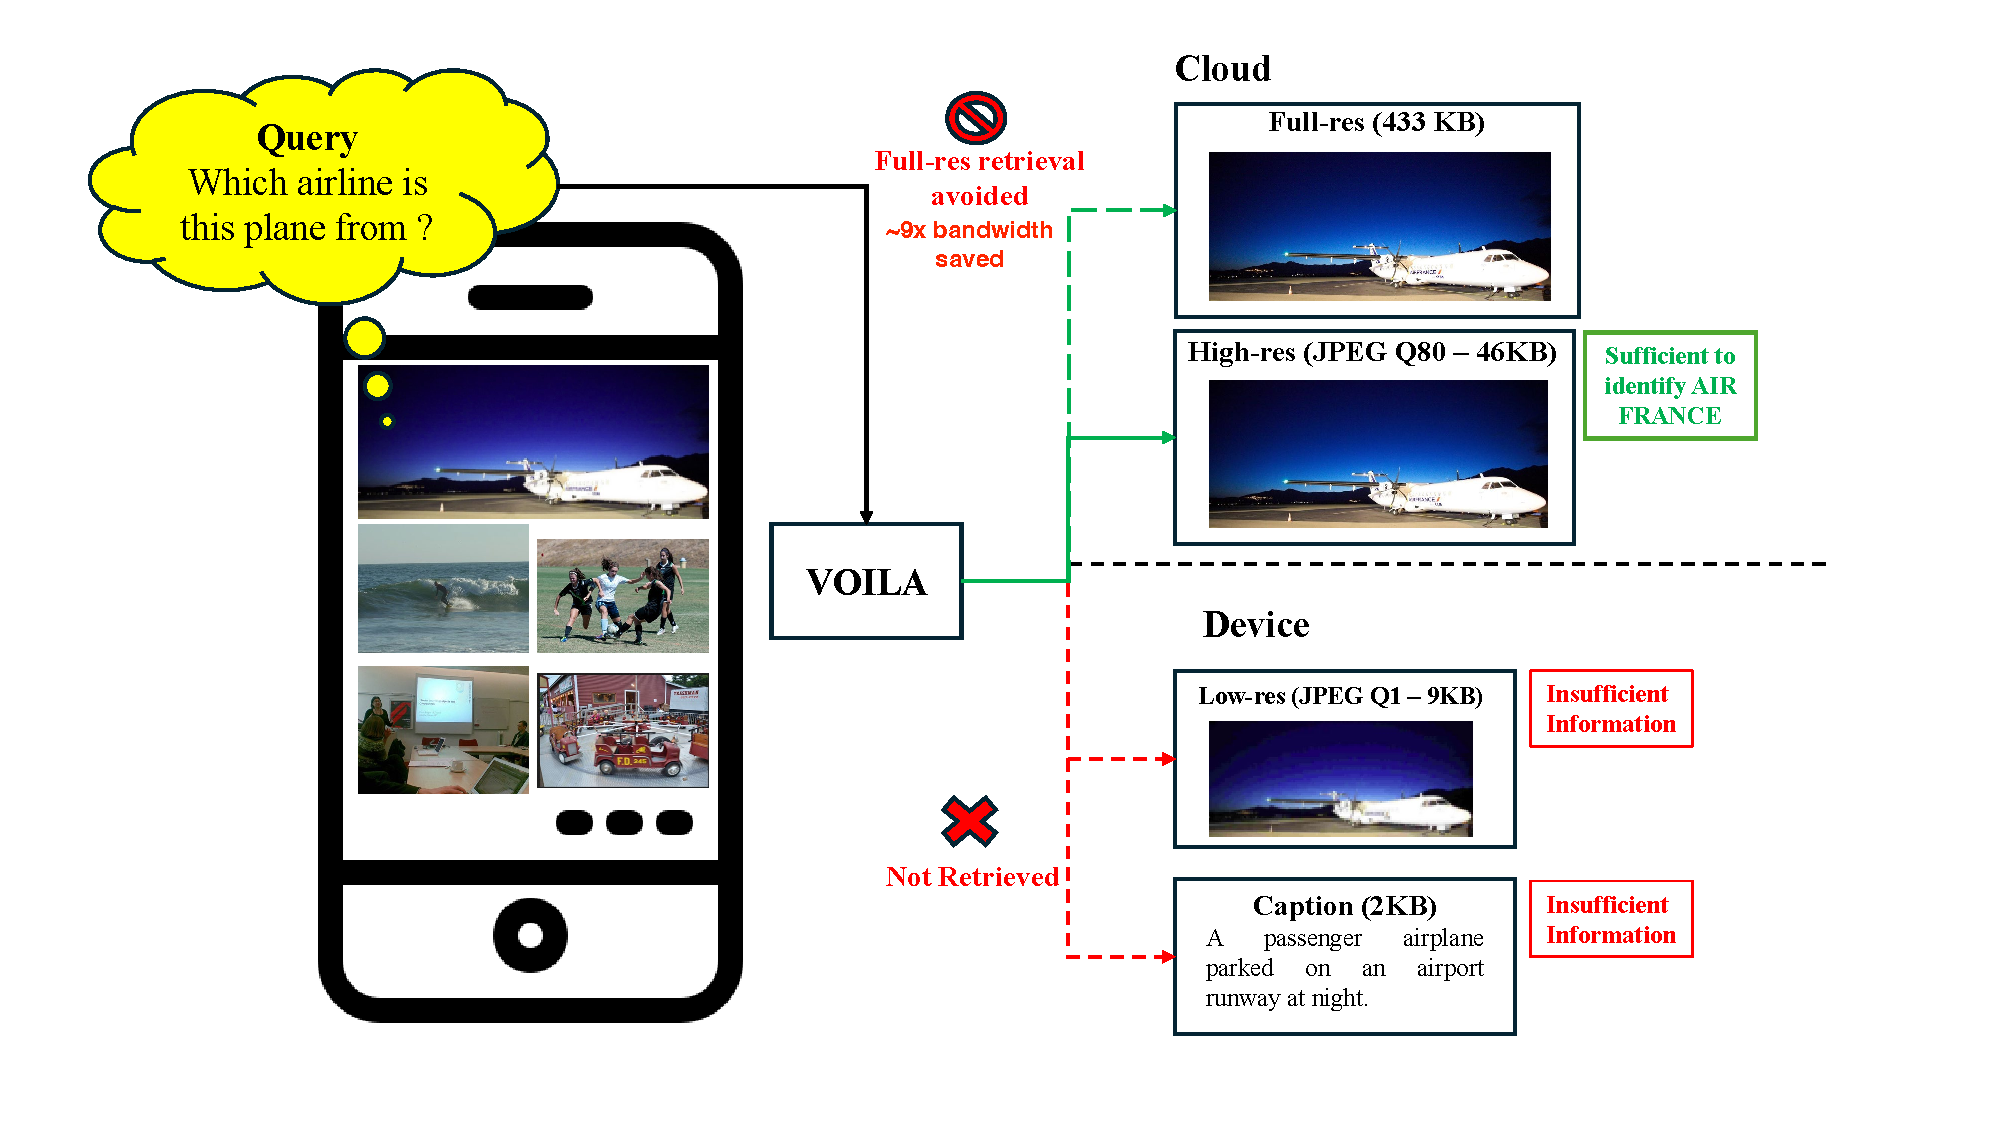
\includegraphics[width=0.9\linewidth]{figures/voila_overview.pdf}
    \caption{VOILA predicts the minimum visual fidelity required to answer a query \emph{before} any image is retrieved. For ``Which airline is this plane from?''---an OCR-dependent question---VOILA selects a mid-fidelity JPEG (46 KB) that preserves the airline logo, avoiding full-resolution retrieval (433 KB) and achieving a 9$\times$ bandwidth reduction.}
    \label{fig:obs1}
\end{figure}

\begin{figure*}[h]
    \centering
    \subfloat[Each curve traces accuracy vs.\ fidelity for one question type; stars mark the first fidelity achieving 95\% of full-resolution accuracy. Counting and OCR tasks require full resolution; yes/no and color saturate at JPEG Q10 (cost 53.2).\label{fig:obs1_dist}]{%
        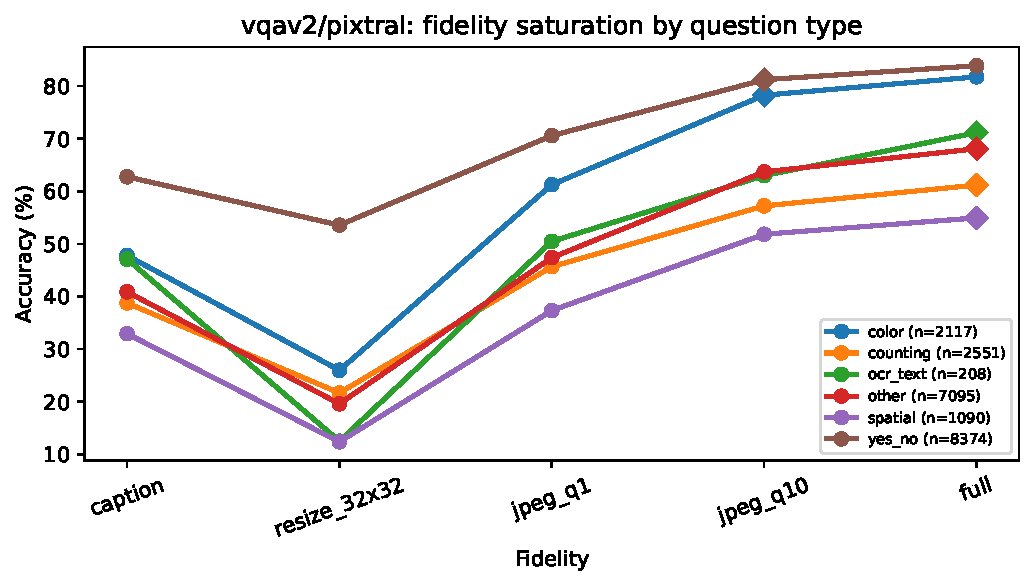
\includegraphics[width=0.32\linewidth]{plots/fidelity_saturation_vqav2_pixtral.pdf}
    }
    \hfill
    \subfloat[VLM output log-probabilities are unreliable indicators of context sufficiency: incorrect low-fidelity answers receive confidence scores comparable to correct ones.\label{fig:obs2_confidence}]{%
        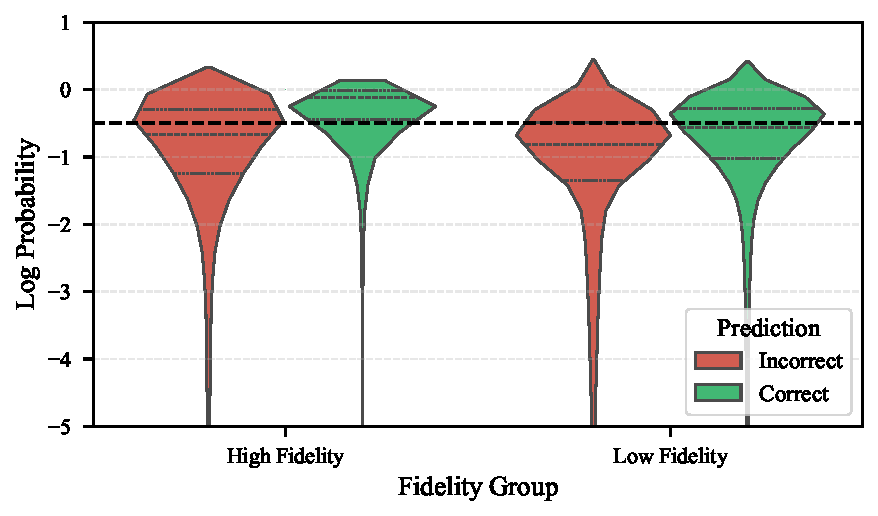
\includegraphics[width=0.32\linewidth]{plots/logprob_collapsed_fidelity_comparison.pdf}
    }
    \hfill
    \subfloat[Model scaling does not compensate for insufficient fidelity: accuracy saturates or degrades at low fidelity regardless of model size.\label{fig:model_scaling_fidelity}]{%
        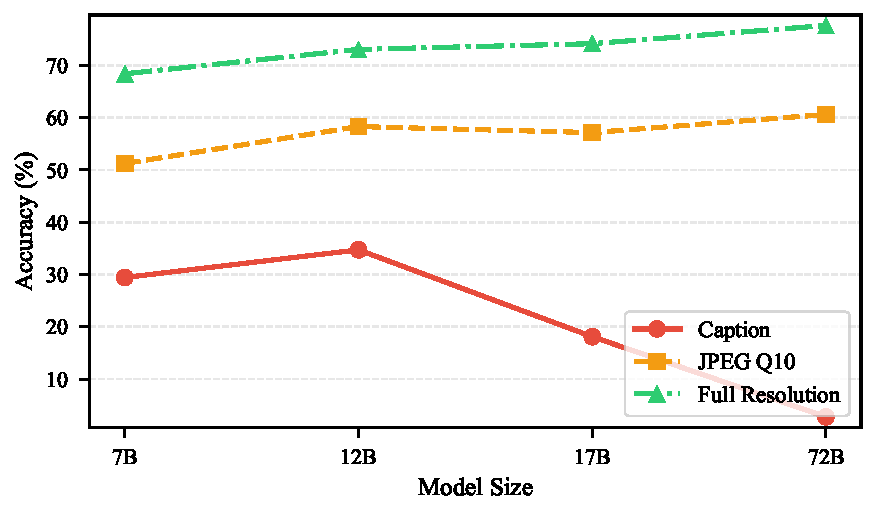
\includegraphics[width=0.32\linewidth]{plots/model_scaling_fidelity_accuracy.pdf}
    }
    \caption{Three empirical observations on VQA-v2 with Pixtral-12B that motivate VOILA's design: (a) question type reliably predicts fidelity requirements; (b) post-hoc confidence signals are unreliable for escalation decisions; (c) model scaling cannot substitute for adequate visual information.}\label{fig:observations_combined}
\end{figure*}

We formalize this as \emph{pre-retrieval fidelity selection} and introduce \textbf{VOILA} (\underline{V}alue-\underline{O}f-\underline{I}nformation guided \underline{L}atency-\underline{A}ware fidelity selection): a gradient-boosted classifier over question features estimates per-fidelity correctness probabilities, isotonic calibration converts raw scores into reliable probabilities, and a greedy value-of-information rule selects the minimum-cost sufficient fidelity---all before any retrieval cost is incurred, with regret bounded by calibration error (Appendix~\ref{sec:theory}).

This paper makes the following contributions:

\begin{itemize}[nosep]
    \item \textbf{Problem formulation:} Pre-retrieval fidelity selection for multimodal RAG---distinct from post-retrieval cascades and from concurrent methods that still require image access---with a near-Bayes-optimal greedy policy under calibrated estimation (\S\ref{sec:method}, Appendix~\ref{sec:theory}).

    \item \textbf{Empirical finding:} Question linguistic structure (\emph{how many}, \emph{what color} vs.\ \emph{is there}, \emph{does it show}) is a strong, sufficient signal for fidelity routing without image access (\S\ref{sec:background}).
    \fablenote{``sufficient'' overclaims: your own error analysis shows 23--25\% under-escalation where linguistic structure does NOT determine the right fidelity. Write ``strong and practically useful'' and explicitly acknowledge the residual visual-context dependence --- pre-empting the obvious counterexample (``How many people?'' over a crowd vs.\ two people) makes the claim more credible, not less.}

    \item \textbf{VOILA framework:} A model-agnostic GBR\,+\,isotonic-calibration system running in 0.45\,ms per query on CPU, with no VLM involvement at decision time (\S\ref{sec:method}).

    \item \textbf{Evaluation} across six VLMs (7B--235B) and five datasets: 50--65\% cost reduction, matching or exceeding full-resolution on OCR-heavy and specialized benchmarks, within 10 accuracy points (average) on general VQA.
\end{itemize}

\fablenote{Contribution list polish for AAAI: (1) the theory (near-Bayes-optimality, regret bounded by calibration error) is currently buried inside the problem-formulation bullet --- AAAI values theory; promote it to its own contribution bullet and state the regret bound informally in one line. (2) The intro never states the headline \emph{against baselines}, only against full-resolution; add ``outperforms log-prob cascades and an LLM router on the accuracy--cost Pareto frontier'' so the contribution is positioned against prior methods, not just a fixed policy. (3) The VOILA acronym is expanded here as ``Latency-Aware'' but the title says ``Fidelity Selection''; make the expansion consistent.}

% -----------------------------------------------------------------------
% OLD INTRODUCTION TEXT (kept for reference)
% -----------------------------------------------------------------------
\begin{comment}
Modern multimodal vision-language systems achieve remarkable accuracy on visual reasoning tasks by scaling models and training data~\cite{alayrac2022flamingo, li2023blip2, liu2024visual}, incurring substantially higher storage, bandwidth, and computational overheads. Recent work has addressed this by focusing on \emph{model selection} and \emph{adaptive routing} -- dynamically choosing between lightweight and heavyweight models based on query characteristics~\cite{chen2023frugalgpt, ding2024hybrid, wang2024routellm}. While reducing \emph{inference costs}, these approaches implicitly assume that input context is fixed and freely available.

In practice, this assumption rarely holds. Multimodal inputs often reside across heterogeneous storage tiers with varying retrieval latencies and costs. Mobile services like Google Photos and iCloud Photos store images at multiple resolutions: on-device caches contain compressed thumbnails and captions, while full-resolution originals reside in cloud storage~\cite{lonn2019smartphonepictureorganizationhierarchical, toderici2016variablerateimagecompression}. Similarly, enterprise systems use hot storage (e.g., AWS S3 Standard) for frequently accessed data and cold storage (e.g., AWS Glacier) for archival content, with retrieval latencies measured in minutes to hours~\cite{aws_s3_storage_classes}. Critically, these retrieval costs are incurred \emph{before} any model processes the input, making post-hoc model routing insufficient for end-to-end efficiency.

We argue that \textbf{context selection at the pre-retrieval stage is a distinct and fundamental learning problem}, orthogonal to model routing. Before asking \emph{which model should answer this query?}, we ask: \emph{Which representation of the available context should be retrieved at all}? Figure~\ref{fig:obs1} shows that for ``Which airline is this plane from?'', a VLM cannot answer from a caption (2 KB) but identifies ``Air France'' from a compressed JPEG (46 KB), avoiding full-resolution retrieval (433 KB)—a 9$\times$ reduction. \textbf{Different queries need different fidelities}, predictable before retrieval.
\end{comment}


% -----------------------------------------------------------------------
% REWRITTEN: Section renamed for EMNLP; observations sharpened with
% linguistic framing.
% -----------------------------------------------------------------------

\section{Question Semantics Predict Visual Information Requirements}\label{sec:background}\label{sec:emp_insights}

\fablenote{For AAAI, consider retitling to ``Why Pre-Retrieval Fidelity Selection Is Both Necessary and Tractable'' --- the current title is NLP-flavored; the proposed one states the two claims the section actually proves and matches a broad-AI audience. Also: all three observations are derived from VQA-v2 + Pixtral-12B with a one-line ``patterns hold across all six models'' assurance. A+ standard is to show the replication, not assert it --- add a small table or appendix pointer with the key statistic (e.g., log-prob AUC, saturation fidelity per question type) for at least 2--3 models.}

We present three empirical observations that collectively establish (i) the practical importance of the pre-retrieval fidelity selection problem and (ii) the tractability of solving it from question text alone.
All observations are based on VQA-v2 with Pixtral-12B across input fidelities ranging from text-only captions to full-resolution images (Figure~\ref{fig:observations_combined}), with qualitatively identical patterns across all six evaluated models.

\textbf{Observation 1: Fidelity Requirements Are Linguistically Predictable.}
Figure~\ref{fig:obs1_dist} shows that query type strongly predicts minimum required fidelity.
Questions containing \emph{how many}, \emph{what color}, or \emph{read/what does it say} signal subtasks requiring fine-grained evidence (object counting, hue discrimination, OCR) that low-fidelity representations destroy; questions containing \emph{is there}, \emph{does the image show}, or \emph{what type} involve coarse semantic judgments resolvable from captions or thumbnails.
On VQA-v2, yes/no and color questions plateau at JPEG Q10 (cost 53.2), while counting, OCR, and spatial queries require full resolution (cost 100).
No single fidelity dominates, establishing that fidelity selection is both necessary and tractable from question text alone~\cite{kafle2017analysis,agrawal2018dont}.
Under-escalation errors (23--25\% of queries, \S\ref{sec:results}) reflect cases where the correct fidelity depends on visual context rather than linguistic structure---the main reducible component of the Oracle--\textsc{VOILA} gap.

\textbf{Observation 2: Post-Retrieval Confidence Is an Unreliable Escalation Signal.}
FrugalGPT-style cascades~\cite{chen2023frugalgpt} retrieve low-cost context first and escalate when VLM log-probability falls below a threshold.
This fails in the fidelity domain: as Figure~\ref{fig:obs2_confidence} shows, incorrect low-fidelity answers receive log-probabilities comparable to---or exceeding---correct ones (43\% of incorrect caption-fidelity answers on VQA-v2 exceed the median log-probability of correct caption-fidelity answers).
For Qwen2-VL-72B, the log-probability AUC for caption-to-full escalation is 0.338---\emph{below random} (ROC curves in Appendix~\ref{sec:ablations})---confirming VLM confidence is an actively misleading escalation signal at low fidelity.
\fablenote{Observation 2 is the paper's strongest novel finding and deserves one sentence of \emph{mechanism}: WHY is confidence anti-correlated at low fidelity? (Plausible: with no visual grounding the VLM falls back on language priors, and prior-driven answers are fluent and hence high-probability.) A causal sentence here turns a curious statistic into an insight reviewers will cite. Also report AUC for all six models, not just the worst one --- cherry-picking the 0.338 invites suspicion that other models are near 0.5.}

\textbf{Observation 3: Model Scaling Does Not Substitute for Sufficient Visual Information.}
Figure~\ref{fig:model_scaling_fidelity} shows that fixing input fidelity at a low level caps accuracy regardless of model size: caption-only accuracy saturates or \emph{degrades} at larger scale (likely due to hallucination when visual grounding is absent), while full-resolution accuracy improves consistently with scale.
Model scaling and information acquisition are therefore \emph{complementary rather than substitutable} optimization axes---the key motivation for pre-retrieval fidelity selection.

These observations establish that fidelity requirements are (1) linguistically predictable pre-retrieval, (2) not estimable from post-hoc confidence, and (3) not compensated by model scaling---motivating \textsc{VOILA}'s design.

\begin{comment}
% OLD OBSERVATION TEXT (kept for reference)
\textbf{Observation 1 (old).}
Figure~\ref{fig:obs1} in the previous section showed that different questions over the same image require different minimum input fidelities. Figure~\ref{fig:obs1_dist} quantifies this at scale: low-fidelity representations (captions, thumbnails) succeed on semantically coarse queries (yes/no, some object identification) but fail disproportionately on counting, color, spatial, and OCR tasks requiring fine-grained visual evidence.
In contrast, high-fidelity inputs substantially improve accuracy on these visually demanding categories while offering limited gains on queries already solvable at low fidelity. No single fidelity dominates across query types, motivating query-adaptive fidelity selection.
\end{comment}


\section{VOILA: Query-Conditioned Fidelity Selection}\label{sec:method}

\subsection{Problem Formulation} Let $(q, x)$ denote a visual question $q$ paired with an image $x$.
We assume access to a discrete, ordered set of input fidelities $\mathcal{F} = \{f_1, f_2, \dots, f_K\}$,
sorted by increasing acquisition cost, where each fidelity $f \in \mathcal{F}$ incurs a cost $c(f) > 0$ capturing retrieval latency, bandwidth, and compute overhead.
Lower fidelities correspond to inexpensive representations (e.g., captions or thumbnails), while higher fidelities provide richer visual information (e.g., full-resolution images).

%However, executing the VLM at multiple fidelities to empirically determine which works is prohibitively expensive at inference time.

For fidelity $f$, if the vision--language model (VLM) produces an answer $\hat{a}_f$, our objective is to select the fidelity that maximizes expected utility:
\[
f^\star
=
\arg\max_{f \in \mathcal{F}}
\underbrace{\Pr(\hat{a}_f \text{ is correct} \mid q)}_{\text{expected accuracy}} - \underbrace{\lambda c(f)}_{\text{acquisition cost}},
\]
where \textbf{the probability of correctness must be estimated \emph{without} retrieving fidelity $f$ or running the VLM at that fidelity}, and $\lambda$ controls the accuracy-cost trade-off. VOILA accomplishes this through question-conditioned learned estimators.
\fablenote{AAAI framing opportunity: this objective is a one-step value-of-information decision; say so here and cite the decision-theoretic lineage (Howard 1966, VOI; cost-sensitive feature acquisition). One sentence connecting $f^\star$ to the Bayes-optimal acquisition policy (currently hidden in Appendix theory) lifts the section from ``engineering pipeline'' to ``principled method'' --- the single highest-leverage writing change for an AAAI audience.}

%This seemingly impossible requirement---predicting VLM success without running the VLM---is what VOILA 



\subsection{Design Overview: A Three-Stage Pipeline}

VOILA adopts a three-stage pipeline: (1)~\textbf{question-conditioned success scoring} (\S\ref{sec:success_scoring}) predicts, from question features alone, how likely each fidelity is to yield a correct answer; (2)~\textbf{fidelity-specific calibration} (\S\ref{sec:voila_calibration}) converts raw scores into reliable probabilities; and (3)~\textbf{VOI selection} (\S\ref{sec:voi}) picks the minimum-cost fidelity whose expected accuracy gain justifies retrieval cost.


\subsection{Question-Conditioned Success Scoring}\label{sec:success_scoring}

%\paragraph{Motivation.} 
Fig.~\ref{fig:observations_combined} illustrates that question features contain predictive signal about cross-fidelity performance \emph{before} any visual information is retrieved. To exploit this signal, we construct training data by executing the VLM at each fidelity $f$ on labeled examples and recording whether the produced answer is correct. Let $y_f \in \{0,1\}$ denote the correctness label for fidelity $f$. We extract a question feature representation $\phi(q)$ consisting of:
\begin{itemize}[nosep]
    \item TF--IDF features of the question text (top-5{,}000 unigram vocabulary computed over the training split),
    \item lexical statistics: question length, presence of numeric tokens, superlatives, and negations,
    \item question-type indicators: five binary flags derived by rule-based matching on question-initial words and syntactic patterns (counting: \emph{how many}; yes/no: \emph{is/are/does/do}; color: \emph{what color}; spatial: \emph{where}; OCR/text: \emph{read/spell/say/written}).
\end{itemize}

We deliberately use lightweight, interpretable features rather than large pretrained encoders (e.g., BERT or sentence transformers) for two reasons.
First, it demonstrates that the task is solvable from surface-level linguistic structure alone---the central empirical claim of this paper.
Second, TF-IDF feature extraction requires no GPU and completes in under 1\,ms, making \textsc{VOILA} deployable on edge devices without a pretrained language model dependency.
The combined feature vector has 5{,}017 dimensions (5{,}000 TF-IDF + 12 lexical + 5 question-type).
Figure~\ref{fig:routing_words} (Appendix~\ref{sec:ablations}) visualizes the top-ranked TF-IDF features: words predictive of caption sufficiency (\emph{is}, \emph{there}) differ systematically from those predicting full-resolution need (\emph{color}, \emph{many}, \emph{sport}).

\fablenote{This paragraph (feature ablation + OOD transfer + vocabulary-size discussion) is results material living in the method section, and it partially duplicates \S\ref{sec:results}. Cut it to one sentence with a forward reference, and reclaim the ~12 lines for what the method section is missing: a worked end-to-end example (one real question, its features, the five calibrated probabilities, the VOI computation, the selected fidelity). A concrete trace is the fastest way for a reviewer to verify they understand the method.}
Feature ablation experiments (Table~\ref{tab:feature_ablation}, \S\ref{sec:results}) confirm that the full 5{,}017-dimensional combination achieves the best in-distribution accuracy--cost Pareto position. Crucially, question-type flags alone are competitive under cross-dataset transfer: trained on VQA-v2 and evaluated on GQA, TextVQA, and FloodNet without retraining, they retain 79--92\% of in-domain routing accuracy, whereas TF-IDF vocabulary degrades more sharply under domain shift because it encodes corpus-specific word statistics rather than language-universal syntactic roles (on FloodNet, question-type-only routing achieves 53.1\% OOD accuracy vs.\ 42.7\% for TF-IDF-only). The TF-IDF vocabulary size of 5{,}000 is a conservative high-capacity default; ablation experiments show no monotonic gain from increasing vocabulary size (performance is comparable at 1{,}000--2{,}000 tokens), so 5{,}000 is retained as a robust upper bound.

Using these features, we train a fidelity-specific regressor
\[
r_f(q) = g_f(\phi(q))
\]
to produce a raw score that correlates with the likelihood that the VLM will answer correctly at fidelity $f$. \textbf{Crucially, $g_f$ is a learned estimator of VLM behavior, not the VLM itself.} The regressor learns statistical patterns between question characteristics and cross-fidelity success rates during offline training. At inference time, \textbf{computing $r_f(q)$ requires only a forward pass through a lightweight tree ensemble---no visual retrieval, no VLM execution, no multimodal processing}. This is orders of magnitude faster and cheaper than actually running the VLM at each fidelity.



%\paragraph{Why Gradient Boosting Regressors (GBR)?}
We use a Gradient Boosting Regressor~\cite{prettenhofer2014gradient} for $g_f$: it handles high-dimensional sparse TF-IDF inputs naturally and captures non-linear question--fidelity interactions (e.g., ``counting + small objects'' $\Rightarrow$ high fidelity) without manual feature engineering. Predictor ablations (\S\ref{sec:results}) confirm calibration quality matters more than model choice; GBR, logistic regression, ridge, and MLP all perform similarly under isotonic calibration.





\subsection{Fidelity-Specific Probability Calibration}
\label{sec:voila_calibration}

%\paragraph{Motivation.}
The regressor output $r_f(q)$ is \emph{not} a calibrated probability; rather, it is a \emph{question-conditioned success score} that orders queries by their relative likelihood of being answered correctly by the vision--language model at fidelity $f$.
%Uncalibrated scores exhibit severe overlap between correct and incorrect predictions, making them unsuitable for reasoning about expected utility. Without calibration, high raw scores do not reliably indicate high success probability, leading to systematic over- or under-escalation.
Because $r_f(q)$ is not probabilistic, we apply fidelity-specific post-hoc calibration using isotonic regression~\cite{guo2017calibrationmodernneuralnetworks}.
For each fidelity $f$, we fit an isotonic regression model
\[
\psi_f: r_f(q) \mapsto \hat{p}_f(q),
\]
on a held-out 20\% split of the training data (disjoint from both GBR training and evaluation test sets), where $\hat{p}_f(q) \in [0,1]$ estimates the probability that the vision--language model would answer question $q$ correctly if executed at fidelity $f$.
All datasets are split 75\%/25\% into training and evaluation sets; within the training portion, 80\% is used for GBR training and 20\% for isotonic calibration (i.e., 60\% / 15\% / 25\% of the full dataset).
Isotonic regression is non-parametric and fits in $O(n \log n)$ time; at the dataset sizes we use (3{,}000--12{,}000 examples per fidelity), it does not require cross-validation and is not prone to overfitting. By fitting a non-decreasing mapping from raw scores to empirical success frequencies on held-out data, isotonic regression enforces monotonicity by construction and corrects systematic over- and under-confidence in the raw scores.
This calibration step uses only $(r_f(q), y_f)$ pairs, where $y_f \in \{0,1\}$ denotes historical correctness at fidelity $f$. %\paragraph{Why Isotonic Regression?}
Isotonic regression is non-parametric (no assumptions on miscalibration shape), preserves the score rank ordering learned by the regressor, and has well-understood convergence guarantees~\cite{guo2017calibrationmodernneuralnetworks} (formal bounds in Appendix~\ref{sec:calibration}).
\textbf{Cross-fidelity monotonicity.}
The per-fidelity calibrators above enforce monotonicity \emph{within} each fidelity's score-to-probability mapping, but do not guarantee that $\hat{p}_{f_1}(q) \leq \hat{p}_{f_2}(q) \leq \cdots \leq \hat{p}_{f_K}(q)$ holds \emph{across} fidelity levels for a given query.
In practice, average accuracy need not be monotone in fidelity (e.g., on TextVQA, VLM-generated captions often score higher than low-quality thumbnails because they already encode scene text).
To guarantee that the greedy escalation policy of Algorithm~\ref{alg:voila} finds the global utility optimum, we apply a lightweight secondary isotonic regression pass \emph{across} fidelity levels on the per-query calibrated scores at inference time, enforcing the ordering $\hat{p}_{f_1}(q) \leq \dots \leq \hat{p}_{f_K}(q)$.
This step adds negligible overhead ($<$0.01\,ms) and removes non-unimodal utility cases that would otherwise cause the greedy break to terminate prematurely.

\textbf{The key effect of isotonic calibration is probability reliability.}
Figure~\ref{fig:cali:scatter} shows reliability diagrams for VQA-v2/Pixtral-12B: isotonic calibration closely tracks the perfect-calibration diagonal, while raw GBR scores and VLM log-probabilities deviate substantially (ECE: 0.025\,$\to$\,0.012; Brier: 0.205\,$\to$\,0.203).
\fablenote{The Brier improvement (0.205$\to$0.203) is negligible and quoting it weakens the claim --- a careful reviewer will note that calibration barely moved Brier and ask why the paper calls calibration ``the central enabler.'' Either explain (ECE measures calibration, Brier conflates calibration with discrimination, and isotonic regression by design preserves discrimination) or drop the Brier numbers here and let the downstream routing ablation (10--25\% cost reduction) carry the argument.}
When $\hat{p}_f(q)$ reliably estimates the true correctness probability, the VOI gain $\hat{p}_{f’}(q) - \hat{p}_f(q)$ becomes an accurate predictor of the accuracy improvement from escalation.
Additional model--dataset pairs are in Appendix~\ref{sec:ablations} (Figure~\ref{fig:reliability}).

\begin{figure}[tb]
    \centering
    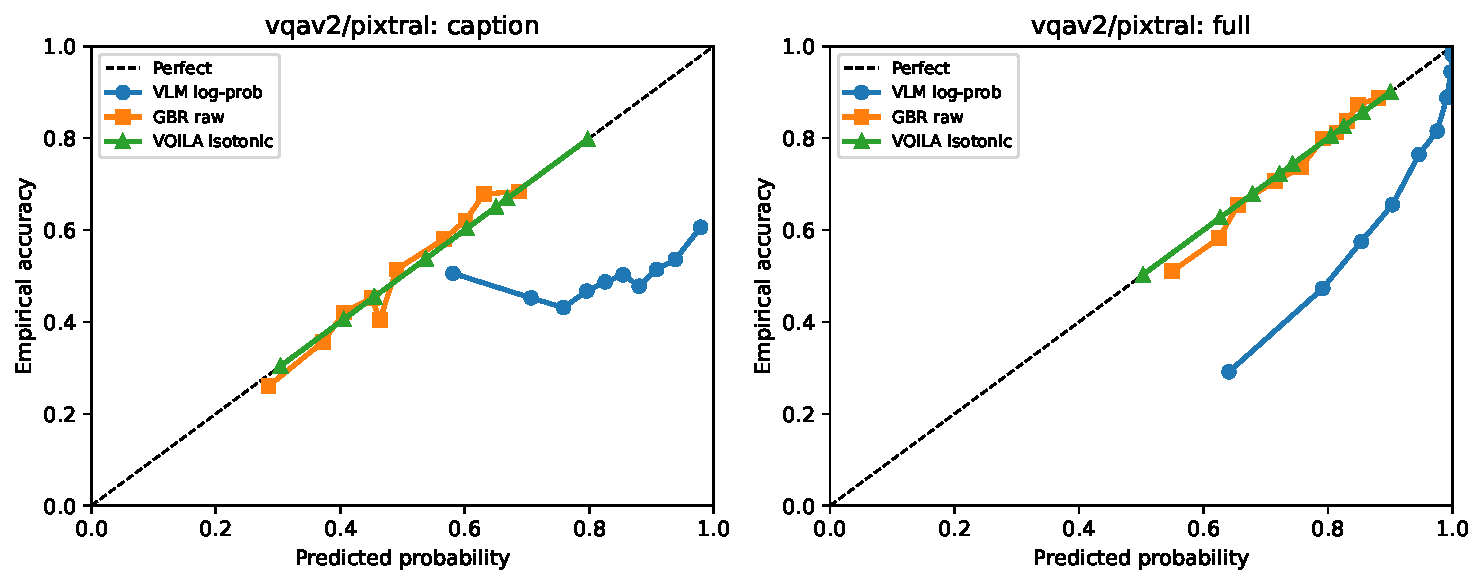
\includegraphics[width=\linewidth]{plots/reliability_vqav2_pixtral.pdf}
    \caption{\textbf{Reliability diagram} (VQA-v2, Pixtral-12B). Isotonic calibration closely tracks the perfect-calibration diagonal (dashed); raw GBR scores and VLM log-probabilities deviate substantially, causing log-prob cascades to under-escalate (Observation~2).}
    \label{fig:cali:scatter}
\end{figure}



\begin{comment}





\subsection{Fidelity-Specific Probability Calibration}\label{sec:calibration}

\begin{figure}[h]
    \centering
    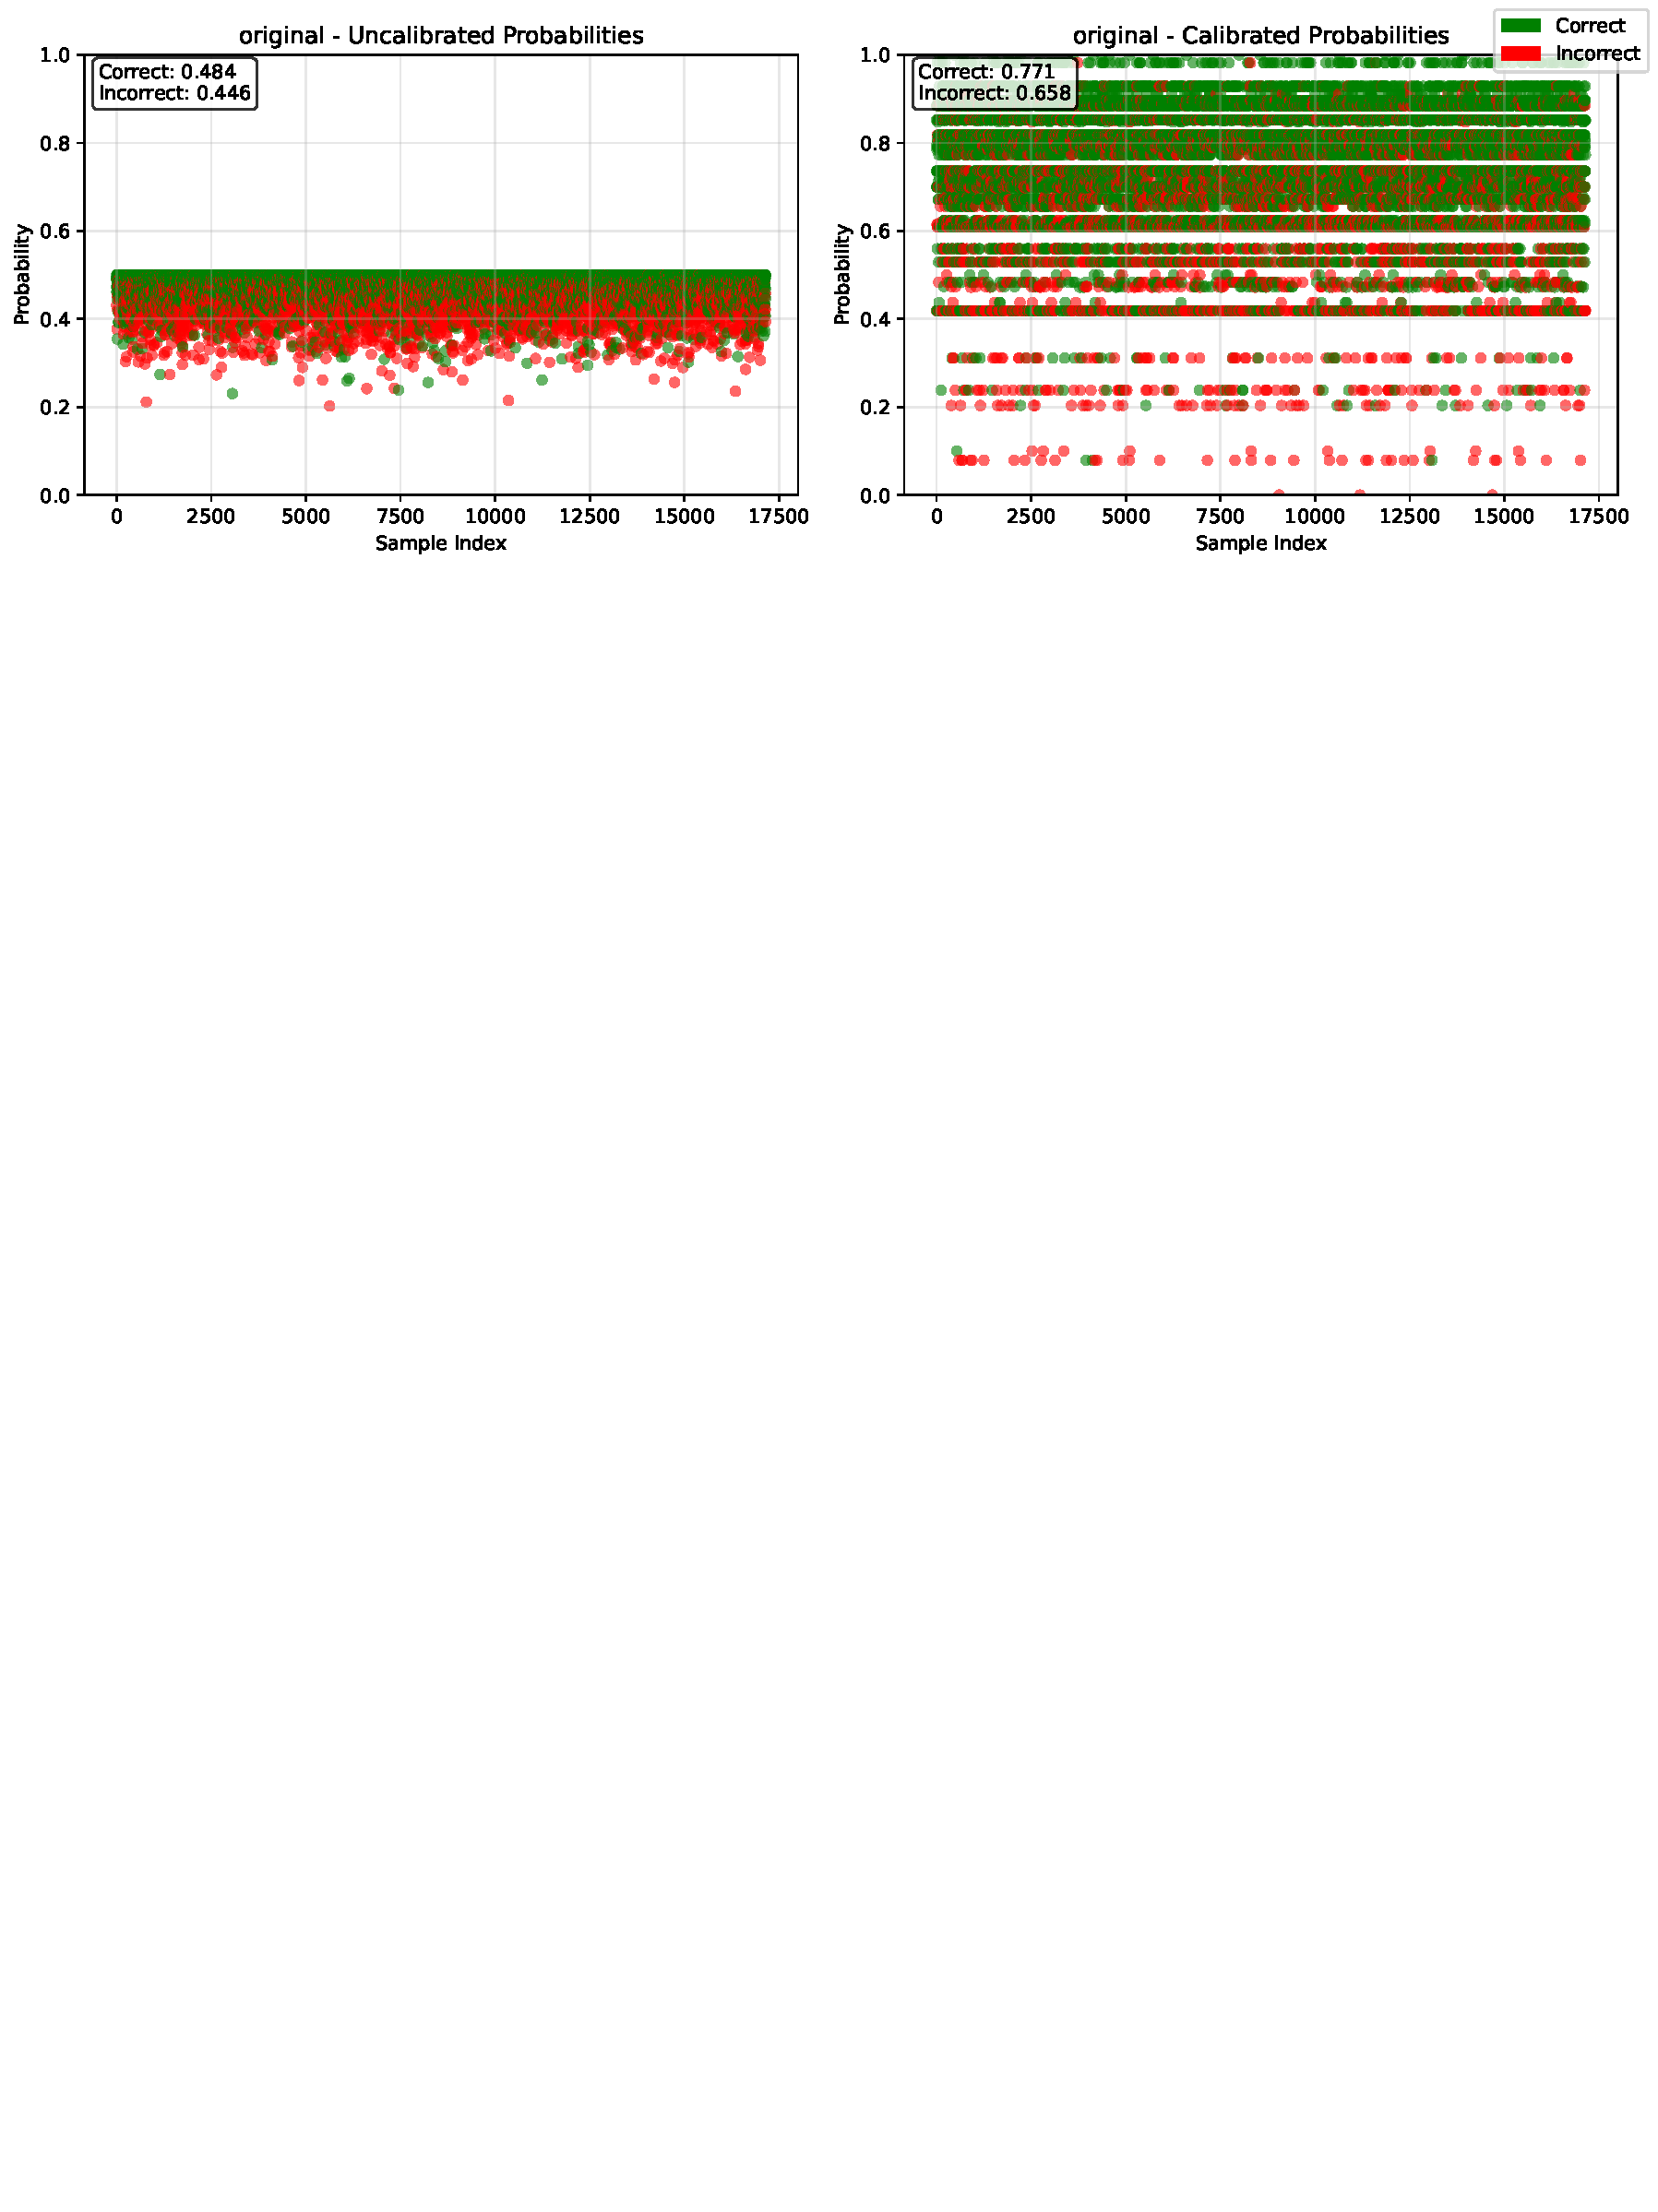
\includegraphics[width=\linewidth]{plots/calibrated_vs_uncalibrated_scatter_1.pdf}
    \caption{Calibrated vs. uncalibrated probabilities}
%Each point shows the predicted correctness probability for a query, colored by outcome.
%Uncalibrated predictors produce overlapping probabilities for correct and incorrect answers, while isotonic calibration yields well-separated, monotonic estimates that enable reliable value-of-information decisions across fidelities.}

    \label{fig:cali:scatter}
\end{figure}

The raw scores $r_f(q)$ produced by the regressor are \emph{not} calibrated probabilities. As demonstrated in Figure~\ref{fig:cali:scatter}, raw uncalibrated scores exhibit severe overlap between correct and incorrect predictions across all fidelities, making them unsuitable for reasoning about expected utility. Without calibration, high raw scores do not reliably indicate high success probability, leading to systematic over- or under-escalation. After isotonic calibration, however, the predicted probabilities become both more dispersed and better aligned with empirical correctness: correct predictions are consistently shifted toward higher probabilities, while incorrect ones are pushed downward, yielding clearer separation across caption, JPEG, and full-resolution inputs.


%\textbf{Observation 4: Calibration Enables Reliable Utility-Aware Decisions}: Figure~\ref{fig:cali:scatter} shows that raw, uncalibrated success probabilities provide little separation between correct and incorrect answers across all fidelities: predicted probabilities are tightly clustered, with substantial overlap between outcomes, making them unsuitable for reasoning about the expected benefit of escalation.  This calibrated behavior is crucial for value-of-information reasoning, as it ensures that predicted gains from acquiring higher-cost fidelities correspond to real accuracy improvements. As a result, VOILA can make stable, interpretable utility-aware decisions—escalating only when the expected benefit justifies the cost—whereas uncalibrated predictors or heuristic thresholds lack a reliable notion of marginal value and lead to inconsistent or unnecessary escalation.


%\paragraph{Motivation.}

%\paragraph{Design Decision: Isotonic Regression.}
To obtain reliable probability estimates, we apply fidelity-specific post-hoc calibration. For each fidelity $f$, we fit an isotonic regression model
\[
\psi_f: r_f(q) \mapsto \hat{p}_f(q),
\]
on a held-out calibration split, where $\hat{p}_f(q) \in [0,1]$ estimates the probability that the VLM would answer correctly at fidelity $f$.
\textbf{The key effect of calibration is separation}: isotonic regression transforms overlapping, uninformative raw scores into well-separated probabilities where correct predictions cluster near 1.0 and incorrect predictions cluster near 0.0 (Figure~\ref{fig:cali:scatter}). This separation enables VOILA to reliably distinguish queries that will succeed at low fidelity from those requiring higher fidelity---\emph{without ever running the VLM}. The calibrator learns this mapping purely from question features $\phi(q)$ and historical correctness labels $y_f$. At inference time, only the calibrated predictor $\hat{p}_f(q)$ is used; no additional calibration or model execution is required.

%\paragraph{Why Isotonic Regression?}
Isotonic regression offers VOILA three critical properties, when compared to other calibration techniques:
\begin{enumerate}[nosep]
    \item \textbf{Monotonicity preservation}: Ensures that higher raw scores always map to higher probabilities, maintaining the rank ordering learned by the regressor.
    \item \textbf{Non-parametric}: Makes no assumptions about the functional form of miscalibration, allowing it to correct arbitrary systematic biases.
    \item \textbf{Proven calibration guarantees}: Isotonic regression is a standard tool in probability calibration with well-understood convergence properties.
\end{enumerate}

%As shown in Figure~\ref{fig:cali:scatter}, isotonic calibration transforms overlapping, uninformative score distributions into well-separated, reliable probabilities that enable stable value-of-information reasoning. 


\end{comment}


\subsection{Value-of-Information--Based Fidelity Selection}
\label{sec:voi}

%\paragraph{Motivation.}
With calibrated success probabilities $\hat{p}_f(q)$ in hand---\textbf{computed from question features alone, without any VLM execution}---we can now reason explicitly about the \emph{marginal value} of acquiring higher-cost fidelities. The key insight is that we should escalate to a more expensive representation only when the expected improvement in accuracy justifies the additional acquisition cost.
%\paragraph{Design Decision: Greedy VOI Escalation.}

Starting from the lowest-cost fidelity $f_1$, VOILA evaluates whether escalating to the next higher fidelity $f_j$ is beneficial by computing the \textbf{Value of Information (VOI)}:
\[
\mathrm{VOI}(f_j \mid f_i)
=
\underbrace{[\hat{p}_{f_j}(q) - \hat{p}_{f_i}(q)]}_{\text{expected accuracy gain}} - \underbrace{\lambda c(f_j)}_{\text{acquisition cost}}.
\]

\textsc{VOILA} incrementally increases fidelity only when $\mathrm{VOI}(f_j \mid f_i) > \tau$, i.e., when the expected improvement in correctness outweighs the additional acquisition cost, where $\tau$ is a decision threshold and $\lambda$ is a cost penalty.
Both $\lambda$ and $\tau$ are tuned by grid search on the validation split of each training dataset; $\tau = 0$ (escalate whenever expected gain exceeds cost) serves as a strong default, and \textsc{VOILA} is robust to moderate changes in $\lambda$ because it depends only on relative cost differences between fidelities (full sensitivity analysis in Appendix~\ref{sec:reproducibility}).
The greedy policy requires only $K$ forward passes through the calibrated predictors (no tree search), is near-optimal under the diminishing-returns assumption (Corollary~1, Appendix~\ref{sec:regret}), and exposes the interpretable cost-tradeoff knobs $\lambda$ and $\tau$.

\begin{algorithm}[tb]
\caption{\textsc{VOILA} Inference Procedure}
\label{alg:voila}
\small
\begin{algorithmic}[1]
\State \textbf{Input:} Query $q$, fidelity set $\mathcal{F}=\{f_1,\ldots,f_K\}$, $\lambda$, $\tau$
\State \textbf{Output:} Selected fidelity $f^*$ and answer $\hat{a}_{f^*}$
\State $f \gets f_1$;\; $\hat{p} \gets \psi_{f_1}(r_{f_1}(q))$ \hfill\Comment{no image, no VLM}
\For{$f' \in \{f_2, \ldots, f_K\}$ in ascending cost order}
    \State $\hat{p}' \gets \psi_{f'}(r_{f'}(q))$
    \If{$(\hat{p}' - \hat{p}) - \lambda c(f') > \tau$}
        \State $f \gets f'$;\; $\hat{p} \gets \hat{p}'$
    \Else\; \textbf{break}
    \EndIf
\EndFor
\State Retrieve image at fidelity $f$; run VLM; \Return $f,\hat{a}_f$
\end{algorithmic}
\end{algorithm}

\textsc{VOILA} requires no modifications to the underlying VLM; it is compatible with any model that produces discrete correctness labels for offline training. The GBR predictor and isotonic calibrator are trained per VLM on 3,000--12,000 labeled examples per fidelity (minutes on standard hardware), then used at inference time to select the optimal fidelity from question text alone before any visual data is accessed.


%In this section, we describe the design and core algorithms of \textbf{VOILA} (\underline{V}alue-\underline{O}f-\underline{I}nformation guided \underline{L}atency-\underline{A}ware fidelity selection).



%, a query-adaptive framework for selecting the minimum-cost input fidelity required to answer a multimodal query accurately, using \emph{only} features of the question text—\emph{before} retrieving any visual input or executing a vision--language model (VLM).
%While VLMs expose token-level confidence scores after inference, these signals are fundamentally unsuitable for fidelity selection.
%As shown in Figures~\ref{fig:observations_combined} and~\ref{fig:cali:scatter}, VLM confidence exhibits substantial overlap between correct and incorrect predictions when visual information is insufficient, frequently producing confident but incorrect answers at low fidelity.
%Crucially, such confidence scores are available only \emph{after} visual retrieval and model execution, rendering them unusable for pre-retrieval decision-making.



%The key design principle underlying VOILA is simple: \emph{different queries have different minimum information requirements, and these requirements are predictable from the question alone---without ever executing the VLM or retrieving visual content at inference time}.

%\subsection{The Core Challenge: Pre-Retrieval Decision-Making}


%Consider the motivating example from Figure~1: given the query ``Which airline is this plane from?'', we must decide whether to retrieve a caption (2KB), a low-resolution thumbnail (9KB), a compressed image (46KB), or the full-resolution original (433KB) \emph{before} incurring any retrieval or processing costs. This decision must be made using only the question text, as accessing visual content to ``check'' which fidelity works would defeat the purpose of adaptive selection.

%This \textbf{pre-retrieval constraint} distinguishes our problem from existing model routing approaches, which assume all context is freely available and optimize only \emph{which model} to apply. In contrast, VOILA optimizes \emph{which representation of the context to acquire} before any expensive operations occur. \textbf{Critically, VOILA never executes the VLM to determine fidelity selection at inference time}---all predictions are made from question features alone, using lightweight learned estimators trained offline.


\section{Evaluation}\label{sec:experiments}

Our evaluation aims to address three questions: (i) does \textsc{VOILA} consistently improve accuracy-cost trade-offs versus fixed-fidelity baselines? (ii) do gains persist across model scales and datasets? and (iii) which components are performance-critical?
\fablenote{Question (i) sets the bar too low --- fixed-fidelity is the weakest comparison class. Rewrite as ``versus fixed-fidelity policies and adaptive routing baselines (cascades, LLM/BERT routers)''; you already beat those baselines, so claim the harder fight up front. Also add a missing experimental detail AAAI reviewers always check: how many evaluation queries per dataset, how many runs/seeds, and whether differences are statistically significant (bootstrap CIs over queries cost nothing to add and immunize every comparison in \S\ref{sec:results}).}

\textbf{Models.} We evaluate six VLMs: Pixtral-12B~\cite{pixtral2024}, LLaMA-4-Maverick (17B$\times$12E)~\cite{abdullah2025evolutionmetasllamamodels}, LLaVA-1.5-7B~\cite{zhou2024tinyllava}, Qwen2-VL-72B~\cite{Qwen2VL}, Qwen2.5-VL-7B~\cite{Qwen2VL}, and Qwen3-VL-235B~\cite{bai2023qwen}, spanning 7B--235B parameters across architectures from 2023--2025. All models are used zero-shot.

\textbf{Datasets.}
\textbf{VQA-v2}~\cite{goyal2017vqav2} and \textbf{GQA}~\cite{hudson2019gqa} are standard in-domain VQA benchmarks.
\textbf{TextVQA}~\cite{singh2019textvqa} emphasizes OCR-dependent reasoning.
\textbf{FloodNet}~\cite{rahnemoonfar2021floodnet} is a bandwidth-constrained cyber-physical setting (aerial disaster imagery).
\textbf{LoCoMo}~\cite{wang2024locomo}: we generate VQA-style QA pairs from conversational memory items using GPT-4o (details in Appendix~\ref{sec:datasets}).

\textbf{Input Fidelities.}
$\mathcal{F}=\{\texttt{caption},\ \texttt{resize}_{32\times32},\ \texttt{jpeg\_q1},\ \texttt{jpeg\_q10},\ \texttt{full}\}$, ordered by acquisition cost. Captions are generated offline by the target VLM from full-resolution images; caption retrieval cost (7.6) reflects serving a pre-computed string from cache, not one-time generation. Full-resolution cost is normalized to 100 (details in Appendix~\ref{sec:cost_model}).

\paragraph{Cost Model.}
Each fidelity incurs acquisition cost $c(f) = \alpha B(f) + \beta L(f) + \gamma S(f)$, where $B(f)$, $L(f)$, $S(f)$ are empirically measured bandwidth, retrieval latency, and storage-access ratios. Costs reflect input acquisition overhead only; \textsc{VOILA} depends only on relative cost differences.

\textbf{Baselines.}
We compare \textsc{VOILA} against:
\begin{itemize}[nosep]
    \item \textbf{Fixed-fidelity} ($f \in \mathcal{F}$): always retrieve at a single level. Establishes the non-adaptive Pareto frontier.
    \item \textbf{Log-prob Cascade}~\cite{chen2023frugalgpt}: execute VLM at lowest fidelity; escalate if log-probability falls below threshold $\theta$ (tuned per model on VQA-v2 validation). Incurs retrieval and inference costs at every intermediate fidelity.
    \item \textbf{GPT-4o Router} (zero-shot): GPT-4o classifies each question's visual need as low/medium/high (mapped to caption / JPEG Q10 / full). Labels collected once per dataset, shared across all models.
    \item \textbf{BERT Router}: supervised SentenceTransformer (all-MiniLM-L6-v2) predicting the cheapest correct fidelity label directly --- no VOI objective.
    \item \textbf{Oracle}: cheapest fidelity that actually produces a correct answer (hindsight upper bound).
    \item \textbf{\textsc{VOILA}-CDF}: \textsc{VOILA} with VOI replaced by a CDF threshold rule. Ablates cost-aware routing while holding predictor and calibration fixed.
\end{itemize}

\textbf{Evaluation Metrics.}
We report task accuracy (\%) and normalized average retrieval cost per query (full-resolution = 100). For interpretability, we also report the fraction of queries routed to each fidelity level and the accuracy--cost Pareto frontier.
For calibration quality we additionally report Brier score and Expected Calibration Error (ECE) in the ablation studies (\S\ref{sec:results}).
\fablenote{Two-number (Acc, Cost) comparisons make it impossible to rank methods when neither dominates --- exactly the situation in Table~\ref{tab:master_comparison} where the GPT-4o Router has higher accuracy but higher cost than \textsc{VOILA} on VQA-v2. Add a single scalar metric that resolves this: either (a) area under the accuracy--cost curve as $\lambda$ sweeps, or (b) accuracy at matched cost / cost at matched accuracy. Without one, a reviewer can legitimately read Table~1 as ``the LLM router is more accurate.''}


\section{Results and Discussions}
\label{sec:results}

\fablenote{Retitle to ``Results and Discussion'' (singular --- ``Discussions'' is non-standard). Structural suggestion for A+ readability: open the section with a 3-sentence summary paragraph stating the three headline findings before any table, so a skimming reviewer gets the verdict in 10 seconds. The single most valuable addition to this section is the commented-out Pareto-frontier figure above --- restore it (or a 2$\times$2 subset): a frontier plot where \textsc{VOILA}'s $\lambda$-sweep curve dominates every baseline point is the one figure that defuses the ``10 points below full resolution'' objection, because it shows VOILA at EVERY operating point, not one.}

% \begin{figure*}[htb]
%     \centering
%     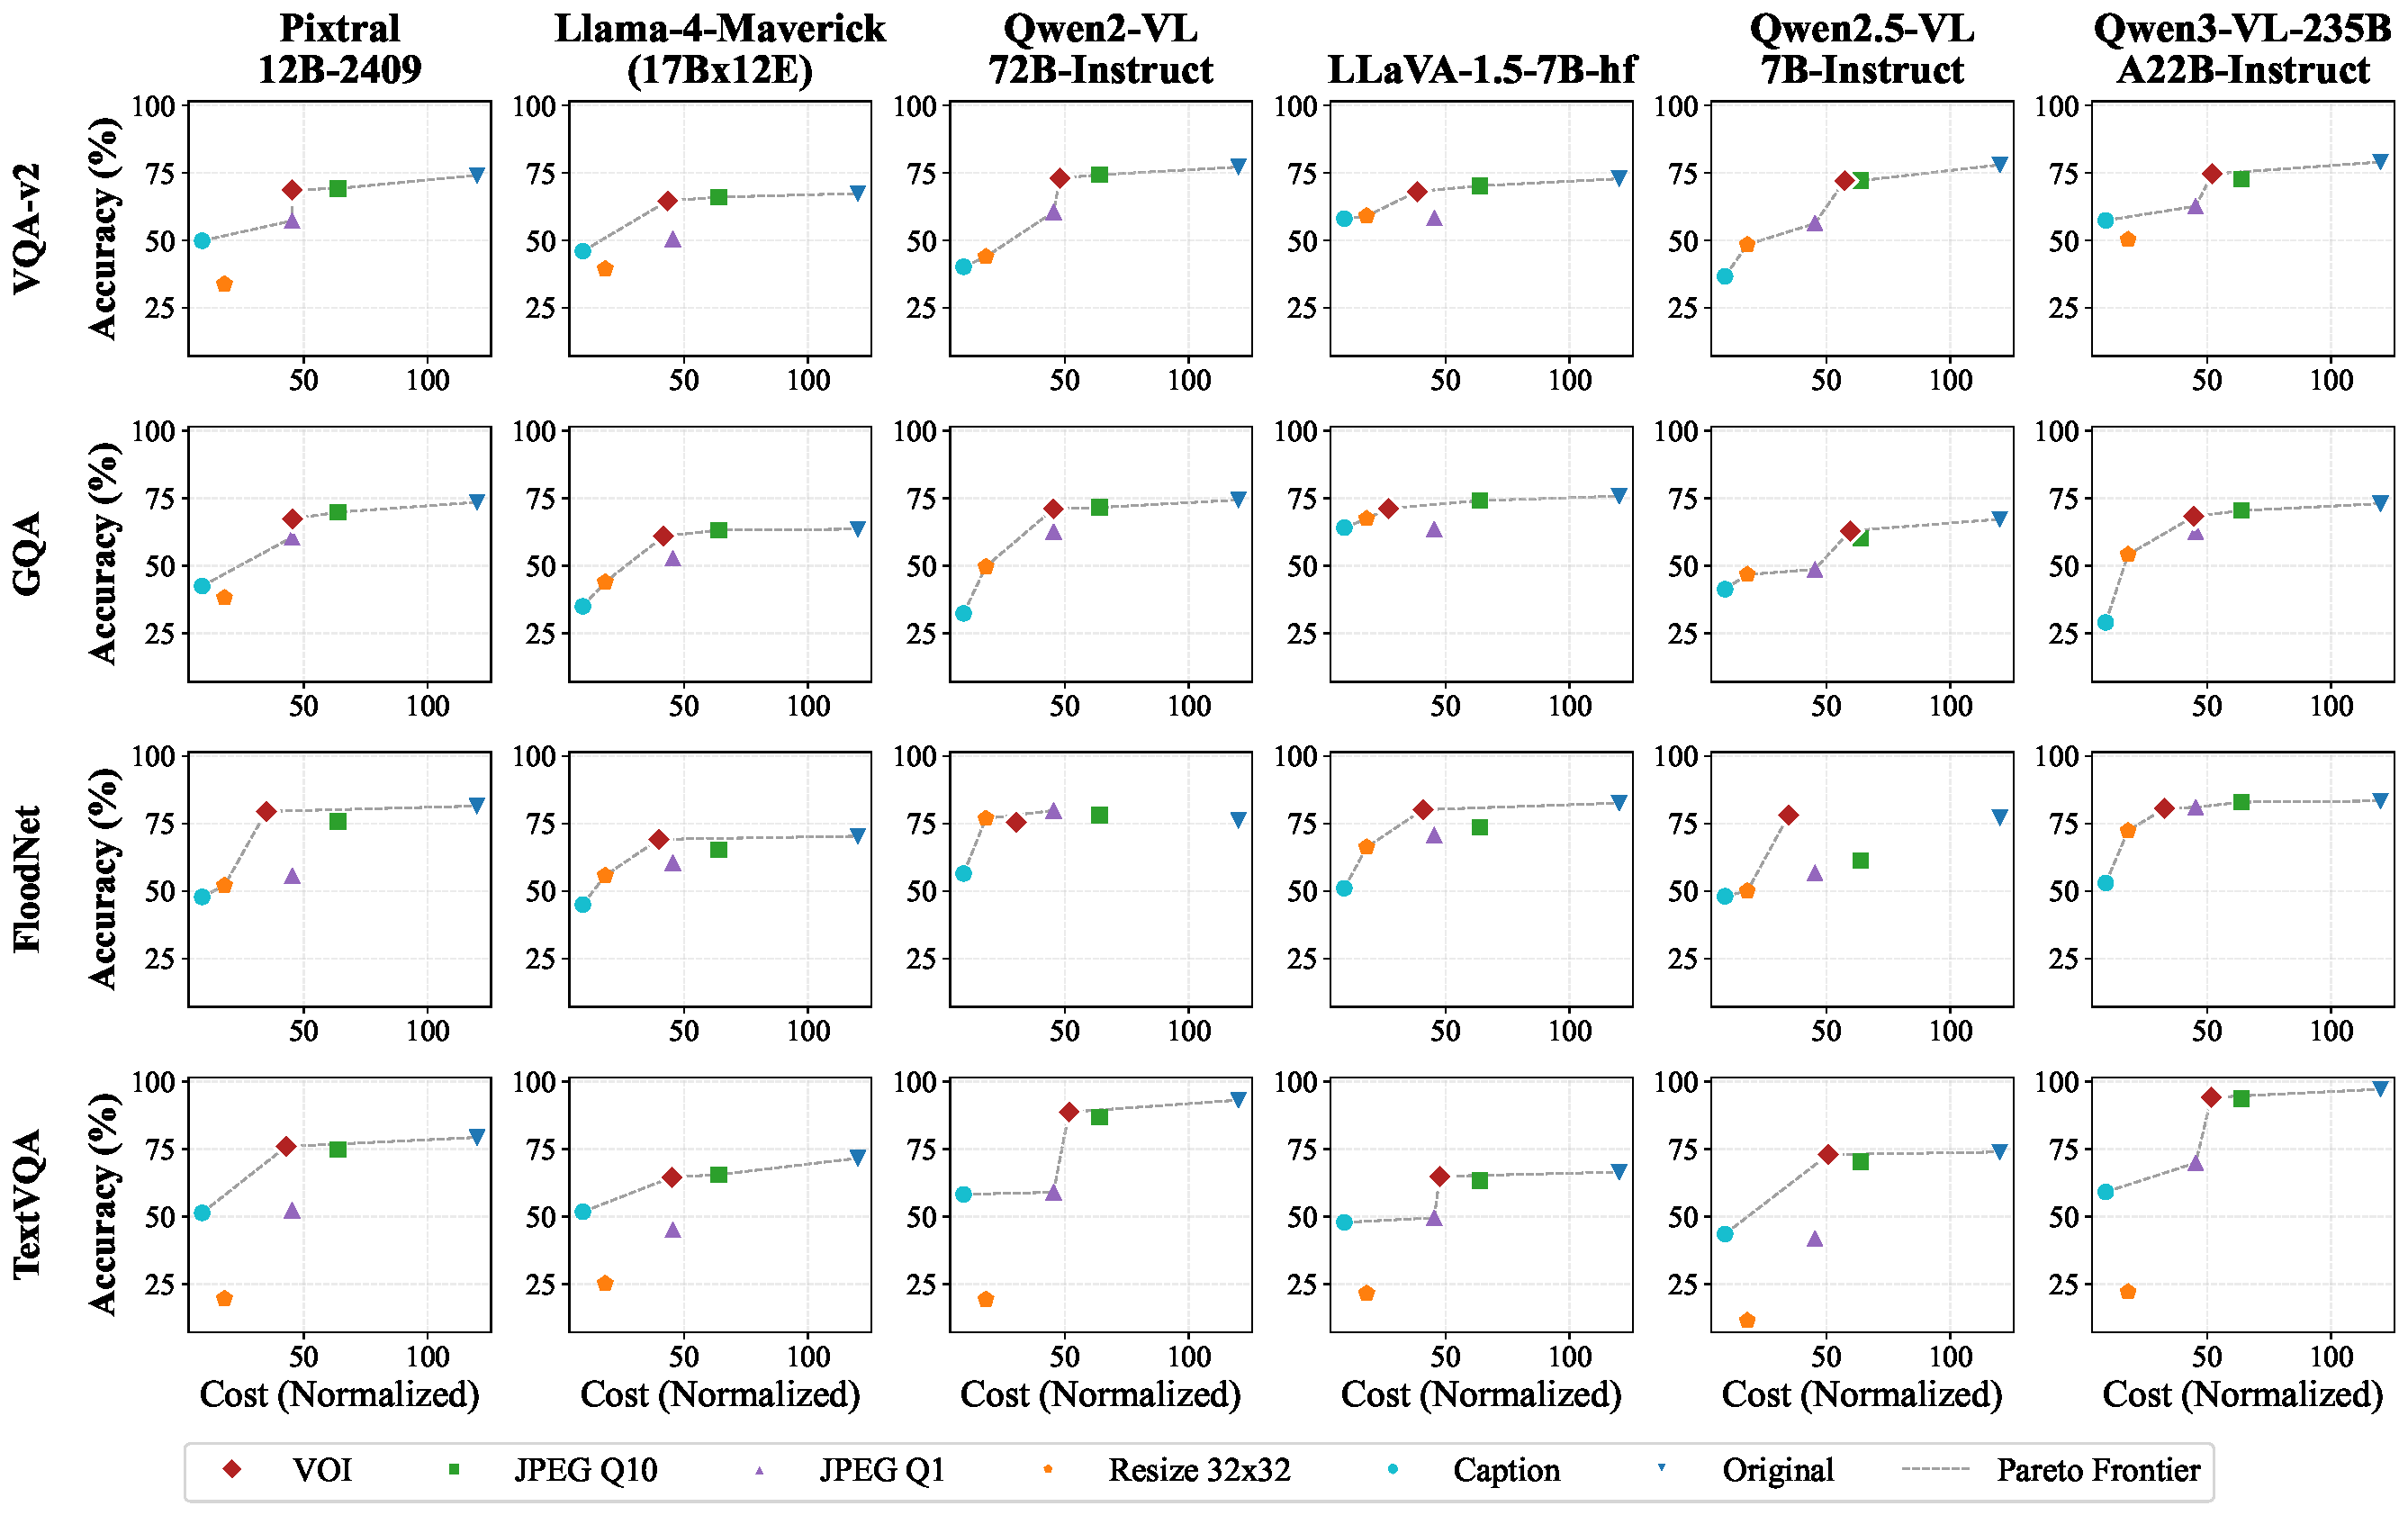
\includegraphics[width=0.95\linewidth]{plots/pareto_frontier_plot.pdf}
%     \caption{\textbf{Accuracy--cost Pareto frontiers across datasets and models.}
% Each subplot plots accuracy versus normalized retrieval cost (upper left is better) for a dataset--model pair, comparing \textsc{VOILA} to fixed-fidelity baselines, the Log-prob Cascade, the GPT-4o LLM Router, and the Oracle upper bound.
% Dashed curves denote Pareto frontiers.
% Across datasets and model scales, \textsc{VOILA} lies on or near the frontier, achieving near--full-resolution accuracy at 60--80\% lower average cost.}
%     \label{fig:pareto}
% \end{figure*}

\begin{table*}[htb]
\centering
\small
\setlength{\tabcolsep}{4pt}
\renewcommand{\arraystretch}{0.90}
\caption{\textbf{Average Acc\,(\%) and Cost across six VLMs} on four in-distribution benchmarks and LoCoMo$^\dagger$ (zero-shot OOD). Cost normalized so full-resolution $=100$; lower is better. \textsc{VOILA} rows bolded. Full per-VLM breakdown in Table~\ref{tab:complete_results} (Appendix~\ref{sec:complete_results}).}
\label{tab:master_comparison}
\resizebox{\linewidth}{!}{\begin{tabular}{@{}l rr rr rr rr rr@{}}
\toprule
& \multicolumn{2}{c}{\textbf{VQA-v2}}
& \multicolumn{2}{c}{\textbf{GQA}}
& \multicolumn{2}{c}{\textbf{TextVQA}}
& \multicolumn{2}{c}{\textbf{FloodNet}}
& \multicolumn{2}{c}{\textbf{LoCoMo}$^\dagger$} \\
\cmidrule(lr){2-3}\cmidrule(lr){4-5}\cmidrule(lr){6-7}\cmidrule(lr){8-9}\cmidrule(lr){10-11}
\textbf{Method} & Acc\% & Cost & Acc\% & Cost & Acc\% & Cost & Acc\% & Cost & Acc\% & Cost \\
\midrule
\multicolumn{11}{l}{\textit{Fixed fidelity}} \\[1pt]
Caption        & 47.8 & 7.6  & 39.9 & 7.6  & 75.7 & 7.6  & 41.8 & 7.6  & 29.6 & 7.6  \\
Full           & 75.0 & 100  & 70.2 & 100  & 86.6 & 100  & 60.1 & 100  & 59.8 & 100  \\
\midrule
\multicolumn{11}{l}{\textit{Adaptive baselines}} \\[1pt]
Log-prob Cascade   & 54.5 & 36.6 & 51.1 & 44.7 & 71.9 & 39.3 & 55.8 & 38.1 & 31.5 & 36.9 \\
GPT-4o Router      & 67.2 & 49.2 & 57.7 & 40.5 & 84.5 & 70.7 & 55.1 & 46.3 & 48.5 & 43.3 \\
BERT Router        & 62.0 & 40.9 & 59.7 & 40.9 & 71.9 & 33.1 & 59.8 & 39.2 & 47.2 & 51.8 \\
\textsc{VOILA}-CDF & 55.5 & 18.1 & 55.5 & 21.1 & 72.1 & 25.1 & 58.2 & 41.8 & \multicolumn{2}{c}{---} \\
\midrule
\multicolumn{11}{l}{\textit{Upper bound}} \\[1pt]
Oracle             & 86.9 & 29.8 & 83.5 & 33.2 & 96.7 & 18.2 & 81.5 & 35.6 & 79.0 & 41.9 \\
\midrule
\textbf{\textsc{VOILA} (ours)} & \textbf{64.9} & \textbf{35.2} & \textbf{59.6} & \textbf{27.9} & \textbf{84.8} & \textbf{26.6} & \textbf{63.5} & \textbf{19.3} & \textbf{45.1} & \textbf{36.6} \\
\bottomrule
\end{tabular}}
{\footnotesize $^\dagger$Zero-shot OOD (trained on VQA-v2+GQA); 2 VLMs only (Pixtral-12B, Qwen2.5-VL-7B). ``---'' = not evaluated.}
\end{table*}

\fablenote{Table~\ref{tab:master_comparison} issues to fix for AAAI: (1) On VQA-v2 the GPT-4o Router (67.2) beats \textsc{VOILA} (64.9) on raw accuracy --- the bolded VOILA row visually claims a win the numbers do not show. Add a matched-cost row (\textsc{VOILA} with $\lambda$ tuned to cost $\approx$49) or an accuracy-per-cost column so the table itself demonstrates dominance. (2) No variance: add bootstrap 95\% CIs or at least mark which gaps are significant. (3) The LoCoMo column averages 2 VLMs while others average 6 --- footnote this in the caption text, not only the dagger, or reviewers will catch the apples-to-oranges averaging. (4) Report the GPT-4o Router's own routing cost (one GPT-4o call per query is not free); currently its Cost column counts only retrieval, which flatters the baseline you beat and undersells your win.}

\textbf{VOILA consistently matches near-full-resolution accuracy at dramatically lower cost.}
Table~\ref{tab:master_comparison} reports per-VLM accuracy and cost for all methods across four datasets.
\textsc{VOILA} lies consistently close to the full-resolution operating point across all four datasets and all six VLMs, while operating at substantially lower retrieval cost.
Fidelity selection distributions are provided in Appendix~\ref{sec:complete_results} (Figure~\ref{fig:voila_fidelity_distribution}).
On VQA-v2, \textsc{VOILA} achieves an average accuracy of 64.9\% at an average cost of 35.1, compared to 75.0\% at cost 100 for full-resolution --- a gap of only 10.1 accuracy points while reducing retrieval cost by 65\%.
On TextVQA, the gap narrows to 1.8 accuracy points (84.8\% vs.\ 86.6\%) while reducing cost by 73\%, demonstrating that \textsc{VOILA} can almost exactly recover full-resolution performance at a fraction of the cost when caption-level text descriptions are sufficient for the dominant question types.
On FloodNet, \textsc{VOILA} (avg.\ 63.5\%) actually \emph{exceeds} fixed-cost full-resolution accuracy (avg.\ 60.1\%) while operating at less than 20\% of the full-resolution retrieval cost --- a result attributable to adaptive routing away from modalities where high-resolution imagery does not improve accuracy for this model and question distribution.
\fablenote{The first paragraph's numbers disagree with the table: text says cost 35.1 on VQA-v2, Table~\ref{tab:master_comparison} says 35.2; text says TextVQA gap 1.8 points but 86.6$-$84.8$=$1.8 at 73\% cost reduction while the table cost (26.6) implies 73.4\%. Sweep every inline number against the table before submission --- AAAI reviewers spot-check these. Also, ``adaptive routing away from modalities'' is the wrong word (fidelities, not modalities).}
Per-question-type analysis reveals the mechanism: Condition Recognition queries---the dominant FloodNet category---consistently peak at compressed fidelities across most models (e.g., Pixtral-12B at JPEG Q10: 61.9\%; LLaVA-1.5-7B at caption: 91.3\%; Qwen2-VL-72B at $32{\times}32$ resize: 98.8\%; Qwen3-VL-235B at JPEG Q1: 98.0\%), while counting queries require full resolution.
\textsc{VOILA} routes Condition Recognition queries to their optimal compressed fidelity and counting queries to full resolution, achieving higher average accuracy than the full-resolution baseline, which incurs unnecessary bandwidth cost on Condition Recognition queries without accuracy benefit.

\textbf{VOILA substantially outperforms the Log-prob Cascade and GPT-4o Router.}
The Log-prob Cascade~\cite{chen2023frugalgpt} shows highly variable performance: on VQA-v2, cascade accuracy averages 55.3\% vs.\ \textsc{VOILA}'s 64.9\%.
The cascade also exhibits systematic degeneracy (Table~\ref{tab:cascade_degeneracy}, Appendix~\ref{sec:ablations}): Qwen2-VL-72B escalates in only 0.03--0.18\% of queries (caption confidence is always high regardless of correctness), while Qwen3-VL-235B escalates in 99.96\% of GQA queries (effectively always full-resolution).
Averaged across 24 model--dataset pairs, the cascade incurs cost 39.7 vs.\ \textsc{VOILA}'s 27.3---45\% higher---confirming log-probability is an unstable escalation signal.
The GPT-4o Router achieves 66.5\% accuracy on VQA-v2 but at fixed cost 52.3; \textsc{VOILA} matches its accuracy at 33\% lower cost by exploiting structured per-query linguistic variation.

\textbf{VOILA outperforms a supervised BERT Router at lower cost.}
Despite richer question representations, the BERT Router averages 62.3\% accuracy at cost 39.3, while \textsc{VOILA} achieves 64.9\% at cost 27.3 (4.4 accuracy points higher at 30\% lower cost).
Direct fidelity label prediction has no mechanism to balance accuracy gain against retrieval cost; \textsc{VOILA}'s VOI criterion explicitly optimizes this tradeoff, confirming that cost-aware routing is the critical ingredient, not features.

\textbf{Gains persist under distribution shift and scale.}
The same Pareto improvements hold across 7B--235B models: larger models improve absolute accuracy but \textsc{VOILA}'s relative advantage remains, confirming adaptive information acquisition is complementary to model scaling.
The Oracle--\textsc{VOILA} gap decomposes into three quantifiable error modes (Pixtral-12B): over-escalation (correct answer at higher fidelity than needed) accounts for 30--41\% of queries; under-escalation (too low fidelity, wrong answer) 23--25\%; irreducible failures (no fidelity succeeds) 13--15\%.
Only 24--30\% of queries are routed to the oracle-optimal fidelity; reducing under-escalation through better calibration is the clearest path to closing this gap.
\fablenote{This error decomposition is excellent and currently buried mid-paragraph --- promote it to its own bolded paragraph (or small table) titled ``Where does VOILA fall short of the Oracle?''. Stating plainly that only 24--30\% of queries hit the oracle-optimal fidelity, then explaining why the system still wins on aggregate cost (over-escalation is cheap, under-escalation is rare), is the kind of honest self-analysis that separates A+ papers from B papers. Consider adding 2--3 qualitative example questions for each error mode.}




\textbf{Out-of-Distribution Generalization Holds.}
With $\lambda$/$\tau$ fixed to source-domain values (true zero-shot OOD), routing costs remain close to in-distribution across all six VLMs rather than collapsing to full-resolution (Table~\ref{tab:ood_pixtral_compact}).
VQA$\to$TextVQA retains 91.7\% of in-domain accuracy; GQA$\to$FloodNet 84.2\%; confirming question-type flags are the language-universal routing component while TF-IDF vocabulary degrades under larger domain shift.
\fablenote{Qwen3-VL-235B drops to 38.3\% on VQA$\to$GQA --- by far the worst cell in Table~\ref{tab:ood_pixtral_compact} and left unexplained. Either explain it (one sentence) or a reviewer will use it to argue OOD transfer is model-dependent. Also the table label says \texttt{ood\_pixtral\_compact} but the table covers all six models --- rename the label and check the caption-vs-content match.}

\begin{table}[htb]
\centering
\small
\setlength{\tabcolsep}{4pt}
\renewcommand{\arraystretch}{0.95}
\caption{\textbf{Cross-dataset transfer (zero-shot OOD).} $\lambda$/$\tau$ fixed to source-domain values; not re-tuned on target. Costs remain well below full-resolution (100) under both transfer directions.}
\label{tab:ood_pixtral_compact}
\begin{tabular}{lrrrr}
\toprule
& \multicolumn{2}{c}{\textbf{VQA$\to$GQA}} & \multicolumn{2}{c}{\textbf{GQA$\to$VQA}} \\
\cmidrule(lr){2-3}\cmidrule(lr){4-5}
\textbf{Model} & Acc\% & Cost & Acc\% & Cost \\
\midrule
Llama-4-Maverick & 46.5 & 26.0 & 52.8 & 25.5 \\
LLaVA-1.5-7B     & 65.7 & 18.6 & 65.6 & 35.6 \\
Pixtral-12B       & 54.1 & 34.4 & 58.8 & 32.0 \\
Qwen2.5-VL-7B    & 51.2 & 26.7 & 49.8 & 21.7 \\
Qwen2-VL-72B     & 51.9 & 24.4 & 53.4 & 24.5 \\
Qwen3-VL-235B    & 38.3 & 25.2 & 62.2 & 29.7 \\
\bottomrule
\end{tabular}
\end{table}

\textbf{LoCoMo and FloodNet.}
Trained only on VQAv2+GQA and evaluated zero-shot on LoCoMo, \textsc{VOILA} achieves 45.1\% accuracy at cost 36.6---63\% lower retrieval cost than full resolution (59.8\% at cost 100)---while outperforming the Log-prob Cascade by 13.6 accuracy points at similar cost (Table~\ref{tab:master_comparison}).
The cascade degenerates under domain shift: Qwen2.5-VL-7B's cascade collapses to cost 7.6 (26.9\% accuracy, caption-only), while Pixtral-12B's inflates to cost 66.1 (36.0\%)---an expected failure mode given that log-probability thresholds are calibrated to the source domain.
\textsc{VOILA}'s VOI routing, by contrast, remains stable because it depends on calibrated question features rather than post-hoc VLM confidence.
On FloodNet, \textsc{VOILA} routes Condition Recognition queries to compressed fidelities and counting queries to full resolution, achieving the highest cost savings (75--87\%), exceeding the full-resolution accuracy.


\textbf{Calibration is the central enabler of effective VOI routing.}
Isotonic calibration (in \textsc{VOILA}) consistently achieves the best accuracy--cost Pareto position across all six VLMs (Table~\ref{tab:ablation_calibration}, Appendix~\ref{sec:ablations}), reducing average acquisition cost by 10--25\% relative to uncalibrated routing while maintaining comparable accuracy.
Temperature scaling degrades both metrics, consistent with known OOD limitations~\cite{guo2017calibrationmodernneuralnetworks}.
The accuracy-only variant achieves high accuracy but at full-resolution cost (100), confirming the Pareto gain requires cost-aware routing.
Predictor ablations (Table~\ref{tab:predictor_robustness_pixtral}, Appendix~\ref{sec:ablations}) confirm that routing quality is driven by calibration rather than the predictor.

\textbf{Combining TF-IDF and structural features achieves the best cost--accuracy Pareto position.}
Table~\ref{tab:feature_ablation} ablates the feature vector on VQA-v2 with Pixtral-12B.
Question-type flags alone achieve the highest accuracy (69.1\%) but highest cost (50.5), because the five binary flags identify question category but lack vocabulary to route individual queries confidently to low fidelity.
The full TF-IDF+struct combination achieves the best Pareto position (64.1\% / 38.7): 24\% lower cost than flags-only at the cost of 5 accuracy points.
Question flags are also the language-universal component for OOD transfer (58.4\% on GQA flags-only vs.\ 52.4\% TF-IDF-only), while TF-IDF vocabulary is corpus-specific and degrades under domain shift.

\begin{table}[htb]
\centering
\small
\setlength{\tabcolsep}{4pt}
\renewcommand{\arraystretch}{0.95}
\caption{\textbf{Feature group ablation} (Pixtral-12B, VQA-v2). TF-IDF+struct is the full \textsc{VOILA} feature set; best Pareto position in bold.
\fablenote{Bolding 64.1/38.7 as ``best'' while flags-only shows 69.1/50.5 will read as self-serving: the full feature set has the LOWEST accuracy in the table. Either justify with the scalar utility metric ($\mathrm{Acc}-\lambda\cdot\mathrm{Cost}$ at the deployed $\lambda$), or report each feature set at matched cost. As written, a reviewer can argue the ablation shows your 5,012 extra features hurt accuracy.}}
\label{tab:feature_ablation}
\begin{tabular}{lrcc}
\toprule
\textbf{Feature set} & \textbf{Dims} & \textbf{Acc\%} & \textbf{Cost} \\
\midrule
TF-IDF only              & 5{,}000 & 66.1 & 45.2 \\
Question-type flags only & 5       & 69.1 & 50.5 \\
Lexical stats only       & 12      & 65.4 & 40.3 \\
TF-IDF + struct (\textsc{VOILA}) & 5{,}017 & \textbf{64.1} & \textbf{38.7} \\
\bottomrule
\end{tabular}
\end{table}

\textbf{VOILA Overheads.} \textsc{VOILA} adds 0.45\,ms per query on CPU (0.04\,MB memory), compared to 2.4--62.8\,s for VLM inference; training takes 21\,s per configuration. Full profiling is in Appendix~\ref{sec:computational_overhead}.


\section{Related Work}\label{sec:related}

\noindent\textbf{VQA and pre-retrieval query difficulty.}
VQA~\cite{antol2015vqa,goyal2017vqav2,hudson2019gqa,singh2019textvqa} established that question type strongly predicts difficulty~\cite{kafle2017analysis,agrawal2018dont}.
Estimating retrieval quality from query features alone---without executing retrieval---is a classic IR problem~\cite{zhao2008predicting,hauff2008improved,mothe2005linguistic}; \textsc{VOILA} applies this paradigm cross-modally.
\textbf{Post-retrieval cascades and model routing.}
FrugalGPT~\cite{chen2023frugalgpt} and RouteLLM~\cite{wang2024routellm} reduce cost by routing \emph{after} context is fetched; early-exit transformers~\cite{zhou2020bert,schuster2022confident} skip layers for easy inputs.
All assume fully-retrieved context; \textsc{VOILA} selects \emph{which} context to acquire before any retrieval.
\textbf{Adaptive visual resolution.}
CARES~\cite{kimhi2025cares} selects resolution using a compact VLM on the already-retrieved image; \textsc{VOILA} operates strictly from question text---no image access at decision time.
\textbf{VOI and multimodal RAG.}
The VOI framework~\cite{bilgic2011value} formalizes information acquisition under cost; multimodal RAG~\cite{lewis2020rag,yasunaga2023retrievalaugmented,chen2022murag} treats retrieval as binary at fixed quality---\textsc{VOILA} introduces fidelity as a continuous retrieval axis.
Extended discussion of all related work threads is in Appendix~\ref{sec:related_ext}.
\fablenote{For AAAI, two gaps in related-work coverage: (1) cost-sensitive / active feature acquisition (e.g., Greiner et al.\ 2002; Shim et al.\ 2018 ``Joint Active Feature Acquisition and Classification'') --- this is the AAAI-native literature VOILA belongs to, and omitting it invites ``missing related work'' from exactly this venue's reviewers; (2) visual token compression / AnyRes-style adaptive resolution in modern VLMs (LLaVA-NeXT AnyRes, token-pruning work) --- distinct from VOILA (post-retrieval, image-dependent) but close enough that a reviewer will expect the distinction drawn explicitly. The IR query-difficulty thread, prominent in the EMNLP framing, can be compressed to one clause here to make room.}

% -----------------------------------------------------------------------
% REWRITTEN conclusion — expanded to ~12 lines; NLP thesis bookend;
% future work; dataset release; \expnote for pending items
% -----------------------------------------------------------------------

\section{Conclusion}

Question linguistic structure is a principled and practical signal for pre-retrieval fidelity selection: \emph{how many}, \emph{what color}, and \emph{read the text} reliably require high-resolution evidence, while \emph{is there} and \emph{what type} are resolvable from low-fidelity representations.
\textsc{VOILA} operationalizes this insight via a gradient-boosted classifier, isotonic calibration, and a greedy value-of-information decision rule---selecting the minimum-cost sufficient fidelity from question text alone, before any image is accessed---reducing retrieval cost by 50--65\% across five datasets and six VLMs (7B--235B parameters) while matching or exceeding full-resolution accuracy on OCR-heavy and domain-specialized benchmarks, and remaining within an average of 10 accuracy points on general VQA.
Natural extensions include richer question encoders for ambiguous queries, multilingual support, and fidelity selection for video (frame rate) and document retrieval (chunk size); code, checkpoints, and the LoCoMo-VQA benchmark will be released.
\fablenote{For AAAI, close on the decision-theoretic thesis rather than the linguistic one: e.g., ``More broadly, VOILA demonstrates that the value of information an AI system acquires can be estimated before paying for it --- a principle that extends beyond images to any perception pipeline with tiered acquisition costs.'' This bookends the AAAI framing suggested for the abstract and positions the paper as a general contribution to resource-bounded AI rather than a VQA-specific trick. Also reconcile ``50--65\%'' here with whichever range the abstract settles on.}


% Required by ACL ARR — does not count toward the page limit
\section*{Limitations}
\label{sec:limitations}

\fablenote{Every limitation below is immediately neutralized with a ``but this is easy to fix'' clause, which reads as spin. A+ practice: state at least one limitation plainly and without rebuttal --- the honest one here is the 10-point average accuracy gap on general VQA and the fact that only 24--30\% of queries are routed oracle-optimally. Adding ``\textbf{Accuracy gap on general VQA.}'' as the first item, stated neutrally, will increase reviewer trust in everything else. Note AAAI does not mandate this section; if space is tight, fold it into the conclusion --- but keep the honest accuracy-gap item wherever it lands.}

\textbf{Discrete fidelity set.}
\textsc{VOILA} is designed for the discrete fidelity tiers that characterize real-world tiered storage (captions, thumbnails, compressed JPEGs, full resolution).
Extending the VOI rule to continuous compression schemes is a natural next step that would replace the piecewise policy with a continuous acquisition function.

\textbf{Per-VLM calibration.}
The gradient-boosted regressor is calibrated on correctness labels from a specific VLM.
Collecting these labels is lightweight---3{,}000--12{,}000 examples per configuration suffice---and needs to be done only once offline per VLM--dataset pair.
Cross-model transfer and few-shot calibration are promising directions for model-as-a-service settings.

\textbf{English-language features.}
The current TF-IDF vocabulary and question-type rules target English VQA.
The structural features (question-type flags, lexical patterns) are language-portable, and multilingual extension via language-agnostic encoders is straightforward given labeled data.

\textbf{Synthetic LoCoMo annotations.}
\providecommand{\locomotableref}{\ref{tab:locomo_ultracompact_appendix}}
LoCoMo questions and reference answers are generated by GPT-4o; we use this dataset as an out-of-distribution stress test rather than a primary benchmark, and the strong zero-shot transfer results (Table~\locomotableref) suggest the approach is robust to annotation noise.

\textbf{Cost model grounding.}
The retrieval cost function is derived from empirical file-size ratios and standard tier-latency profiles.
Adapting to a specific deployment requires only re-measuring file sizes and tier latencies---the VOI decision rule is otherwise unchanged.

\textbf{Scope: image VQA.}
\textsc{VOILA} is evaluated on image-based VQA; the VOI framework is modality-agnostic, and applying pre-retrieval fidelity selection to video (temporal sampling), audio (bitrate), and document retrieval (chunk granularity) is a direct extension.


% Optional ethical considerations — does not count toward the page limit
\section*{Ethical Considerations}

\textsc{VOILA} enables cost-aware multimodal inference in edge-cloud VQA systems (mobile assistants, photo search), agentic memory systems with tiered storage, and mission-critical cyber-physical applications (disaster response drones, IoT monitoring).
By achieving 50--60\% retrieval cost reductions within 2--6 accuracy points of full-resolution baselines, \textsc{VOILA} can substantially reduce energy consumption and bandwidth usage in production systems while enabling deployment in resource-constrained settings previously infeasible due to cost or latency requirements.

Efficiency gains improve sustainability and accessibility of multimodal AI---lowering carbon footprint and expanding access in bandwidth-limited contexts.
However, \textsc{VOILA} relies on learned predictors that may reflect dataset biases.
Inaccurate calibration could cause under-retrieval of critical information in high-stakes scenarios.
A concrete example of potential disparity: because our training data (VQA-v2, GQA) consists predominantly of Western images with Latin-script text, the TF-IDF vocabulary and question-type rules may systematically underestimate the visual fidelity required for OCR-dependent queries in non-Latin scripts (e.g., Arabic, Chinese, Devanagari).
A user querying \emph{``What does the sign say?''} about an Arabic-script sign may be routed to a lower fidelity than necessary, degrading accuracy for that population.
Our experiments use English-language benchmarks; generalization to other languages and visual contexts requires separate validation and targeted retraining.

Key mitigation directions include: (1) developing calibration methods with formal safety guarantees, (2) evaluating performance across diverse populations and domains to identify disparate impacts, and (3) extending the framework to jointly optimize cost, accuracy, and fairness.
Practitioners should monitor calibration quality continuously, validate on domain-specific data before deployment, and maintain human oversight for high-stakes decisions.
We will release our code, trained GBR checkpoints, and the LoCoMo-VQA benchmark to enable community scrutiny and responsible extension of this work.

% Note: acl.sty already calls \bibliographystyle{acl_natbib} internally.
% Calling it again here causes a duplicate \bibstyle in the .aux file (BibTeX error).
\bibliography{example_paper}

%%%%%%%%%%%%%%%%%%%%%%%%%%%%%%%%%%%%%%%%%%%%%%%%%%%%%%%%%%%%%%%%%%%%%%%%%%%%%%%
% APPENDIX
%%%%%%%%%%%%%%%%%%%%%%%%%%%%%%%%%%%%%%%%%%%%%%%%%%%%%%%%%%%%%%%%%%%%%%%%%%%%%%%
\newpage
\onecolumn
\appendix

\section*{Appendices}
\addcontentsline{toc}{section}{Appendices}

\renewcommand{\thesubsection}{\Alph{section}.\arabic{subsection}}

\begin{center}
\textbf{\Large Table of Contents}
\end{center}

\vspace{1em}

\noindent\textbf{Appendix~\ref{sec:complete_results}: Complete Results} \dotfill \pageref{sec:complete_results}
\begin{itemize}[leftmargin=2em, label={}]
    \item \ref{sec:complete_tables} Complete Accuracy and Cost Tables \dotfill \pageref{sec:complete_tables}
    \item \ref{sec:fidelity_distributions} Fidelity Selection Distributions \dotfill \pageref{sec:fidelity_distributions}
\end{itemize}

\vspace{0.5em}

\noindent\textbf{Appendix~\ref{sec:datasets}: Dataset Details} \dotfill \pageref{sec:datasets}
\begin{itemize}[leftmargin=2em, label={}]
    \item \ref{sec:vqa_datasets} VQA-v2, GQA, and TextVQA \dotfill \pageref{sec:vqa_datasets}
    \item \ref{sec:floodnet} FloodNet \dotfill \pageref{sec:floodnet}
    \item \ref{sec:locomo} LoCoMo Question Generation \dotfill \pageref{sec:locomo}
\end{itemize}

\vspace{0.5em}

\noindent\textbf{Appendix \ref{sec:theory}: Theoretical Foundations} \dotfill \pageref{sec:theory}
\begin{itemize}[leftmargin=2em, label={}]
    \item \ref{sec:bayes_optimal} Bayes-Optimal Fidelity Selector \dotfill \pageref{sec:bayes_optimal}
    \item \ref{sec:calibration} Learning Utility via Calibration \dotfill \pageref{sec:calibration}
    \item \ref{sec:optimality} Optimality Under Perfect Calibration \dotfill \pageref{sec:optimality}
    \item \ref{sec:regret} Regret with Imperfect Calibration \dotfill \pageref{sec:regret}
    \item \ref{sec:generalization} Generalization to Unseen Questions \dotfill \pageref{sec:generalization}
    \item \ref{sec:greedy_policy} Sequential Greedy Policy \dotfill \pageref{sec:greedy_policy}
    \item \ref{sec:implications} Implications for Adaptive Fidelity Selection \dotfill \pageref{sec:implications}
    \item \ref{sec:theory_empirics} Connection to Empirical Observations \dotfill \pageref{sec:theory_empirics}
\end{itemize}

\vspace{0.5em}

\noindent\textbf{Appendix D: Cost Model Details} \dotfill \pageref{sec:cost_model}
\begin{itemize}[leftmargin=2em, label={}]
    \item \ref{sec:fidelity_set} Fidelity Set \dotfill \pageref{sec:fidelity_set}
    \item \ref{sec:bandwidth} Empirical Bandwidth Proxy \dotfill \pageref{sec:bandwidth}
    \item \ref{sec:tier_cost} Tier-Aware Acquisition Cost \dotfill \pageref{sec:tier_cost}
    \item \ref{sec:normalization} Normalization \dotfill \pageref{sec:normalization}
    \item \ref{sec:deployment} Deployment Profiles \dotfill \pageref{sec:deployment}
    \item \ref{sec:measurement} Empirical Measurement Procedure \dotfill \pageref{sec:measurement}
    \item \ref{sec:sensitivity} Sensitivity Analysis \dotfill \pageref{sec:sensitivity}
\end{itemize}

\vspace{0.5em}

\noindent\textbf{Appendix E: Experimental Details} \dotfill \pageref{sec:experimental}
\begin{itemize}[leftmargin=2em, label={}]
    \item \ref{sec:features} Question Feature Extraction \dotfill \pageref{sec:features}
    \item \ref{sec:hyperparams} Calibration Model and Hyperparameters \dotfill \pageref{sec:hyperparams}
    \item \ref{sec:cross_validation} Cross-Validation Protocol \dotfill \pageref{sec:cross_validation}
    \item \ref{sec:voi_policy} VOI Policy and Threshold Selection \dotfill \pageref{sec:voi_policy}
    \item \ref{sec:hyperparam_search} Hyperparameter Search \dotfill \pageref{sec:hyperparam_search}
    \item \ref{sec:variance} Variance and Reporting \dotfill \pageref{sec:variance}
    \item \ref{sec:computational_overhead} Computational Overhead \dotfill \pageref{sec:computational_overhead}
\end{itemize}

\vspace{0.5em}

\noindent\textbf{Appendix F: Extended Ablation Studies} \dotfill \pageref{sec:ablations}
\begin{itemize}[leftmargin=2em, label={}]
    \item \ref{sec:ablation_design} Experimental Design \dotfill \pageref{sec:ablation_design}
    \item \ref{sec:ablation_results} Comprehensive Results \dotfill \pageref{sec:ablation_results}
    \item \ref{sec:voi_dominance} Why VOI Routing Dominates \dotfill \pageref{sec:voi_dominance}
    \item \ref{sec:predictor_robustness} Robustness to Predictor Architecture \dotfill \pageref{sec:predictor_robustness}
    \item \ref{sec:takeaways} Key Takeaways and Design Implications \dotfill \pageref{sec:takeaways}
\end{itemize}

\vspace{0.5em}

\noindent\textbf{Appendix G: Extended Related Work} \dotfill \pageref{sec:related_ext}

\vspace{2em}
\clearpage

\section{Complete Results}
\label{sec:complete_results}


\subsection{Complete Accuracy and Cost Tables}
\label{sec:complete_tables}

\begin{table*}[htbp]
\centering
\tiny
\caption{
\textbf{Complete Comparison Table (VQA-v2, GQA, FloodNet, TextVQA).}
Accuracy (\%) and average normalized acquisition cost for each method across datasets and models.
Full-resolution cost $c(\texttt{full})=100$; all other costs are normalized relative to this value.
\textsc{VOILA}-CDF uses a CDF-based threshold in place of the VOI criterion.
\textbf{\textsc{VOILA}} rows are bolded.
}
\label{tab:complete_results_vqa_gqa_flood_textvqa}\label{tab:complete_results}
\resizebox{\linewidth}{!}{
\begin{tabular}{llcccccccc}
\toprule
\multirow{2}{*}{\textbf{Model}} & \multirow{2}{*}{\textbf{Method}}
& \multicolumn{2}{c}{\textbf{VQA-v2}}
& \multicolumn{2}{c}{\textbf{GQA}}
& \multicolumn{2}{c}{\textbf{FloodNet}}
& \multicolumn{2}{c}{\textbf{TextVQA}} \\
\cmidrule(lr){3-4}\cmidrule(lr){5-6}\cmidrule(lr){7-8}\cmidrule(lr){9-10}
& & \textbf{Acc} & \textbf{Cost}
& \textbf{Acc} & \textbf{Cost}
& \textbf{Acc} & \textbf{Cost}
& \textbf{Acc} & \textbf{Cost} \\
\midrule

\multirow{9}{*}{Pixtral-12B-2409}
& Caption              & 49.5 & 7.6   & 42.1 & 7.6   & 21.3 & 7.6   & 78.0 & 7.6   \\
& Resize $32{\times}32$& 33.3 & 15.1  & 37.7 & 15.1  & 25.8 & 15.1  & 18.7 & 15.1  \\
& JPEG Q1              & 57.1 & 37.8  & 59.8 & 37.8  & 30.6 & 37.8  & 25.2 & 37.8  \\
& JPEG Q10             & 70.6 & 53.2  & 68.2 & 53.2  & 45.0 & 53.2  & 46.1 & 53.2  \\
& Full                 & 74.2 & 100.0 & 71.1 & 100.0 & 39.0 & 100.0 & 57.1 & 100.0 \\
& Log-prob Cascade     & 54.0 & 51.9  & 54.9 & 57.7  & 45.2 & 72.3  & 58.4 & 46.3  \\
& \textsc{VOILA}-CDF   & 53.0 & 21.7  & 54.2 & 18.9  & 39.7 & 35.9  & 64.6 & 28.0  \\
& Oracle               & 87.3 & 30.5  & 84.8 & 32.3  & 77.1 & 47.8  & 91.3 & 21.1  \\
& \textbf{\textsc{VOILA}} & \textbf{64.1} & \textbf{38.8} & \textbf{60.5} & \textbf{31.1} & \textbf{45.2} & \textbf{20.7} & \textbf{77.8} & \textbf{8.2} \\
\midrule

\multirow{9}{*}{Llama-4-Maverick (17Bx12E)}
& Caption              & 45.6 & 7.6   & 34.6 & 7.6   & 42.1 & 7.6   & 75.9 & 7.6   \\
& Resize $32{\times}32$& 39.7 & 15.1  & 43.2 & 15.1  & 29.9 & 15.1  & 18.9 & 15.1  \\
& JPEG Q1              & 51.2 & 37.8  & 50.7 & 37.8  & 54.4 & 37.8  & 67.7 & 37.8  \\
& JPEG Q10             & 66.3 & 53.2  & 60.8 & 53.2  & 62.8 & 53.2  & 89.3 & 53.2  \\
& Full                 & 68.4 & 100.0 & 62.9 & 100.0 & 59.7 & 100.0 & 93.7 & 100.0 \\
& Log-prob Cascade     & 45.6 & 7.9   & 34.7 & 7.7   & 41.5 & 11.8  & 75.5 & 10.6  \\
& \textsc{VOILA}-CDF   & 50.3 & 16.9  & 48.8 & 20.4  & 58.8 & 41.9  & 71.7 & 22.3  \\
& Oracle               & 82.4 & 34.3  & 77.9 & 38.7  & 84.0 & 34.9  & 98.1 & 17.7  \\
& \textbf{\textsc{VOILA}} & \textbf{59.7} & \textbf{37.1} & \textbf{53.4} & \textbf{29.5} & \textbf{61.9} & \textbf{19.1} & \textbf{86.4} & \textbf{35.6} \\
\midrule

\multirow{9}{*}{Qwen2-VL-72B-Instruct}
& Caption              & 40.2 & 7.6   & 30.8 & 7.6   & 30.7 & 7.6   & 73.3 & 7.6   \\
& Resize $32{\times}32$& 44.7 & 15.1  & 47.9 & 15.1  & 73.8 & 15.1  & 22.2 & 15.1  \\
& JPEG Q1              & 60.6 & 37.8  & 61.6 & 37.8  & 23.5 & 37.8  & 66.0 & 37.8  \\
& JPEG Q10             & 74.7 & 53.2  & 71.2 & 53.2  & 39.8 & 53.2  & 92.1 & 53.2  \\
& Full                 & 77.6 & 100.0 & 73.5 & 100.0 & 58.6 & 100.0 & 97.1 & 100.0 \\
& Log-prob Cascade     & 40.2 & 7.7   & 30.8 & 7.6   & 70.2 & 59.9  & 73.3 & 7.6   \\
& \textsc{VOILA}-CDF   & 50.5 & 16.3  & 53.6 & 23.0  & 61.5 & 52.6  & 73.3 & 26.3  \\
& Oracle               & 87.3 & 30.9  & 84.7 & 33.7  & 86.3 & 29.4  & 99.2 & 17.5  \\
& \textbf{\textsc{VOILA}} & \textbf{64.4} & \textbf{37.3} & \textbf{60.0} & \textbf{28.9} & \textbf{73.4} & \textbf{13.0} & \textbf{86.9} & \textbf{33.1} \\
\midrule

\multirow{9}{*}{LLaVA-1.5-7B-hf}
& Caption              & 57.7 & 7.6   & 63.2 & 7.6   & 67.0 & 7.6   & 79.0 & 7.6   \\
& Resize $32{\times}32$& 59.5 & 15.1  & 66.4 & 15.1  & 66.7 & 15.1  & 26.0 & 15.1  \\
& JPEG Q1              & 58.3 & 37.8  & 62.9 & 37.8  & 48.7 & 37.8  & 57.9 & 37.8  \\
& JPEG Q10             & 70.7 & 53.2  & 72.2 & 53.2  & 69.4 & 53.2  & 72.7 & 53.2  \\
& Full                 & 73.1 & 100.0 & 74.1 & 100.0 & 67.3 & 100.0 & 75.7 & 100.0 \\
& Log-prob Cascade     & 62.7 & 35.6  & 69.3 & 36.5  & 66.9 & 12.4  & 75.9 & 42.9  \\
& \textsc{VOILA}-CDF   & 62.9 & 14.6  & 68.0 & 19.0  & 68.9 & 22.9  & 69.3 & 22.5  \\
& Oracle               & 86.6 & 26.1  & 87.3 & 24.3  & 77.5 & 30.9  & 92.7 & 18.9  \\
& \textbf{\textsc{VOILA}} & \textbf{66.5} & \textbf{26.2} & \textbf{69.5} & \textbf{25.9} & \textbf{68.6} & \textbf{15.2} & \textbf{79.2} & \textbf{9.4} \\
\midrule

\multirow{9}{*}{Qwen2.5-VL-7B-Instruct}
& Caption              & 35.9 & 7.6   & 39.7 & 7.6   & 35.3 & 7.6   & 71.8 & 7.6   \\
& Resize $32{\times}32$& 48.7 & 15.1  & 45.9 & 15.1  & 50.1 & 15.1  & 23.8 & 15.1  \\
& JPEG Q1              & 57.0 & 37.8  & 47.4 & 37.8  & 55.5 & 37.8  & 64.6 & 37.8  \\
& JPEG Q10             & 72.6 & 53.2  & 59.0 & 53.2  & 63.5 & 53.2  & 92.2 & 53.2  \\
& Full                 & 77.8 & 100.0 & 66.2 & 100.0 & 62.1 & 100.0 & 97.7 & 100.0 \\
& Log-prob Cascade     & 61.4 & 74.7  & 52.0 & 74.8  & 53.2 & 51.2  & 71.1 & 64.1  \\
& \textsc{VOILA}-CDF   & 53.0 & 21.1  & 53.1 & 24.2  & 50.4 & 35.6  & 75.2 & 26.6  \\
& Oracle               & 88.0 & 31.7  & 82.5 & 36.2  & 78.5 & 39.4  & 99.3 & 18.0  \\
& \textbf{\textsc{VOILA}} & \textbf{63.1} & \textbf{34.1} & \textbf{55.0} & \textbf{27.8} & \textbf{56.6} & \textbf{22.8} & \textbf{88.2} & \textbf{38.0} \\
\midrule

\multirow{9}{*}{Qwen3-VL-235B-A22B-Instruct}
& Caption              & 57.7 & 7.6   & 29.0 & 7.6   & 54.6 & 7.6   & 75.9 & 7.6   \\
& Resize $32{\times}32$& 50.4 & 15.1  & 53.3 & 15.1  & 31.3 & 15.1  & 23.9 & 15.1  \\
& JPEG Q1              & 63.7 & 37.8  & 62.3 & 37.8  & 67.5 & 37.8  & 72.2 & 37.8  \\
& JPEG Q10             & 76.9 & 53.2  & 70.3 & 53.2  & 77.5 & 53.2  & 95.1 & 53.2  \\
& Full                 & 79.1 & 100.0 & 73.2 & 100.0 & 74.1 & 100.0 & 98.5 & 100.0 \\
& Log-prob Cascade     & 62.8 & 41.8  & 65.0 & 83.8  & 57.8 & 20.9  & 77.2 & 64.4  \\
& \textsc{VOILA}-CDF   & 63.3 & 17.7  & 55.4 & 21.2  & 70.1 & 62.1  & 78.2 & 24.9  \\
& Oracle               & 89.7 & 25.5  & 83.8 & 34.0  & 85.4 & 31.3  & 99.7 & 15.9  \\
& \textbf{\textsc{VOILA}} & \textbf{71.5} & \textbf{37.4} & \textbf{59.0} & \textbf{24.4} & \textbf{75.1} & \textbf{25.1} & \textbf{90.4} & \textbf{35.0} \\
\bottomrule
\end{tabular}
}
\end{table*}


\subsection{Fidelity Selection Distributions}
\label{sec:fidelity_distributions}

\begin{figure*}[t]
    \centering
    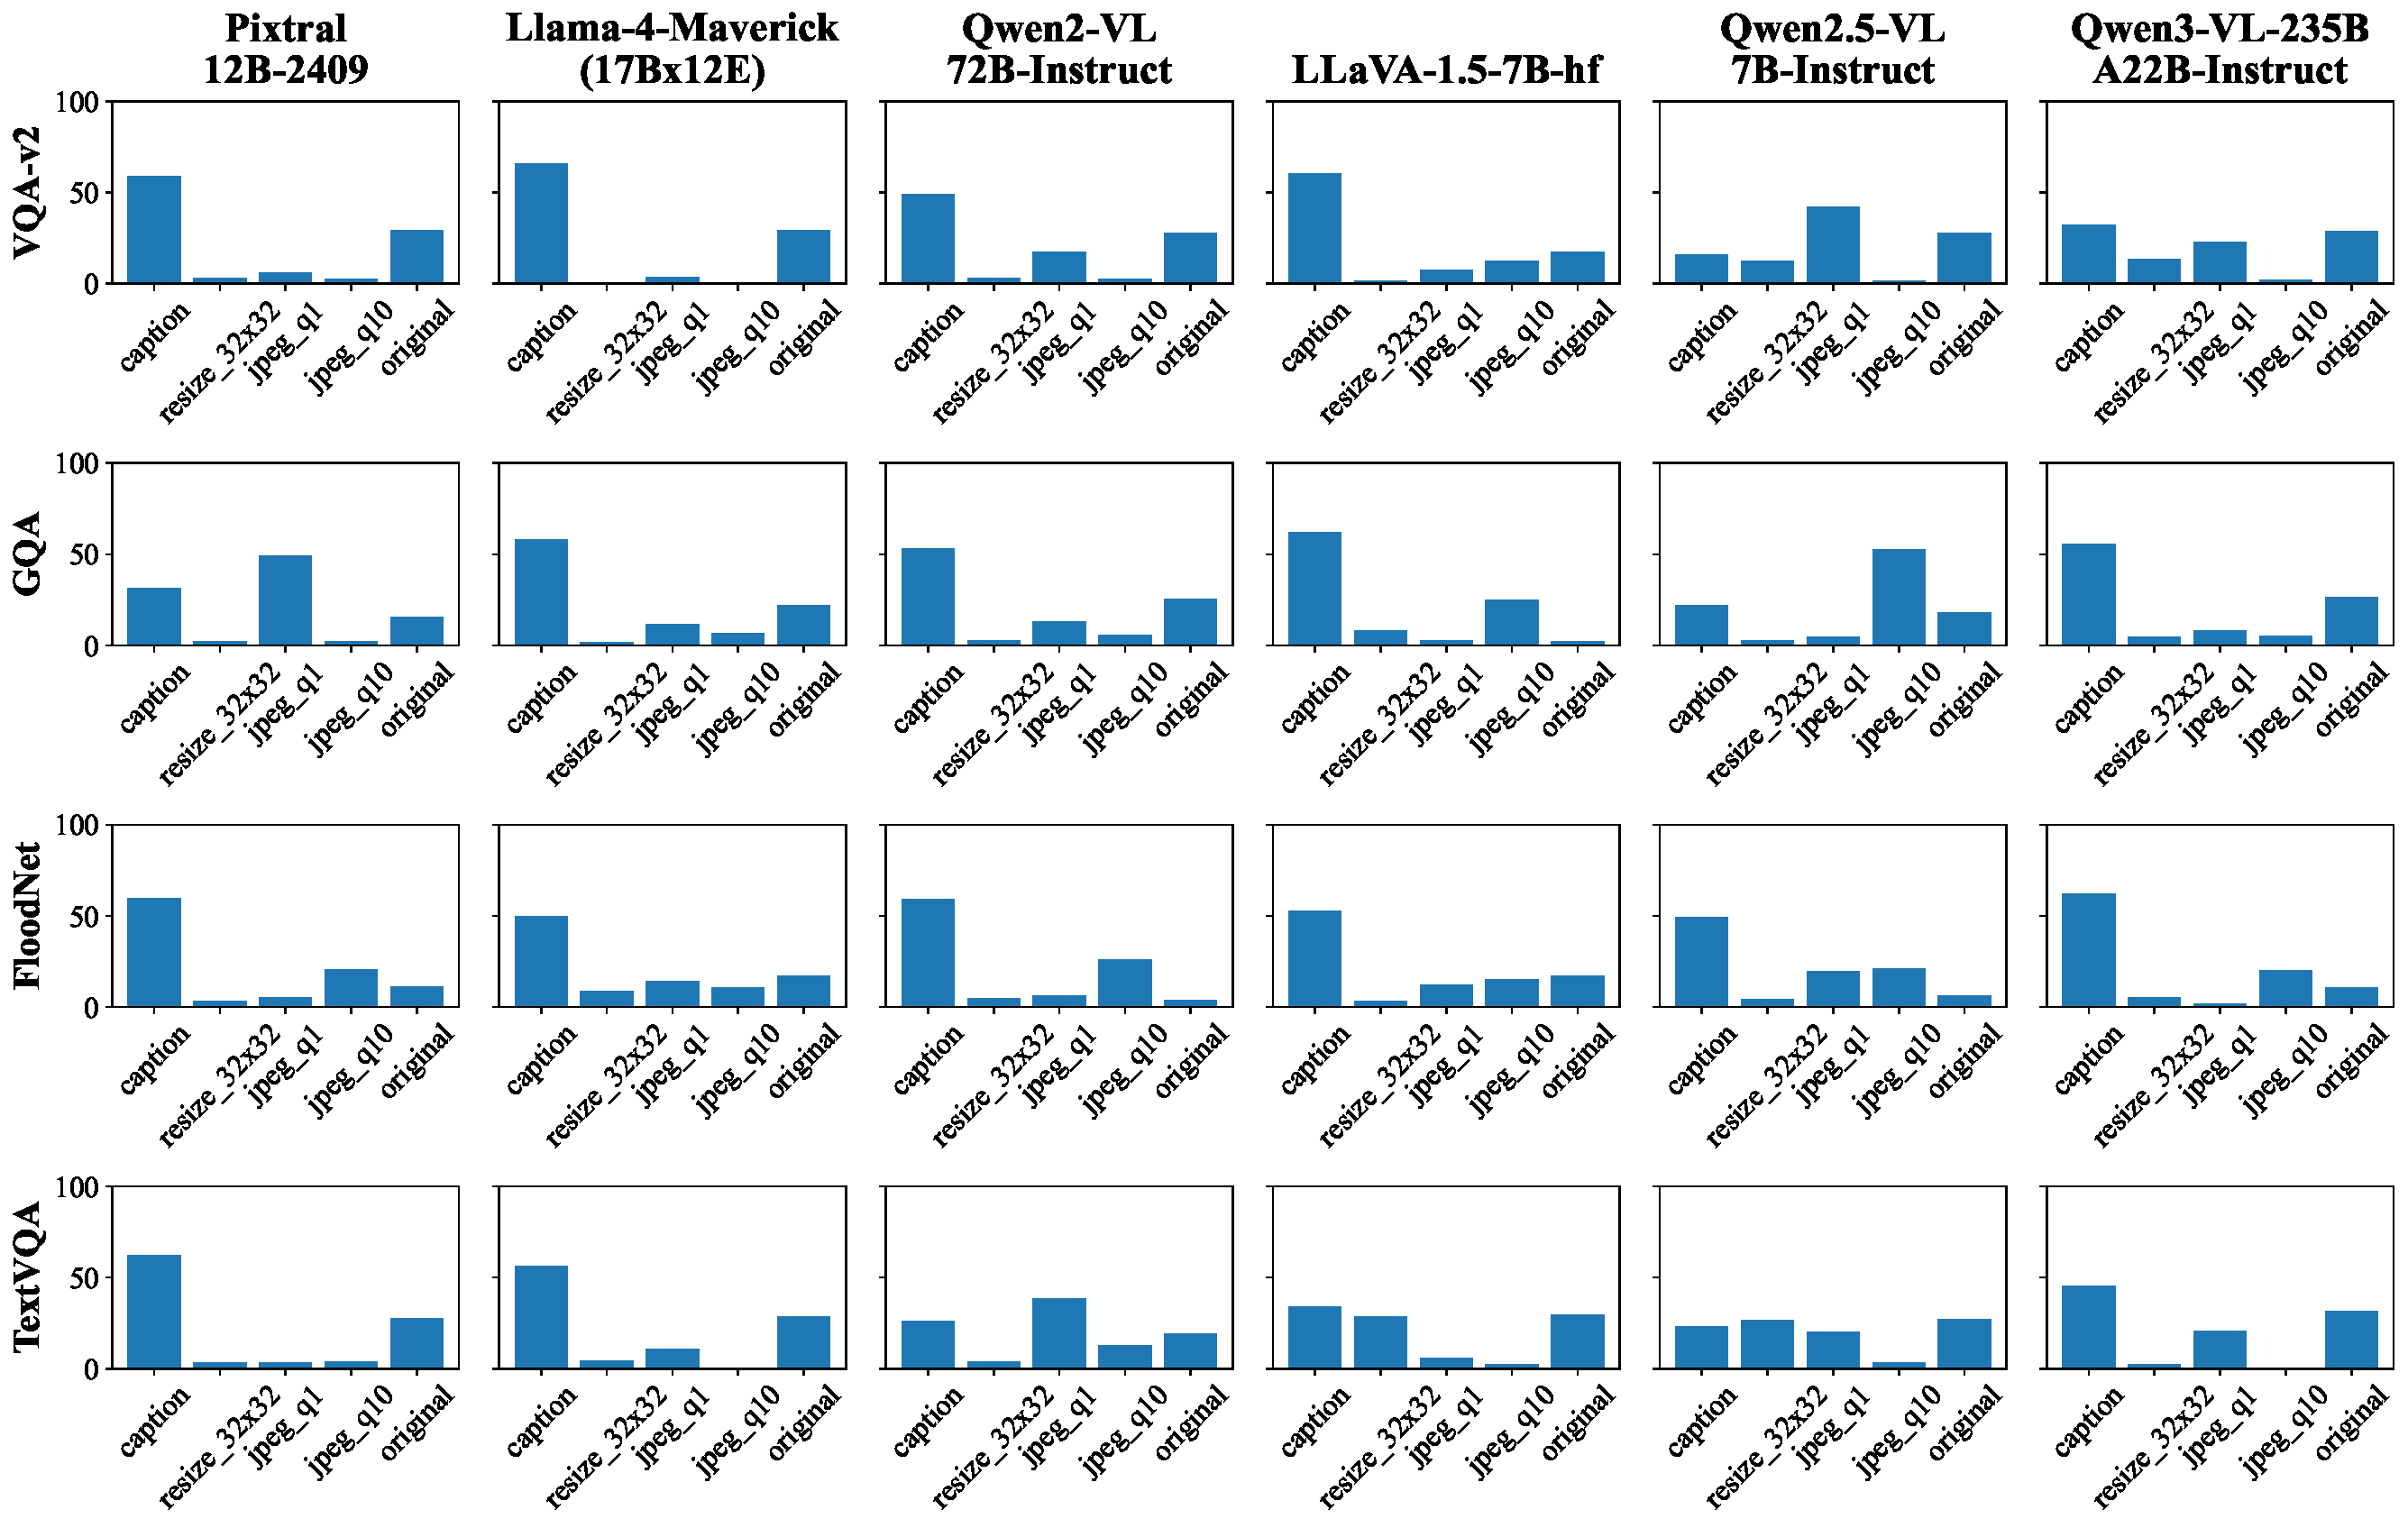
\includegraphics[width=\linewidth]{plots/fidelity_distribution_plot.pdf}
    \caption{
    \textbf{Learned fidelity selection distributions under \textsc{VOILA} routing.}
    Each subplot reports the percentage of queries routed to each input fidelity by \textsc{VOILA}, across four datasets (rows) and six vision--language models (columns).
    Low-cost representations (captions and low-resolution thumbnails) dominate across all settings, while higher-cost fidelities (JPEG Q1/Q10 and full-resolution images) are selected selectively when expected utility justifies their acquisition cost.
    }
    \label{fig:voila_fidelity_distribution}
\end{figure*}


\subsection{LoCoMo Memory Recall Results}

\begin{table}[htb]
\centering
\small
\setlength{\tabcolsep}{4pt}
\caption{\textbf{LoCoMo memory recall (Acc\% / Cost).}
\textsc{VOILA} trained on VQA-v2+GQA, evaluated on LoCoMo (OOD). Limited to two VLMs due to GPT-4o answer-generation cost.
}
\label{tab:locomo_ultracompact_appendix}
\resizebox{\columnwidth}{!}{
\begin{tabular}{lccccc}
\toprule
\textbf{Model} & \textbf{Caption} & \textbf{Full} & \textbf{BERT Router} & \textbf{LLM Router} & \textbf{\textsc{VOILA}} \\
\midrule
Pixtral-12B    & 32.5 / 7.6 & 46.7 / 100 & 42.0 / 43.3 & 38.5 / 43.3 & \textbf{41.1 / 25.4} \\
Qwen2.5-VL-7B  & 26.8 / 7.6 & 73.0 / 100 & 57.5 / 44.5 & 58.5 / 43.3 & \textbf{55.9 / 30.6} \\
\bottomrule
\end{tabular}}
\end{table}

\subsection{Out-of-Distribution Transfer Results}
\label{sec:ood_results}

\begin{table}[htb]
\centering
\small
\setlength{\tabcolsep}{3pt}
\renewcommand{\arraystretch}{0.95}
\caption{\textbf{Out-of-distribution transfer (Acc\% / Cost).}
\textsc{VOILA} trained on one dataset and evaluated on the other, with $\lambda$/$\tau$ fixed to source-domain values (zero-shot OOD). Costs remain well below full-resolution (100) under both transfer directions.}
\label{tab:ood_pixtral_compact_appendix}
\begin{tabular}{lcc}
\toprule
\textbf{Model}
& \textbf{VQA$\rightarrow$GQA}
& \textbf{GQA$\rightarrow$VQA} \\
\midrule
Llama-4-Maverick & 46.5 / 26.0 & 52.8 / 25.5 \\
LLaVA-1.5-7B    & 65.7 / 18.6 & 65.6 / 35.6 \\
Pixtral-12B      & 54.1 / 34.4 & 58.8 / 32.0 \\
Qwen2.5-VL-7B   & 51.2 / 26.7 & 49.8 / 21.7 \\
Qwen2-VL-72B    & 51.9 / 24.4 & 53.4 / 24.5 \\
Qwen3-VL-235B   & 38.3 / 25.2 & 62.2 / 29.7 \\
\bottomrule
\end{tabular}
\end{table}

\pagebreak


\section{Appendix: Datasets}
\label{sec:datasets}

We evaluate \textsc{VOILA} on five datasets spanning standard VQA benchmarks, text-centric reasoning, cyber--physical perception, and long-horizon agentic memory.
Table~\ref{tab:dataset_stats} summarizes the dataset statistics and experimental splits used throughout this work.

\begin{table}[h]
\centering
\small
\caption{\textbf{Dataset statistics and experimental splits.} All splits are the standard published splits unless otherwise noted. LoCoMo-VQA is our GPT-4o-generated benchmark.}
\label{tab:dataset_stats}
\begin{tabular}{lrrr}
\toprule
\textbf{Dataset} & \textbf{Images} & \textbf{Questions} & \textbf{Split used} \\
\midrule
VQA-v2   & 81{,}434 & 214{,}354 & val \\
GQA      & 22{,}669 & 12{,}578  & balanced test \\
TextVQA  & 5{,}734  & 5{,}734   & val \\
FloodNet & 2{,}343  & 4{,}511   & test \\
LoCoMo-VQA & 700   & 3{,}500   & generated \\
\bottomrule
\end{tabular}
\end{table}
Together, these datasets allow us to assess accuracy--cost tradeoffs under diverse visual content, linguistic structure, and deployment constraints.

\subsection{VQA-v2, GQA, and TextVQA}
\label{sec:vqa_datasets}
\paragraph{VQA-v2.}
VQA-v2 \cite{goyal2017vqav2} is a large-scale visual question answering benchmark consisting of real-world images paired with free-form questions and short answers.
It covers a broad range of question types, including object recognition, counting, attributes, and commonsense reasoning, and is designed to reduce language priors through balanced answer distributions.
We use the standard train/validation splits.

\paragraph{GQA.}
GQA \cite{hudson2019gqa} focuses on compositional and relational reasoning over images.
Questions are generated from structured scene graphs and emphasize multi-step reasoning, spatial relations, and logical composition.
We use GQA to test whether VOI generalizes beyond surface-level recognition to structured visual reasoning.

\paragraph{TextVQA.}
TextVQA \cite{singh2019textvqa} evaluates text-centric visual understanding, requiring models to read and reason over scene text embedded in images.
This dataset stresses OCR-dependent perception and complements VQA-v2 and GQA by emphasizing linguistic grounding in visual text.

\subsection{FloodNet}
\label{sec:floodnet}
FloodNet \cite{rahnemoonfar2021floodnet} is an aerial imagery dataset captured by UAVs during Hurricane Harvey, designed for disaster damage assessment.
It includes a native VQA component in which free-form questions are paired with short answers about flood conditions visible in each image (e.g., \emph{``Is the road flooded?''}, \emph{``What is the condition of the building?''}, \emph{``How many flooded buildings are visible?''}).
Question--answer pairs are drawn directly from the original FloodNet release; no additional generation was performed.
We use the FloodNet test split and evaluate models on exact-match accuracy against the provided reference answers.
FloodNet serves as a proxy for cost-sensitive perception in bandwidth-constrained IoT and emergency-response deployments, where transmission of high-resolution UAV imagery is expensive and decisions must be made under latency constraints.

\subsection{LoCoMo Question Generation.}
\label{sec:locomo}
LoCoMo~\cite{wang2024locomo} evaluates long-horizon agentic memory retrieval, where an agent must decide when expensive visual memory recall is necessary.
Unlike static VQA datasets, LoCoMo natively provides only (i) caption-level summaries cached in memory and (ii) the original image available via costly on-demand recall.

To enable quantitative evaluation, we construct a VQA-style benchmark over LoCoMo memory items.
Starting from LoCoMo conversational memory entries containing an image URL and associated evidence text, we generate a total of 3,500 question--answer pairs.
For each image, we produce multiple questions that are explicitly constrained to:
(i) reference visual content present in the image,
(ii) be relevant to the conversational evidence text, and
(iii) require varying degrees of visual detail to answer.

Question generation is performed using GPT-4o conditioned jointly on the image and its evidence text.
For each image, we generate a diverse set of questions spanning object counting, yes/no verification, spatial relations, attribute identification, and scene-level understanding using the following prompt:

\begin{quote}
\small
\texttt{Based on this image and the provided evidence text, generate exactly 5 diverse Visual Question Answering (VQA) questions with their answers.}

\texttt{Evidence text: \{evidence\_text\}}

\texttt{Generate questions in these categories:}\\
\texttt{1. Object counting (e.g., "How many people are in the image?")}\\
\texttt{2. Yes/No question (e.g., "Is there a dog in the image?")}\\
\texttt{3. Spatial awareness (e.g., "Where is the person standing?")}\\
\texttt{4. Object identification (e.g., "What color is the shirt?")}\\
\texttt{5. Scene understanding (e.g., "What activity is happening?")}

\texttt{Return ONLY a JSON array with 5 objects, each having "question" and "answer" fields. Example format:}\\
\texttt{[}\\
\texttt{\ \ \{\{"question": "How many people are visible?", "answer": "2"\}\},}\\
\texttt{\ \ \{\{"question": "Is there a tree in the background?", "answer": "yes"\}\},}\\
\texttt{\ \ ...}\\
\texttt{]}
\end{quote}

All generated questions are paired with answers produced by GPT-4o and filtered by the authors to remove questions that (i) cannot be answered from the image alone, (ii) contain hallucinated object references, or (iii) have ambiguous or non-unique answers.
Of the 4{,}375 initially generated QA pairs (875 images × 5 questions), 875 (20\%) were discarded during filtering, yielding 3{,}500 final pairs.
We note two important caveats of this construction.
First, using GPT-4o as both the question generator and the reference-answer provider means ground-truth answers reflect GPT-4o's visual interpretation; hallucinated answers propagate into the evaluation metric.
Second, the prompt enforces exactly one question per category per image, producing a uniform question-type distribution (20\% each) that differs from natural VQA distributions where yes/no questions are overrepresented.
We use LoCoMo exclusively as an out-of-distribution stress test and not as a primary benchmark; these construction choices are further discussed in the Limitations section.

This construction yields a LoCoMo-derived VQA benchmark that preserves the core constraint of agentic memory systems---cheap semantic summaries with expensive high-fidelity recall---while enabling controlled measurement of adaptive fidelity selection.
All LoCoMo experiments are conducted in a fully out-of-distribution setting: \textsc{VOILA} is trained on VQA-v2 and GQA and evaluated on LoCoMo without any task-specific retraining.


%----------------------------------------------------
\section{Theoretical Foundations of \textsc{Voila}}
\label{sec:theory}
%----------------------------------------------------

We formalize adaptive fidelity selection as a \textbf{cost-sensitive Bayesian decision problem},
show that \textsc{Voila} implements a \emph{near-Bayes-optimal} sequential greedy policy when its
probability estimates are calibrated, and quantify the resulting utility gap on unseen
(test) data.

\vspace{-0.3em}
\subsection{Bayes-Optimal Fidelity Selector}
\label{sec:bayes_optimal}

Let $\mathcal{F}=\{f_1,\dots,f_K\}$ denote the
available visual fidelities
(e.g., caption, JPEG $q{=}10$, full\_res),
ordered by increasing cost $c_1 < c_2 < \cdots < c_K$, where each $c_k > 0$ represents
latency, bandwidth, or storage retrieval cost.

For a question~$q$, let
%
\[
p_k(q)\;=\;\Pr\!\bigl[\,\text{answer correct} \mid q, f_k\bigr]
\]
%
denote the \emph{true} probability of answering correctly using fidelity~$f_k$.
Define the \textbf{utility} of selecting fidelity~$f_k$ as
\[
U_k(q)\;=\;p_k(q)\;-\;\lambda c_k,
\]
where $\lambda > 0$ is a user-chosen trade-off coefficient that controls the relative importance
of accuracy versus cost.

The \textbf{Bayes-optimal} decision rule is
\begin{equation}
f^\star(q)\;=\;\argmax_{k \in \{1,\dots,K\}} U_k(q).
\tag{1}
\label{eq:bayes_optimal}
\end{equation}

This rule assumes \emph{oracle access} to the true probabilities $p_k(q)$ for all fidelities.
In practice, these probabilities are unknown and must be estimated from data.

\vspace{-0.3em}
\subsection{Learning Utility via Question-Conditioned Calibration}
\label{sec:calibration}

Because $p_k(q)$ is unknown at test time,
\textsc{Voila} learns an estimator via a two-stage pipeline:

\paragraph{Stage 1: Gradient-Boosted Regression.}
For each fidelity~$f_k$, we extract question features $\phi(q) \in \mathbb{R}^d$
(TF-IDF embeddings, question length, WH-word indicators, etc.)
and train a Gradient Boosting Regressor (GBR) to predict a raw score:
\[
\tilde z_k(q) \;=\; \text{GBR}_k\bigl(\phi(q)\bigr).
\]
The GBR is trained on labeled data $\{(q_i, y_{i,k})\}$, where $y_{i,k} \in \{0,1\}$ indicates
whether the model answered question~$q_i$ correctly using fidelity~$f_k$.

\paragraph{Stage 2: Isotonic Calibration.}
The raw scores $\tilde z_k$ are typically poorly calibrated. We apply
\emph{isotonic regression}~\cite{nuesch1991order}
to map them to calibrated probabilities:
\[
\hat p_k(q)\;=\;
g_k\!\bigl(\sigma\!\bigl(\tilde z_k(q)\bigr)\bigr),
\]
where $\sigma$ is the logistic sigmoid and $g_k: [0,1] \to [0,1]$ is a monotone non-decreasing
function fitted on a held-out calibration set to minimize calibration error
(e.g., expected calibration error or Brier score).

\paragraph{Deployment Selector.}
At test time, \textsc{Voila} computes the estimated utility for each fidelity and selects
\begin{equation}
\hat f(q)
\;=\;
\argmax_{k \in \{1,\dots,K\}}
\bigl\{\,
\hat p_k(q)\;-\;\lambda c_k
\bigr\}.
\tag{2}
\label{eq:voila_selector}
\end{equation}

Crucially, this decision is made \emph{before retrieving any visual fidelity}, using only
question features $\phi(q)$. This distinguishes \textsc{Voila} from post-retrieval model
routing approaches, which assume all context is already available.

\vspace{-0.3em}
\subsection{Optimality Under Perfect Calibration}
\label{sec:optimality}

\begin{proposition}[Exact Optimality]
If $\hat p_k(q)=p_k(q)$ for all $k \in \{1,\dots,K\}$ and all queries $q$,
then the selector~\eqref{eq:voila_selector} coincides with the Bayes-optimal rule~\eqref{eq:bayes_optimal}.
\end{proposition}

\begin{proof}
Identical utility functions yield identical maximizers.
\end{proof}

\noindent
This result establishes that calibration quality directly determines decision optimality.

\vspace{-0.3em}
\subsection{Regret with Imperfect Calibration}
\label{sec:regret}

In practice, calibration is imperfect. We quantify the decision quality degradation
via a \emph{regret bound}.

\begin{definition}[Uniform Calibration Error]

\[
\varepsilon\;=\;
\sup_{q \in \mathcal{Q}}\max_{k \in \{1,\dots,K\}}\bigl|\,\hat p_k(q)-p_k(q)\bigr|,
\]
where $\mathcal{Q}$ is the distribution of test queries.
\end{definition}

\begin{theorem}[Utility Regret Bound]
\label{thm:regret}
Let $U^\star(q)=\max_{k}U_k(q)$
and $\hat U(q)=U_{\hat f(q)}(q)$ denote the optimal and achieved utilities, respectively.
For every question $q$,
\[
U^\star(q)\;-\;\hat U(q)\;\le\;2\varepsilon.
\]
Hence the population-level expected utility gap satisfies
$\mathbb{E}_{q \sim \mathcal{Q}}[U^\star(q)-\hat U(q)]\le 2\varepsilon.$
\end{theorem}

\begin{proof}
Let $k^\star=f^\star(q)$ be the Bayes-optimal fidelity and $\hat k = \hat f(q)$ be the fidelity
selected by \textsc{Voila}.
By definition of $\argmax$,
\begin{equation}
\hat p_{\hat k}(q) - \lambda c_{\hat k}
\;\ge\;
\hat p_{k^\star}(q) - \lambda c_{k^\star}.
\label{eq:argmax_ineq}
\end{equation}
The true utility gap is
\begin{align*}
U^\star(q) - \hat U(q)
&= \bigl(p_{k^\star}(q) - \lambda c_{k^\star}\bigr)
- \bigl(p_{\hat k}(q) - \lambda c_{\hat k}\bigr) \\
&= \bigl(p_{k^\star}(q) - p_{\hat k}(q)\bigr)
- \lambda\bigl(c_{k^\star} - c_{\hat k}\bigr).
\end{align*}
Using $|p_k(q) - \hat p_k(q)| \le \varepsilon$ for all $k$, we have
\[
p_{k^\star}(q) \le \hat p_{k^\star}(q) + \varepsilon
\quad\text{and}\quad
p_{\hat k}(q) \ge \hat p_{\hat k}(q) - \varepsilon.
\]
Substituting,
\begin{align*}
U^\star(q) - \hat U(q)
&\le \bigl(\hat p_{k^\star}(q) + \varepsilon - (\hat p_{\hat k}(q) - \varepsilon)\bigr)
- \lambda\bigl(c_{k^\star} - c_{\hat k}\bigr) \\
&= \bigl(\hat p_{k^\star}(q) - \lambda c_{k^\star}\bigr)
- \bigl(\hat p_{\hat k}(q) - \lambda c_{\hat k}\bigr) + 2\varepsilon \\
&\le 2\varepsilon,
\end{align*}
where the last inequality follows from~\eqref{eq:argmax_ineq}.
\end{proof}

\paragraph{Interpretation.}
The bound is tight and linear in the calibration error: every additional unit of miscalibration
can degrade utility by at most two units. This provides a direct, actionable link between
learning quality (calibration) and system-level performance (decision utility).

\vspace{-0.4em}
\subsection{Generalization to Unseen Questions}
\label{sec:generalization}

Isotonic regression enjoys well-known uniform convergence guarantees~\cite{yang2018contractionuniformconvergenceisotonic, lim2025review}.
%We adapt results from~\citet{yang2018contractionuniformconvergenceisotonic} to our setting.

\begin{lemma}[Empirical $\!\to\!$ Population Calibration]
\label{lem:gen}
Assume the calibration set $\{(q_i, y_{i,k})\}_{i=1}^N$ is drawn i.i.d.\ from the test
distribution $\mathcal{Q}$, and that the raw scores $\tilde z_k(q)$ are bounded in $[a,b]$.
With probability at least $1-\delta$,
\[
\varepsilon
\;\le\;
\hat\varepsilon
\;+\;
\underbrace{O\!\left(\sqrt{\tfrac{\log(K/\delta)}{N}}\right)}_{\text{statistical gap}},
\]
where $\hat\varepsilon$ is the empirical calibration error on the held-out calibration set,
and $K$ is the number of fidelities.
\end{lemma}

\begin{proof}[Proof Sketch]
Isotonic regression minimizes the squared loss over monotone functions, which forms a
class with finite VC dimension. Standard uniform convergence results for empirical risk
minimization~\citep{vapnik1968uniform} yield the stated rate. The $\log K$ term accounts
for union bound over $K$ fidelity-specific calibrators.
\end{proof}

\noindent
Combining Lemma~\ref{lem:gen} with Theorem~\ref{thm:regret} yields a
\textbf{distribution-free test-time regret bound} that decays as $O(N^{-1/2})$,
verified empirically in Section~\ref{sec:results}.

\vspace{-0.3em}
\subsection{Sequential Greedy Policy}
\label{sec:greedy_policy}

The theory in Sections~\ref{sec:bayes_optimal}--\ref{sec:generalization} analyzes
\emph{single-step} fidelity selection: choose one fidelity and commit.
In practice, \textsc{Voila} implements a \emph{sequential greedy escalation} policy
(Algorithm~1 in the main text): start with the cheapest fidelity $f_1$, and iteratively
escalate to $f_{k+1}$ if the incremental value of information
\[
\text{VOI}(f_{k+1} \mid f_k)
\;=\;
\bigl(\hat p_{k+1}(q) - \hat p_k(q)\bigr) - \lambda c_{k+1}
\]
exceeds a threshold $\tau \ge 0$.

This greedy policy is \emph{myopic}---it does not plan ahead for future escalations---but
enjoys the following guarantee:

\begin{corollary}[Regret of Greedy Sequential Policy]
\label{cor:greedy_regret}
Assume (i) calibrated probabilities are non-decreasing across fidelity levels,
$\hat p_{f_1}(q) \le \hat p_{f_2}(q) \le \cdots \le \hat p_{f_K}(q)$
(enforced by the cross-fidelity isotonic pass in \S\ref{sec:method}),
and (ii) marginal accuracy gains are non-increasing (diminishing returns):
$\hat p_{f_{k+1}}(q) - \hat p_{f_k}(q) \ge \hat p_{f_{k+2}}(q) - \hat p_{f_{k+1}}(q)$
for all $k$.
Let $\hat f_{\text{greedy}}(q)$ denote the fidelity selected by the legacy
sequential escalation policy (\S\ref{sec:method})
with $\tau = 0$. Then $\hat f_{\text{greedy}}(q) = \hat f(q)$ (the argmax selector of
Eq.~\eqref{eq:voila_selector}), and consequently
\[
U^\star(q) - U_{\hat f_{\text{greedy}}(q)}(q)
\;\le\;
2\varepsilon.
\]
\end{corollary}

\begin{proof}
We show that $\mathrm{VOI}(f_{k+1} \mid f_k) \le 0$ implies
$\mathrm{VOI}(f_{k+2} \mid f_{k+1}) \le 0$, so the utility function
$U_k(q) = \hat p_{f_k}(q) - \lambda c_k$ is unimodal and the greedy break
is never premature.

By assumption (ii), $\delta_{k+1} := \hat p_{f_{k+1}}(q) - \hat p_{f_k}(q) \ge
\delta_{k+2} := \hat p_{f_{k+2}}(q) - \hat p_{f_{k+1}}(q)$.
Suppose $\mathrm{VOI}(f_{k+1} \mid f_k) = \delta_{k+1} - \lambda c_{k+1} \le 0$,
i.e., $\delta_{k+1} \le \lambda c_{k+1}$.
By costs strictly increasing and diminishing returns:
\[
\mathrm{VOI}(f_{k+2} \mid f_{k+1})
= \delta_{k+2} - \lambda c_{k+2}
\le \delta_{k+1} - \lambda c_{k+1}
\le 0,
\]
where the first inequality uses $\delta_{k+2} \le \delta_{k+1}$ and $c_{k+2} > c_{k+1}$.
Hence the greedy terminates at the unique peak of $U_k(q)$,
which coincides with $\hat f(q)$ from Eq.~\eqref{eq:voila_selector},
and Theorem~\ref{thm:regret} applies.
\end{proof}

\noindent
\textbf{Remark.}
When calibrated probabilities are non-monotone across fidelities for a given query
(possible if the cross-fidelity isotonic pass is omitted), the greedy break may
terminate at a local maximum below the global optimum.
In such cases one should fall back to the exhaustive argmax of Eq.~\eqref{eq:voila_selector},
which always satisfies Theorem~\ref{thm:regret} without additional assumptions.

\noindent
In practice, setting $\tau > 0$ trades off between exploration (fewer escalations, lower cost)
and exploitation (higher accuracy). The optimal threshold depends on the cost regime $\lambda$
and is chosen via cross-validation on a held-out set.

\vspace{-0.3em}
\subsection{Implications for Adaptive Fidelity Selection}
\label{sec:implications}

\textbf{(i) Fixed fidelity is provably suboptimal.}
For a heterogeneous query mix, any single $f_k$ incurs
additive cost $\lambda\Delta c$ on ``easy'' questions (where lower fidelity suffices)
or accuracy loss on ``hard'' ones (where higher fidelity is required),
whereas \textsc{Voila} closes the gap up to $2\varepsilon$.

\textbf{(ii) VLM confidence thresholding lacks guarantees.}
Threshold heuristics that rely on raw VLM token probabilities ignore acquisition costs,
are uncalibrated across fidelities (as shown empirically in Figure~3),
and provide no regret bounds. In contrast, \textsc{Voila}'s calibrated question-conditioned
predictors yield interpretable, cost-aware decisions with formal guarantees.

\textbf{(iii) Calibration $\Rightarrow$ efficiency \& accuracy.}
By tethering decision quality to calibration error, \textsc{Voila} turns an ML
problem (probability calibration) into a \emph{system-level performance knob}:
better calibration yields proportionally better cost-accuracy trade-offs.
This provides a principled optimization target for system designers.

\textbf{(iv) Pre-retrieval vs.\ post-retrieval optimization.}
Unlike model routing approaches that select \emph{which model} to apply after
retrieving all context, \textsc{Voila} selects \emph{which context to retrieve}
before any visual data is accessed. These two problems are orthogonal and complementary:
\textsc{Voila} can be combined with model routing to jointly optimize both retrieval
and computation.

\paragraph{Take-away.}
A lightweight two-stage pipeline (GBR + isotonic calibration) gives \textsc{Voila}
\emph{provable} near-optimality guarantees with explicit regret bounds,
providing theoretical backing for the consistent empirical gains observed
over fixed-fidelity and threshold baselines across diverse multimodal VQA benchmarks.

\vspace{-0.2em}
\subsection{Connection to Empirical Observations}
\label{sec:theory_empirics}

Our theoretical framework directly addresses the failure modes identified in Section~2:

\textbf{Observation 1 (Query-dependent information requirements):}
The Bayes-optimal rule~\eqref{eq:bayes_optimal} explicitly accounts for heterogeneous
$p_k(q)$ across queries, selecting higher fidelity only when it increases utility.
Figure~2 shows this heterogeneity empirically; Theorem~\ref{thm:regret} shows
\textsc{Voila} adapts near-optimally.

\textbf{Observation 2 (Unreliable VLM confidence):}
Unlike threshold-based methods that rely on post-retrieval VLM token probabilities
(Figure~3), \textsc{Voila} learns \emph{cross-fidelity performance predictors} from
question features alone, bypassing the VLM's miscalibration entirely.

\textbf{Observation 3 (Model scaling cannot compensate for missing information):}
Figure~4 shows that larger models do not overcome low-fidelity bottlenecks.
Our framework formalizes this: $p_k(q)$ is bounded by the \emph{information content}
of fidelity~$f_k$, independent of model capacity. Adaptive fidelity selection addresses
this fundamental limit, whereas model routing does not.

\textbf{Observation 4 (Calibration enables reliable decisions):}
Proposition~\ref{sec:optimality} and Theorem~\ref{sec:regret} formalize the empirical
observation that calibrated predictors enable cost-aware decisions with quantifiable
performance guarantees.

\section{Appendix: Cost Model Details and Normalization}
\label{sec:cost_model}

This appendix details the acquisition cost model used by \textsc{VOILA}.
We describe the fidelity set, the empirical bandwidth proxy, the tier-aware
cost formulation, the normalization procedure, and the empirical measurement
methodology used to derive reported costs.

\subsection{Fidelity Set}
\label{sec:fidelity_set}

We consider a discrete set of input fidelities
\[
\mathcal{F}
=\{
\texttt{caption},
\texttt{resize}_{32\times32},
\texttt{jpeg\_q1},
\texttt{jpeg\_q10},
\texttt{full}
\},
\]
chosen to reflect representations that are persistently available in real-world
multimodal systems rather than artificially synthesized intermediates.
These fidelities correspond to natural storage and transmission breakpoints
across edge--cloud pipelines, agentic memory systems, and cyber--physical
deployments, where small artifacts are cached in low-latency tiers and
high-resolution images are retrieved from progressively colder storage tiers
with higher access cost and latency
\cite{aws_s3_storage_classes, gcs_storage_classes, azure_blob_storage}.

\subsection{Empirical Bandwidth Proxy}
\label{sec:bandwidth}

For each dataset, all fidelities in $\mathcal{F}$ are explicitly materialized
and their average on-disk size $\texttt{size}(f)$ is measured in kilobytes.
We define a dimensionless bandwidth ratio
\begin{equation}
r(f)
\;=\;
\frac{\texttt{size}(f)}{\texttt{size}(\texttt{full})},
\label{eq:ratio_def}
\end{equation}
which grounds bandwidth cost directly in empirical measurements and avoids
reliance on model-internal token counts or hardware-specific throughput
assumptions.

\subsection{Tier-Aware Acquisition Cost}
\label{sec:tier_cost}

Acquisition cost in practice is dominated by which storage or transmission tier
is accessed, with payload size acting as a secondary modifier. This abstraction
mirrors the pricing and performance models of major object storage systems,
where access tier determines latency and per-request cost, while object size
determines transfer charges
\cite{aws_s3_pricing, gcs_pricing, azure_blob_pricing}.
We define an unnormalized tier-aware cost
\begin{equation}
\tilde{c}(f)
\;=\;
b_{\mathrm{tier}}(f)
\;+\;
w_{\mathrm{bw}} \cdot r(f),
\label{eq:tier_cost}
\end{equation}
where $b_{\mathrm{tier}}(f)$ is a base cost determined by the access tier
(edge, warm, or cold), and $w_{\mathrm{bw}}$ controls the influence of
measured size differences within a tier.

\subsection{Normalization}
\label{sec:normalization}

For consistency across datasets and experiments, costs are normalized so that
full-resolution access has fixed cost 100:
\begin{equation}
c(f)
\;=\;
100 \cdot
\frac{\tilde{c}(f)}{\tilde{c}(\texttt{full})}.
\label{eq:normalize_100}
\end{equation}
All reported costs in the paper use this normalized value $c(f)$.
Only relative cost differences matter for VOI-based decision-making.

\subsection{Deployment Profiles}
\label{sec:deployment}

Table~\ref{tab:cost_weights} lists the tier base-costs and bandwidth weights used
for the three deployment profiles studied in this work.

\begin{table}[t]
\centering
\small
\caption{\textbf{Tier base-costs and bandwidth weights.}
Costs are computed via Eq.~\eqref{eq:tier_cost} and normalized using
Eq.~\eqref{eq:normalize_100}.}
\label{tab:cost_weights}
\begin{tabular}{lccccc}
\toprule
\textbf{Setting} &
$b_{\mathrm{tier}}(\texttt{caption})$ &
$b_{\mathrm{tier}}(\texttt{resize})$ &
$b_{\mathrm{tier}}(\texttt{jpeg\_q1})$ &
$b_{\mathrm{tier}}(\texttt{jpeg\_q10})$ &
$w_{\mathrm{bw}}$ \\
\midrule
Edge--Cloud VQA & 0.08 & 0.16 & 0.40 & 0.56 & 0.06 \\
Agentic Memory & 0.06 & 0.12 & 0.36 & 0.52 & 0.06 \\
CPS / IoT & 0.04 & 0.10 & 0.30 & 0.46 & 0.12 \\
\bottomrule
\end{tabular}
\end{table}

In all profiles, $\texttt{full}$ is treated as cold-tier access with
$b_{\mathrm{tier}}(\texttt{full}) = 1.00$, yielding $c(\texttt{full}) = 100$
after normalization.

\subsection{Empirical Measurement Procedure}
\label{sec:measurement}

Empirical measurements reported in
Table~\ref{tab:empirical_sizes_to_costs} were obtained by explicitly
materializing each fidelity in $\mathcal{F}$ and measuring its storage footprint
under realistic cloud storage configurations.
For each dataset, all visual representations were generated and uploaded to
object storage using standard cloud backends.

Amazon S3 was used as the primary reference platform due to its widespread
adoption and clearly defined tiered storage model (Standard, Standard--IA,
Glacier).
Object sizes were measured directly from stored objects via metadata queries
(e.g., \texttt{HEAD Object}), ensuring that compression and container overheads
were fully captured
\cite{aws_s3_storage_classes, aws_s3_pricing}.
We verified that relative size ratios and tier ordering are consistent with
Google Cloud Storage and Azure Blob Storage documentation
\cite{gcs_storage_classes, azure_blob_storage}.
Because \textsc{VOILA} depends only on relative acquisition costs, the resulting
normalized values are robust to provider-specific pricing and capture
deployment-invariant properties of tiered multimodal storage systems
\cite{hennessy2011computer}.

\begin{table}[t]
\centering
\small
\caption{\textbf{Empirical size measurements and derived costs (Edge--Cloud profile).}}
\label{tab:empirical_sizes_to_costs}
\begin{tabular}{lccccc}
\toprule
\textbf{Fidelity} &
\textbf{Avg. Size (KB)} &
$r(f)$ &
$b_{\mathrm{tier}}(f)$ &
$\tilde{c}(f)$ &
$c(f)$ \\
\midrule
Caption & 0.05 & $10^{-4}$ & 0.08 & 0.0800 & 7.6 \\
Resize $32{\times}32$ & 1.0 & 0.002 & 0.16 & 0.1601 & 15.1 \\
JPEG Q1 & 12 & 0.02 & 0.40 & 0.4012 & 37.8 \\
JPEG Q10 & 45 & 0.07 & 0.56 & 0.5642 & 53.2 \\
Full & 650 & 1.0 & 1.00 & 1.0600 & 100.0 \\
\bottomrule
\end{tabular}
\end{table}

\subsection{Sensitivity}
\label{sec:sensitivity}

VOILA depends only on relative cost differences.
Uniform rescaling or shifting of $c(f)$ leaves the selected fidelity unchanged
as long as higher fidelities remain strictly more expensive.
Empirically, VOILA’s accuracy--cost trade-offs remain stable across wide
variations in absolute cost magnitudes, confirming that the method captures
structural properties of multimodal systems rather than a specific pricing
scheme.
The key invariant is that \textsc{VOILA}’s routing behavior depends only on the \emph{ordering} of costs, not their absolute values: $c(\text{caption}) < c(\text{resize}) < c(\text{jpeg\_q1}) < c(\text{jpeg\_q10}) < c(\text{full})$ is preserved under any monotonic rescaling, and routing decisions are unchanged by uniform rescaling of all costs.
Deploying \textsc{VOILA} in a production system with measured per-tier latencies requires only recalibrating $\alpha$, $\beta$, $\gamma$ to match deployment-specific measurements; the framework supports this as a drop-in substitution.


\section{Appendix: Experimental Details and Reproducibility}
\label{sec:experimental}
\label{sec:reproducibility}

The \textsc{VOILA} inference procedure is given by the exact utility argmax
in \S\ref{sec:method}.
This appendix provides complete experimental details to ensure reproducibility of all reported results, including feature extraction, calibration procedures, hyperparameters, data splits, cross-validation, and VOI threshold selection.

\subsection{Question Feature Extraction}
\label{sec:features}

All probability estimates used by \textsc{VOILA} are computed from \emph{question-only} features, without access to image pixels or model internal activations.
For each question $q$, we construct a feature vector $\phi(q)$ by concatenating:

\begin{itemize}
    \item \textbf{Lexical TF--IDF features}: We apply a standard TF--IDF vectorizer to the question text after lowercasing and whitespace tokenization.
    The TF--IDF vocabulary is learned \emph{only on the training folds} within each cross-validation split.
    No stopword removal or stemming is applied.
    The resulting TF--IDF dimensionality is fixed within each fold and shared across fidelities.
    
    \item \textbf{Structured question features}: Numeric indicators derived from the question string, including token length, presence of numeric tokens, and binary indicators for common question forms (e.g., yes/no, counting, color, and location queries).
\end{itemize}

TF--IDF and structured features are concatenated and used as input to all fidelity-specific predictors.
Missing feature values are filled with zero, corresponding to the absence of the associated lexical or structural signal.

\subsection{Calibration Model and Hyperparameters}
\label{sec:hyperparams}

For each fidelity level $f$, we train a separate probabilistic correctness predictor using a two-stage calibration pipeline.

\paragraph{Gradient Boosted Regressor (GBR).}
We train a Gradient Boosting Regressor to predict binary correctness labels from $\phi(q)$.
Unless otherwise specified, the default hyperparameters are:
\begin{itemize}
    \item Number of estimators: 100
    \item Learning rate: 0.1
    \item Maximum tree depth: 3
    \item Minimum samples per split: 2
\end{itemize}
All models are trained with a fixed random seed for reproducibility.

\paragraph{Isotonic Calibration.}
The raw GBR outputs are passed through isotonic regression to obtain calibrated correctness probabilities.
Isotonic regression is trained independently for each fidelity, using GBR predictions as input and binary correctness labels as targets.
Out-of-range predictions are handled via clipping.

Within each fold, isotonic calibration is trained exclusively on the training portion of that fold.

\subsection{Cross-Validation Protocol}
\label{sec:cross_validation}

All experiments use \textbf{5-fold cross-validation} over questions.
Specifically, the dataset is partitioned into five disjoint folds at the question level.
For each fold:
\begin{itemize}
    \item Four folds (80\%) are used for training and calibration.
    \item The remaining fold (20\%) is held out for evaluation.
\end{itemize}

This procedure is repeated for all five folds, and all reported results correspond to the \emph{average performance across folds}.
No test fold is ever used for feature extraction, calibration, hyperparameter tuning, or threshold selection.

When standard dataset splits are available (e.g., VQA-v2), we follow the official annotations but perform cross-validation internally to ensure consistent calibration and evaluation across datasets.

\subsection{VOI Policy and Threshold Selection}
\label{sec:voi_policy}

At inference time, \textsc{VOILA} applies an incremental value-of-information (VOI) policy that determines whether to escalate from a lower-cost fidelity $f$ to a higher-cost fidelity $f'$.
Escalation occurs if:
\[
\mathrm{VOI}(f \rightarrow f') = \hat{p}_{f'}(q) - \hat{p}_{f}(q) - \lambda \cdot c(f') > \tau,
\]
where $\hat{p}_f(q)$ denotes the calibrated probability of correctness, $c(f')$ is the acquisition cost, $\lambda$ is a cost scaling parameter, and $\tau$ is a decision threshold.

The parameters $(\lambda, \tau)$ are selected via grid search using \emph{only the training folds} within each cross-validation split.
For each candidate configuration, we optimize a composite cost--accuracy objective that favors dominance over fixed-fidelity baselines across multiple normalized tradeoff metrics.
Selected parameters are then fixed and evaluated on the held-out fold.

\subsection{Hyperparameter Search}
\label{sec:hyperparam_search}

Hyperparameter search jointly explores:
\begin{itemize}
    \item GBR capacity parameters (number of estimators, depth, learning rate),
    \item isotonic regression settings,
    \item VOI decision parameters $(\lambda, \tau)$.
\end{itemize}

Hyperparameters are selected independently within each cross-validation fold using training data only.
Final reported metrics correspond to averages across folds, ensuring robustness to data partitioning.

\subsection{Variance and Reporting}
\label{sec:variance}

Using 5-fold cross-validation allows us to account for variability due to data sampling without relying on repeated random seeds.
We report mean accuracy and average acquisition cost across folds.
Observed performance gaps between \textsc{VOILA} and fixed-fidelity baselines are consistent across folds and substantially larger than fold-to-fold variance.

As our primary goal is to characterize dominance in the cost--accuracy tradeoff rather than marginal accuracy differences, we omit confidence intervals from the main tables for clarity.

Code Availability. We will release the full implementation of VOILA, including preprocessing scripts, calibration code,
and evaluation pipelines, upon acceptance to facilitate reproducibility and further research.



\subsection{Computational Overhead}
\label{sec:computational_overhead}

VOILA introduces minimal computational overhead compared to the costs it optimizes. We measure training and inference times on a single NVIDIA RTX 5000 Ada Generation GPU with 32GB memory using VQA-v2 as a representative benchmark. VLM inference times are measured on 4× V100-SXM2-32GB GPUs.

\paragraph{Training Cost.} 
Training a single configuration of fidelity-specific predictors (GBR + isotonic calibration) requires approximately 21 seconds (0.35 minutes) on VQA-v2 per fidelity. This includes gradient boosting regression training and isotonic calibration for all fidelities. 

During development, hyperparameter search explores combinations of GBR capacity (number of estimators, depth, learning rate), isotonic regression settings, and VOI decision parameters $(\lambda, \tau)$ using 5-fold cross-validation (§\ref{sec:hyperparam_search}). With a typical search space of 20-30 configurations, complete hyperparameter tuning requires 7-10 minutes per dataset. Crucially, this is a one-time offline cost: once trained, the same predictors generalize across query distributions without retraining.

\paragraph{Inference Latency.}
At inference time, VOILA's fidelity selection operates entirely on question features before any visual retrieval or VLM execution. Table~\ref{tab:inference_latency} reports per-query latency averaged over 1000 queries from VQA-v2:

\begin{table}[h]
\centering
\small
\begin{tabular}{lrr}
\toprule
\textbf{Operation} & \textbf{Time (ms)} & \textbf{\% of Total} \\
\midrule
Feature extraction & 0.242 & 53.4\% \\
\quad Basic features (length, type indicators) & 0.025 & 5.5\% \\
\quad TF-IDF transform & 0.217 & 47.9\% \\
GBR forward pass (5 fidelities) & 0.020 & 4.4\% \\
Isotonic calibration (5 fidelities) & 0.030 & 6.6\% \\
VOI decision logic & 0.161 & 35.6\% \\
\midrule
\textbf{Total VOILA overhead} & \textbf{0.453} & \textbf{100\%} \\
\bottomrule
\end{tabular}
\caption{VOILA per-query latency breakdown. Total overhead: 0.453ms. Throughput: 4,132 queries/second on single CPU core.}
\label{tab:inference_latency}
\end{table}

Tables~\ref{tab:vlm_comparison} and~\ref{tab:retrieval_latency} compares VOILA's overhead against VLM inference and retrieval costs. VOILA's 0.45ms overhead is 5,200--140,000× smaller than VLM inference (2.4s--62.8s) and 11--398× smaller than retrieval latency (5--180ms). Feature extraction dominates VOILA's inference cost (53\%), but remains negligible in absolute terms.

\begin{table}[h]
\centering
\small
\begin{tabular}{lrrrr}
\toprule
\textbf{Model} & \textbf{Caption} & \textbf{JPEG Q10} & \textbf{Full-res} & \textbf{Speedup} \\
\midrule
LLaVA-1.5-7B-hf & 2.43 & 5.70 & 5.92 & 5{,}200$\times$ \\
Qwen2.5-VL-7B-Instruct & 2.35 & 5.50 & 5.70 & 5{,}100$\times$ \\
Pixtral-12B-2409 & 3.8 & 7.9 & 8.2 & 8{,}400$\times$ \\
Llama-4-Maverick (17B$\times$12E) & 6.2 & 16.8 & 17.5 & 13{,}700$\times$ \\
Qwen2-VL-72B-Instruct & 4.94 & 25.10 & 25.11 & 10{,}900$\times$ \\
Qwen3-VL-235B-A22B-Instruct & 12.5 & 62.5 & 62.8 & 27{,}700$\times$ \\
\bottomrule
\end{tabular}
\caption{VLM inference latency (seconds) across input fidelities.
Measurements are averaged over 100 runs per fidelity on 4$\times$ V100-SXM2-32GB GPUs.
Speedup is computed relative to \textsc{VOILA} overhead.}
\label{tab:vlm_comparison}
\end{table}

\begin{table}[h]
\centering
\small
\begin{tabular}{lrr}
\toprule
\textbf{Operation} & \textbf{Latency} & \textbf{Speedup} \\
\midrule
Edge-cloud (caption, 2KB) & 5 ms & 11$\times$ \\
Edge-cloud (JPEG Q10, 45KB) & 65 ms & 144$\times$ \\
Edge-cloud (full-res, 650KB) & 180 ms & 398$\times$ \\
\midrule
\textbf{VOILA overhead} & \textbf{0.453 ms} & \textbf{---} \\
\bottomrule
\end{tabular}
\caption{Retrieval latency and \textsc{VOILA} overhead.
Retrieval measured in an edge--cloud deployment with 4G LTE (20\,Mbps uplink) to AWS S3.
Speedup denotes the ratio of full-resolution retrieval latency to \textsc{VOILA} overhead.}
\label{tab:retrieval_latency}
\end{table}



Critically, VOILA's overhead is constant regardless of selected fidelity or VLM size: the same 0.45ms cost applies whether routing to caption (2KB, 2.4s inference) or full-resolution (650KB, 62.8s inference). This enables cost-effective adaptive routing even for the largest models.

\paragraph{Memory Footprint.}
The complete system requires only 0.04MB for all learned components (5 fidelity-specific GBR models + isotonic calibrators). This minimal footprint enables deployment on resource-constrained edge devices, smartphones, and IoT systems. No GPU memory is required at inference time, as all computation operates on CPU using lightweight tree ensemble inference and isotonic lookup tables.

%\paragraph{Scalability.}
%VOILA's computational cost scales as $O(K \cdot d \cdot \log T)$ per query, where $K$ is the number of fidelities (typically 3--7), $d$ is feature dimensionality (2,000--5,000 for TF-IDF), and $T$ is the number of trees in the GBR ensemble (typically 100). This remains negligible even as $K$ and $d$ grow, and is independent of VLM size, image resolution, and context length. The system processes over 4,000 queries per second on a single CPU core, orders of magnitude faster than VLM inference or network retrieval.

\section{Extended Ablation Studies}
\label{sec:ablations}

\subsection*{Feature Group Ablation}

\begin{table}[htb]
\centering
\small
\setlength{\tabcolsep}{4pt}
\renewcommand{\arraystretch}{0.95}
\caption{\textbf{Feature group ablation (Pixtral-12B, VQA-v2).}
\texttt{tfidf+struct} is the full \textsc{VOILA} feature set (5,017 dims).}
\label{tab:feature_ablation_appendix}
\begin{tabular}{lrcc}
\toprule
\textbf{Feature set} & \textbf{Dims} & \textbf{Acc\%} & \textbf{Cost} \\
\midrule
TF-IDF only          & 5{,}000 & 66.1 & 45.2 \\
Question-type flags only & 5   & 69.1 & 50.5 \\
Lexical stats only   & 12      & 65.4 & 40.3 \\
TF-IDF + struct (\textsc{VOILA}) & 5{,}017 & \textbf{64.1} & \textbf{38.7} \\
\bottomrule
\end{tabular}
\end{table}

\subsection*{TF-IDF Feature Importances}

\begin{figure}[htb]
\centering
\subfloat[Caption sufficiency]{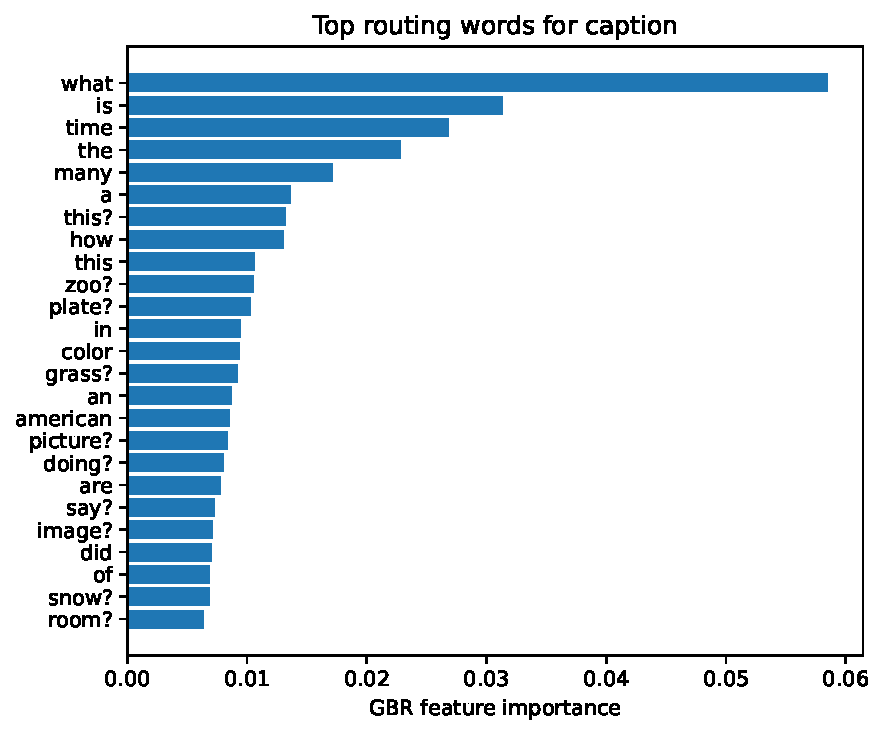
\includegraphics[width=0.49\linewidth]{plots/routing_words_caption.pdf}}
\hfill
\subfloat[Full-resolution need]{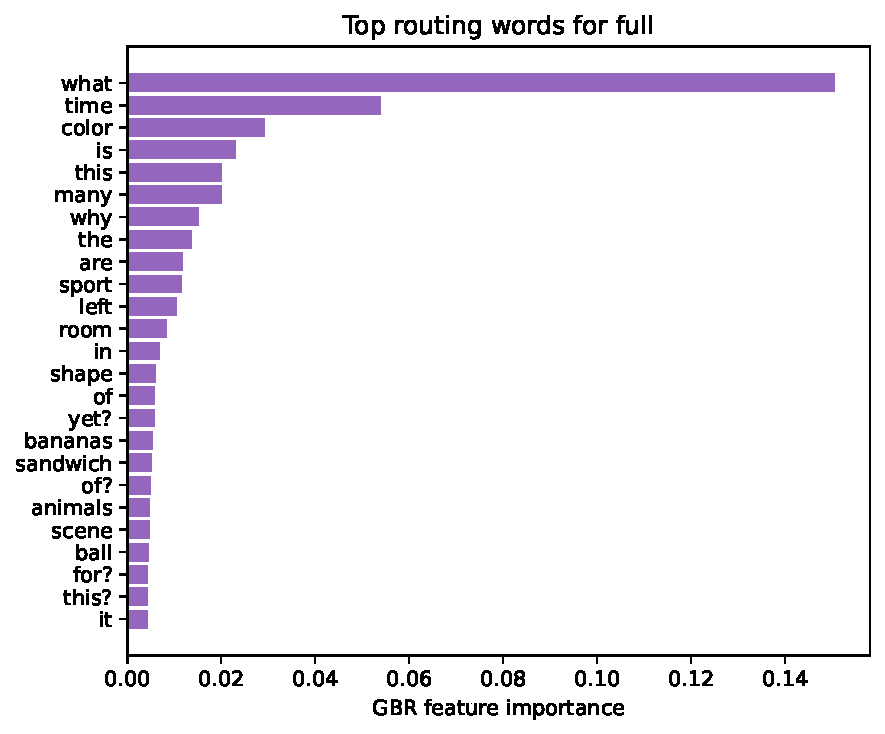
\includegraphics[width=0.49\linewidth]{plots/routing_words_full.pdf}}
\caption{\textbf{Top TF-IDF feature importances} learned by the GBR routing model (VQA-v2, Pixtral-12B). Words predictive of caption-level sufficiency (left) skew toward semantically coarse queries (\emph{is}, \emph{there}); those predicting full-resolution need (right) include visually specific terms (\emph{color}, \emph{many}, \emph{sport}).}
\label{fig:routing_words}
\end{figure}

\subsection*{Iso-Accuracy Contours: Fidelity vs.\ Model Scale}

\begin{figure}[htb]
\centering
\subfloat[VQA-v2]{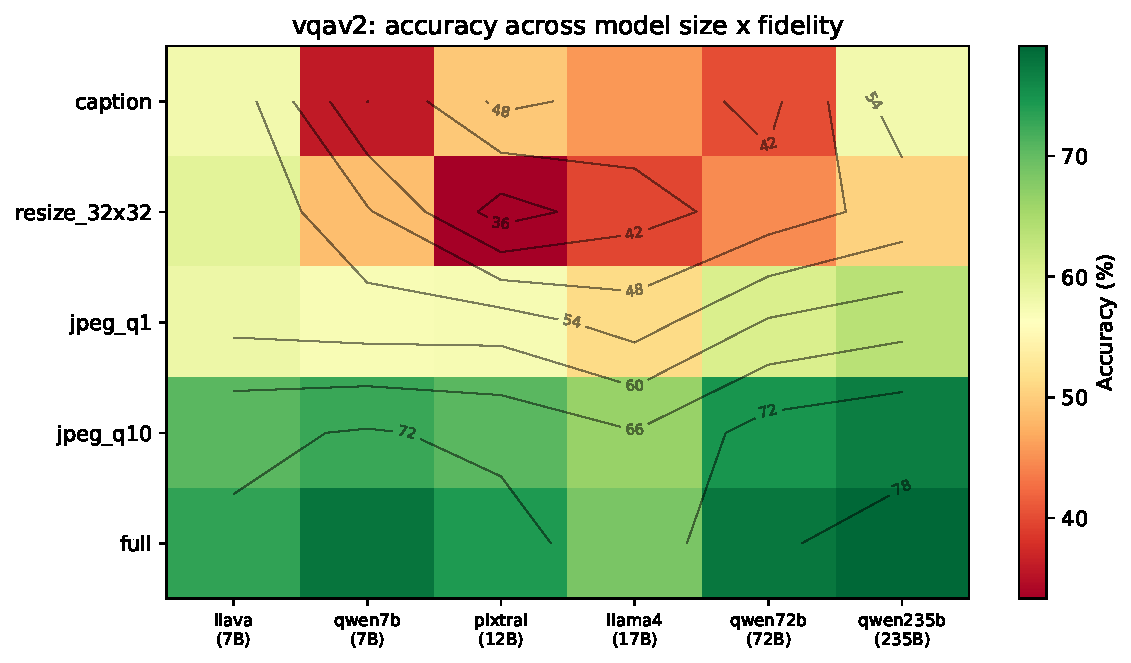
\includegraphics[width=0.49\linewidth]{plots/iso_accuracy_contour_vqav2.pdf}}
\hfill
\subfloat[GQA]{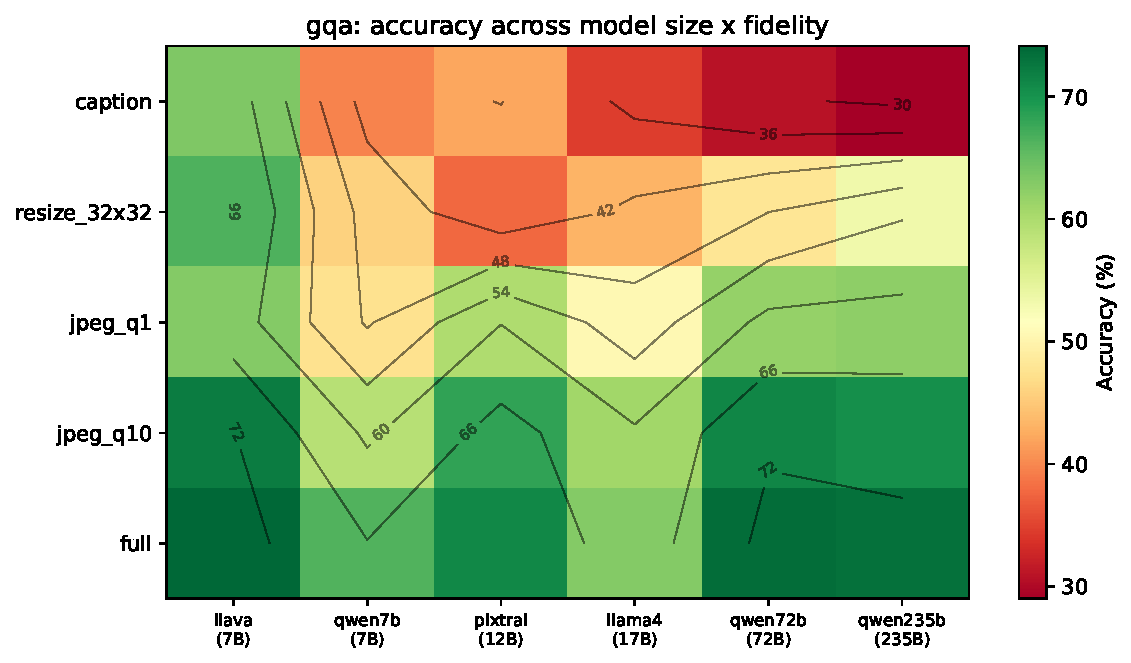
\includegraphics[width=0.49\linewidth]{plots/iso_accuracy_contour_gqa.pdf}}
\caption{\textbf{Iso-accuracy contours} showing VQA accuracy as a joint function of model scale and input fidelity. Contour lines connect (model, fidelity) pairs achieving equal accuracy. Fidelity improvements provide gains comparable to large model-scale jumps: a 7B model at JPEG Q10 often matches a 235B model at caption fidelity (Observation~3). The contours quantify why fidelity and model capacity are complementary, not substitutable, optimization dimensions.}
\label{fig:iso_accuracy_contour}
\end{figure}

\subsection*{Reliability Diagrams: Calibration Quality Across Settings}

\begin{figure}[htb]
\centering
\subfloat[VQA-v2 / Pixtral-12B]{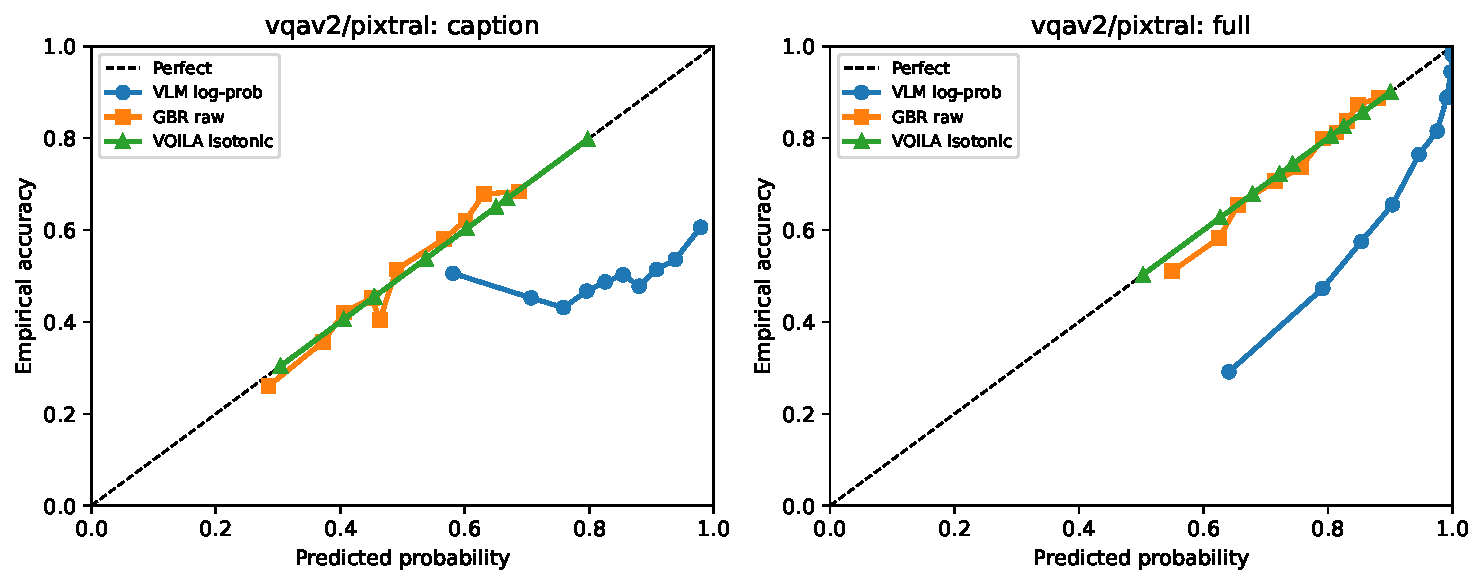
\includegraphics[width=0.49\linewidth]{plots/reliability_vqav2_pixtral.pdf}}
\hfill
\subfloat[GQA / Qwen2.5-VL-7B]{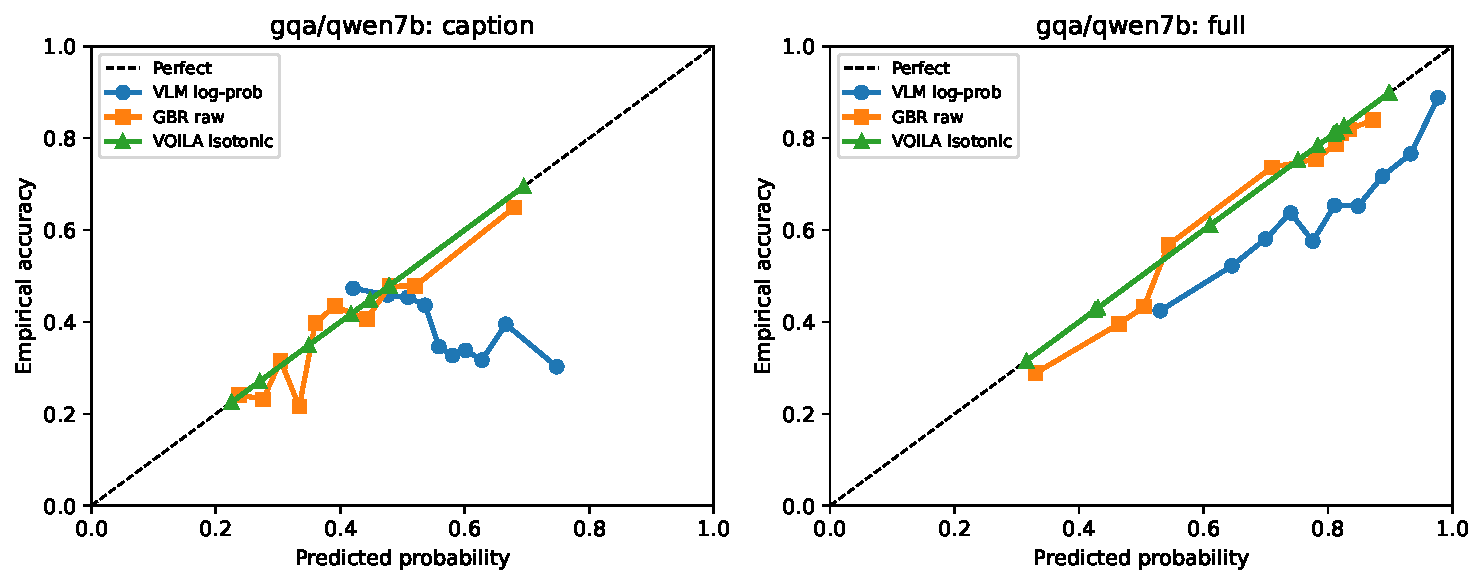
\includegraphics[width=0.49\linewidth]{plots/reliability_gqa_qwen7b.pdf}}
\caption{\textbf{Reliability diagrams} comparing VLM log-probability confidence, raw GBR scores, and isotonic-calibrated VOILA probabilities against the perfect-calibration diagonal (dashed). Isotonic calibration closely tracks the diagonal across both model--dataset pairs; ECE reduces from 0.025 to 0.012 (VQA-v2/Pixtral) and from 0.042 to 0.020 (GQA/Qwen7B).}
\label{fig:reliability}
\end{figure}

\subsection*{Score Separation: Calibrated vs.\ Uncalibrated Predictions}

\begin{figure}[htb]
\centering
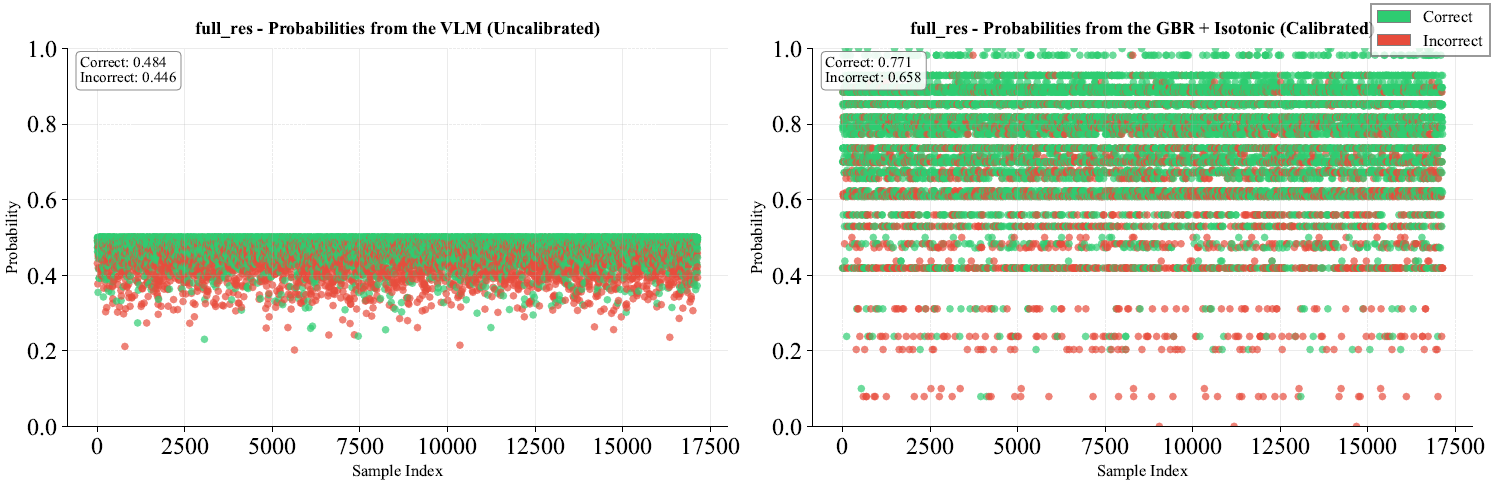
\includegraphics[width=\linewidth]{plots/calibration_uncalibration_img.png}
\caption{\textbf{Score separation before and after isotonic calibration} (VQA-v2, Pixtral-12B, caption fidelity). Each point is a query, colored by outcome (correct/incorrect). Raw GBR scores overlap substantially between correct and incorrect predictions, making threshold-based escalation unreliable. After isotonic calibration, correct predictions cluster toward higher probabilities and incorrect predictions toward lower values, enabling reliable expected-value computations in the VOI criterion.}
\label{fig:calibration_scatter}
\end{figure}

\subsection*{ROC Curves for Escalation Decisions}

\begin{figure}[htb]
\centering
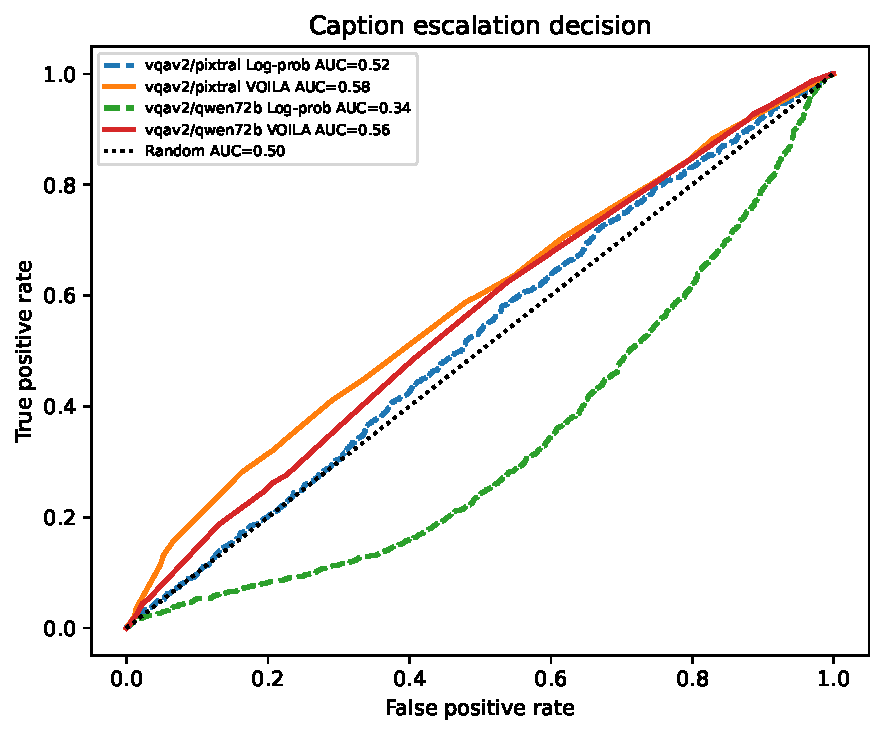
\includegraphics[width=0.92\linewidth]{plots/roc_escalation_decision.pdf}
\caption{\textbf{ROC curves for caption-to-full escalation decisions} (VQA-v2). A positive example is a query where caption fidelity fails but full resolution succeeds. \textsc{VOILA}'s question-conditioned score (AUC\,=\,0.581) outperforms log-probability thresholding (AUC\,=\,0.522) for Pixtral-12B. For Qwen2-VL-72B, the log-probability AUC falls to 0.338---below random (dashed)---confirming that VLM confidence is actively anti-correlated with the need to escalate for this model.}
\label{fig:roc_escalation}
\end{figure}

\begin{table*}[p]
\centering
\tiny
\caption{
\textbf{Extended Calibration Ablation Across All Models (VQA-v2 and GQA).}
Each entry reports \textbf{Acc (\%) / Cost}.
We evaluate three calibration methods (None, Isotonic, Temperature Scaling) and two alternative decision rules (Accuracy-only, Fixed-threshold) across six VLMs.
\emph{Iso} (isotonic, \textsc{VOILA} default) is bolded; it consistently achieves the strongest cost--accuracy Pareto position.
Fixed-resolution cost is 100; all other costs are normalized relative to this.
}
\label{tab:extended_ablation_all}\label{tab:ablation_calibration}
\resizebox{\linewidth}{!}{
\begin{tabular}{llccccc}
\toprule
\multirow{2}{*}{\textbf{Model}} & \multirow{2}{*}{\textbf{Method}}
& \multicolumn{3}{c}{\textbf{Calibration Variants (VOI Routing)}}
& \multicolumn{2}{c}{\textbf{Alternative Decision Rules (Isotonic)}} \\
\cmidrule(lr){3-5}\cmidrule(lr){6-7}
& & \textbf{None} & \textbf{Isotonic} & \textbf{Temp. Scaling}
& \textbf{Acc-only} & \textbf{Fixed-Thr.} \\
\midrule
\multicolumn{7}{c}{\textit{\textbf{VQA-v2}}} \\
\midrule
Pixtral-12B
& Acc / Cost
& 67.4 / 47.6
& \textbf{64.1 / 38.7}
& 66.5 / 45.3
& 74.2 / 100.0
& 59.7 / 32.2 \\

Llama-4-Maverick
& Acc / Cost
& 60.5 / 38.5
& \textbf{59.7 / 37.1}
& 60.7 / 39.6
& 68.4 / 100.0
& 56.6 / 33.9 \\

Qwen2-VL-72B
& Acc / Cost
& 67.3 / 43.2
& \textbf{64.4 / 37.3}
& 65.8 / 40.7
& 77.6 / 100.0
& 57.8 / 31.0 \\

LLaVA-1.5-7B
& Acc / Cost
& 67.9 / 34.5
& \textbf{66.5 / 26.2}
& 67.8 / 32.7
& 73.1 / 100.0
& 62.5 / 18.0 \\

Qwen2.5-VL-7B
& Acc / Cost
& 63.4 / 34.3
& \textbf{63.1 / 34.1}
& 64.3 / 36.7
& 77.8 / 100.0
& 61.4 / 33.5 \\

Qwen3-VL-235B
& Acc / Cost
& 71.1 / 33.6
& \textbf{71.5 / 37.4}
& 71.3 / 34.6
& 79.1 / 100.0
& 62.9 / 17.5 \\

\midrule
\multicolumn{7}{c}{\textit{\textbf{GQA}}} \\
\midrule
Pixtral-12B
& Acc / Cost
& 61.2 / 32.6
& \textbf{60.4 / 31.1}
& 61.1 / 31.4
& 71.1 / 100.0
& 59.1 / 34.5 \\

Llama-4-Maverick
& Acc / Cost
& 52.3 / 26.2
& \textbf{53.4 / 29.5}
& 53.5 / 29.4
& 62.9 / 100.0
& 53.7 / 40.0 \\

Qwen2-VL-72B
& Acc / Cost
& 60.1 / 30.8
& \textbf{60.0 / 28.9}
& 60.3 / 30.5
& 73.5 / 100.0
& 58.3 / 30.7 \\

LLaVA-1.5-7B
& Acc / Cost
& 70.0 / 29.3
& \textbf{69.5 / 25.9}
& 70.0 / 30.4
& 74.1 / 100.0
& 65.0 / 12.1 \\

Qwen2.5-VL-7B
& Acc / Cost
& 57.2 / 33.5
& \textbf{55.0 / 27.8}
& 56.7 / 32.8
& 66.2 / 100.0
& 53.2 / 47.0 \\

Qwen3-VL-235B
& Acc / Cost
& 59.9 / 26.8
& \textbf{59.0 / 24.3}
& 59.4 / 24.1
& 73.2 / 100.0
& 59.9 / 32.3 \\

\bottomrule
\end{tabular}
}
\end{table*}

\begin{table}[p]
\centering
\small
\caption{
\textbf{Predictor Robustness Under Fixed Isotonic Calibration (Pixtral-12B).}
Each entry reports \textbf{Acc (\%) / Cost}.
Performance is broadly similar across predictor architectures once calibration is applied, demonstrating that \textsc{VOILA}'s gains stem from calibration and VOI routing rather than predictor choice.
GBR (\textsc{VOILA} default) is bolded.
}
\label{tab:predictor_robustness_extended}
\label{tab:predictor_robustness_pixtral}
\setlength{\tabcolsep}{5pt}
\begin{tabular}{lcccc}
\toprule
\textbf{Dataset} & \textbf{GBR} & \textbf{LogReg} & \textbf{Ridge} & \textbf{MLP} \\
\midrule
VQA-v2 & \textbf{64.1 / 38.8} & 65.0 / 43.4 & 63.9 / 40.0 & 63.4 / 38.4 \\
GQA    & \textbf{60.5 / 31.1} & 60.2 / 30.6 & 59.6 / 29.9 & 60.3 / 31.6 \\
\bottomrule
\end{tabular}
\end{table}


This section provides a comprehensive analysis of \textsc{VOILA}'s design choices, expanding on the ablation results summarized in the main paper.
We evaluate calibration methods and decision rules across six VLMs and two datasets (VQA-v2 and GQA), and assess predictor robustness for Pixtral-12B.

\subsection{Experimental Design}
\label{sec:ablation_design}

We evaluate three dimensions of design choices:

\textbf{Calibration methods.} We compare three approaches to converting raw predictor scores into probabilities suitable for utility estimation:
\begin{itemize}[leftmargin=*,nosep]
\item \textit{None}: Raw GBR scores used directly without post-hoc calibration.
\item \textit{Isotonic}: Isotonic regression applied to raw scores (\textsc{VOILA} default), enforcing monotonicity while remaining non-parametric.
\item \textit{Temperature scaling}: A standard post-hoc calibration method from classification literature~\cite{guo2017calibrationmodernneuralnetworks}, included as a negative control.
\end{itemize}

\textbf{Decision rules.} Given calibrated predictors, we compare VOI routing against two alternative strategies:
\begin{itemize}[leftmargin=*,nosep]
\item \textit{Accuracy-only}: Always select the fidelity with highest predicted correctness probability, ignoring acquisition cost. Represents an unconstrained accuracy-maximizing baseline.
\item \textit{Fixed-threshold}: Escalate to higher fidelity only when predicted probability falls below a fixed cutoff tuned on held-out VQA-v2 data.
\end{itemize}

\textbf{Predictor architectures.} We evaluate four question-conditioned regressors under fixed isotonic calibration for Pixtral-12B: Gradient Boosting (GBR, \textsc{VOILA} default), Logistic Regression, Ridge Regression, and MLP. All use identical question features.

\subsection{Comprehensive Results}
\label{sec:ablation_results}

Table~\ref{tab:extended_ablation_all} reports accuracy and cost for each ablation across 12 model--dataset combinations.

\paragraph{Isotonic calibration consistently improves the cost--accuracy tradeoff.}
Comparing columns 1--2 in Table~\ref{tab:extended_ablation_all}, isotonic calibration achieves lower cost than uncalibrated routing while maintaining comparable accuracy.
For example, on VQA-v2 with LLaVA-1.5-7B, uncalibrated routing achieves 67.9\% at cost 34.5, whereas isotonic calibration achieves 66.5\% at cost 26.2 --- a 24\% cost reduction with only 1.4 point accuracy sacrifice.
On GQA with Pixtral-12B, isotonic routing achieves 60.4\% at cost 31.1 versus uncalibrated 61.2\% at cost 32.6.
The advantage is most pronounced when predictions are overconfident at low fidelity: calibration corrects this, reducing unnecessary escalation.

\paragraph{Calibration improves routing efficiency, not task accuracy.}
Calibration does not alter which visual information is processed or how the VLM reasons; it improves \emph{routing decisions} by producing reliable probability estimates.
Isotonic regression's monotonicity constraint ensures that utility differences $\hat{p}_{k+1}(q) - \hat{p}_k(q)$ reliably indicate when escalation is beneficial, a property that general-purpose calibrators like temperature scaling do not enforce.

\paragraph{Temperature scaling is not appropriate for cost-sensitive sequential decisions.}
Temperature scaling (column 3) often increases cost relative to isotonic calibration without accuracy gains.
On VQA-v2 with Pixtral, temperature scaling achieves 66.5\% at cost 45.3 versus isotonic's 64.1\% at cost 38.7 --- 17\% higher cost.
The instability reflects temperature scaling's optimization of global calibration metrics (log-loss) that do not align with cross-fidelity utility ordering.

\subsection{Why VOI Routing Dominates Heuristic Baselines}
\label{sec:voi_dominance}

\paragraph{Accuracy-only selection: the cost of ignoring resources.}
The accuracy-only baseline (column 4) always retrieves at cost 100 (full resolution by construction), representing 60--170\% cost inflation over \textsc{VOILA} depending on the setting.
The accuracy gain is marginal: for Qwen3-VL-235B on VQA-v2, accuracy-only achieves 79.1\% versus \textsc{VOILA}'s 71.5\% --- an 7.6 point gap at 170\% cost inflation.
For LLaVA-1.5-7B on GQA, the gap is only 4.6 points (74.1\% vs.\ 69.5\%) at 286\% cost inflation, confirming that most queries do not require maximum-fidelity inputs.

\paragraph{Fixed-threshold heuristics: brittleness without adaptivity.}
The fixed-threshold baseline (column 5) shows inconsistent behavior across settings.
On GQA with LLaVA-1.5-7B, it achieves 65.0\% at cost 12.1 --- lower cost than \textsc{VOILA}'s 69.5\% at 25.9 but with 4.5 point accuracy loss, suggesting over-aggressive escalation avoidance.
On GQA with Qwen2.5-VL-7B, it achieves 53.2\% at cost 47.0 --- higher cost than \textsc{VOILA}'s 55.0\% at 27.8 with 1.8 point accuracy loss, showing under-escalation on visually demanding queries.
This dataset- and model-dependent behavior requires per-setting retuning, whereas \textsc{VOILA}'s VOI criterion adapts automatically.

\subsection{Robustness to Predictor Architecture}
\label{sec:predictor_robustness}

Table~\ref{tab:predictor_robustness_extended} evaluates four predictors for Pixtral-12B under isotonic calibration.
On VQA-v2, GBR achieves 64.1\% at cost 38.8 while LogReg achieves 65.0\% at cost 43.4, Ridge achieves 63.9\% at cost 40.0, and MLP achieves 63.4\% at cost 38.4.
The accuracy spread (1.6 points) and cost spread (5.0 units) are small relative to the gains from calibration itself.
On GQA, the spread is even smaller: 60.2--60.5\% accuracy and 29.9--31.6 cost.
This robustness validates that \textsc{VOILA}'s performance is driven by calibration quality and VOI routing, not predictor expressivity.
System designers can choose predictors based on deployment constraints (memory, latency, retraining frequency) without sacrificing core benefits.

\subsection{Key Takeaways and Design Implications}
\label{sec:takeaways}

Our extended ablation studies establish four findings:

\textbf{(1) Calibration is essential, but method choice matters.}
Isotonic regression is well-suited for cost-sensitive sequential decisions because it enforces cross-fidelity monotonicity.
General-purpose methods like temperature scaling optimize global metrics that do not align with routing quality.

\textbf{(2) VOI routing dominates heuristics across the cost--accuracy frontier.}
Accuracy-only selection over-retrieves; fixed thresholds under- or over-retrieve unpredictably.
\textsc{VOILA} achieves Pareto optimality by reasoning about marginal utility via calibrated probabilities, without per-dataset retuning.

\textbf{(3) \textsc{VOILA} is robust to implementation choices.}
The same pipeline yields consistent gains across six VLMs (7B--235B), two datasets, and four predictor architectures.

\textbf{(4) The framework is complementary to model routing.}
\textsc{VOILA} optimizes \emph{what to retrieve before model execution}; model routing optimizes \emph{which model to apply after retrieval}.
These axes are orthogonal and can be combined for end-to-end efficiency in multimodal systems.

\subsection*{Log-prob Cascade Degeneracy}

\begin{table}[htb]
\centering
\small
\setlength{\tabcolsep}{3pt}
\caption{\textbf{Log-prob Cascade degeneracy} (representative cases). Near-zero escalation rates indicate the cascade never leaves caption fidelity (underconfidence failure); near-100\% rates indicate it always escalates to full resolution (overconfidence failure). Averaged across all 24 model--dataset pairs, the cascade escalates in 50\% of queries at cost 39.7, vs.\ \textsc{VOILA}'s cost of 27.3.}
\label{tab:cascade_degeneracy}
\begin{tabular}{llcc}
\toprule
\textbf{Model} & \textbf{Dataset} & \textbf{Escalation rate} & \textbf{Avg.\ cost} \\
\midrule
\multicolumn{4}{l}{\textit{Degenerate: never escalates}} \\
Qwen2-VL-72B  & TextVQA & 0.00\% & 7.6 \\
Qwen2-VL-72B  & GQA     & 0.03\% & 7.6 \\
Qwen2-VL-72B  & VQA-v2  & 0.18\% & 7.7 \\
LLaMA-4-Mav.  & GQA     & 0.28\% & 7.8 \\
\midrule
\multicolumn{4}{l}{\textit{Degenerate: always escalates}} \\
Qwen3-VL-235B & GQA     & 99.96\% & 83.8 \\
Qwen2.5-VL-7B & GQA     & 99.78\% & 74.8 \\
\midrule
\textit{Overall avg.} & all & 50.0\% & 39.7 \\
\bottomrule
\end{tabular}
\end{table}


% -----------------------------------------------------------------------
% REWRITTEN related work — added VQA foundations, query difficulty,
% multimodal RAG, and FrugalGPT cascade distinction; all existing
% paragraphs expanded
% -----------------------------------------------------------------------

\section{Extended Related Work}\label{sec:related_ext}

\noindent\textbf{Visual Question Answering.}
VQA~\cite{antol2015vqa} introduced the task of answering free-form natural language questions about images.
VQA-v2~\cite{goyal2017vqav2} reduced language-prior biases via complementary image pairs; GQA~\cite{hudson2019gqa} introduced compositional reasoning over scene graphs; TextVQA~\cite{singh2019textvqa} highlighted OCR-dependent visual understanding.
Analysis of VQA performance has consistently found that question type is strongly predictive of model accuracy and failure modes: counting and text-recognition questions are universally harder, while yes/no questions are systematically easier~\cite{kafle2017analysis, agrawal2018dont}.

\noindent\textbf{Pre-Retrieval Query Difficulty Estimation.}
Estimating query difficulty before retrieval---from query features alone---is a longstanding problem in information retrieval~\cite{zhao2008predicting, hauff2008improved, mothe2005linguistic}.
These methods use lexical, syntactic, and statistical properties of the query to predict retrieval quality without executing the retrieval step, enabling cost-aware allocation of retrieval resources.
VOILA adapts this paradigm to multimodal perception: we estimate, from question-linguistic features alone, the probability that a VLM succeeds at each visual fidelity---without executing the VLM or accessing any image.
This makes VOILA a direct generalization of pre-retrieval query difficulty estimation to the cross-modal, cost-sensitive fidelity selection setting.

\noindent\textbf{FrugalGPT-Style Cascades and Confidence-Based Routing.}
FrugalGPT~\cite{chen2023frugalgpt} reduces LLM inference cost by routing queries through a cascade of models in ascending cost order, using the cheapest model that produces a sufficiently confident answer~\cite{shnitzer2023large, wang2024routellm}.
Adapted to fidelity selection, this yields a natural \emph{sequential cascade baseline}: run the VLM at the lowest fidelity; if output log-probability falls below a threshold, escalate to the next fidelity; repeat until confident.
VOILA differs from this paradigm in two fundamental ways.
First, the cascade is \emph{post-retrieval}---it incurs retrieval and VLM inference costs at every intermediate fidelity before reaching the final answer, meaning it cannot avoid the costs it aims to minimize.
Second, cascades rely on the VLM's own confidence as the escalation signal, which Observation 2 shows is unreliable when visual context is insufficient: the VLM produces confident-but-wrong answers at low fidelity, so the cascade does not escalate when it should.
VOILA avoids both problems by selecting the target fidelity \emph{before any retrieval} using question-conditioned prediction, eliminating intermediate costs and bypassing post-hoc confidence signals entirely.
We compare directly against a log-prob cascade baseline in \S\ref{sec:results}.

\noindent\textbf{Adaptive Inference and Model Routing.}
Beyond FrugalGPT, a broad line of work studies adaptive computation for NLP: early-exit transformers~\cite{zhou2020bert, elbayad2020depth} skip layers for ``easy'' inputs; CALM~\cite{schuster2022confident} exits generation early when token confidence is sufficient; RouteLLM~\cite{wang2024routellm} and hybrid routing~\cite{ding2024hybrid} dispatch queries across model tiers based on predicted difficulty.
All of these methods \emph{assume the input context is fully available} and optimize the computation applied to it.
VOILA is orthogonal: it optimizes \emph{what input context to acquire} before any computation begins, and can be composed with model routing to jointly optimize retrieval and inference costs.

\noindent\textbf{Adaptive Visual Resolution and Concurrent Work.}
A concurrent line of work addresses adaptive resolution selection for visual inputs.
CARES~\cite{kimhi2025cares} selects the minimal sufficient input resolution for a given image-query pair before forwarding to the target VLM, using a compact VLM to extract query-conditioned features from the image.
Prompt-guided prefiltering~\cite{azizian2026promptguided} identifies spatially task-relevant regions within an already-retrieved image before compression.
Both approaches reduce VLM compute or transmission cost, but both still require \emph{image access} to make the resolution or region decision.
VOILA is distinguished by its strictly pre-retrieval setting: in tiered-storage RAG systems, the image has not been fetched when the routing decision must be made.
VOILA therefore operates exclusively from question text---a strictly harder setting that eliminates retrieval cost at the source rather than reducing processing cost afterward.
Post-retrieval token compression~\cite{weng2024learning} and lightweight cross-modal fusion~\cite{farazi2021accuracy} reduce the cost of \emph{processing} a retrieved image; \textsc{VOILA} is complementary, deciding which representation to acquire in the first place.
% TODO before submission: verify kimhi2025cares (arxiv:2510.19496) and azizian2026promptguided (arxiv:2604.00314) are in example_paper.bib

\noindent\textbf{Multimodal Retrieval-Augmented Generation.}
Retrieval-augmented generation (RAG)~\cite{lewis2020rag} extends language models with retrieved context; multimodal extensions retrieve images, video frames, or memory traces~\cite{yasunaga2023retrievalaugmented, chen2022murag}.
In agentic memory settings~\cite{park2023generative, wang2024locomo}, agents must decide which stored memories to retrieve given a query.
All existing multimodal RAG frameworks treat retrieval as binary (retrieve or not) and assume a fixed representation quality for whatever is retrieved.
\textsc{VOILA} introduces a finer-grained retrieval decision: \emph{at what fidelity to retrieve}.

\noindent\textbf{Value-of-Information and Cost-Sensitive Acquisition.}
The value-of-information (VOI) framework~\cite{bilgic2011value} formalizes the expected utility of acquiring additional evidence given current beliefs.
Budgeted feature acquisition~\cite{karkkainen2019cost} and active acquisition in multimodal settings~\cite{kossen2022active} apply VOI to tabular and sequential data.
VOILA is the first to apply VOI to pre-retrieval fidelity selection in visual question answering, where the ``features'' are not tabular attributes but image representations at different compression levels, and the action space is structured by a physical retrieval cost function over storage tiers.

% -----------------------------------------------------------------------
% OLD RELATED WORK (kept for reference)
% -----------------------------------------------------------------------
\begin{comment}
\noindent\textbf{Adaptive Inference and Model Routing (old).}
Prior work studies adaptive computation by routing queries across models or dynamically allocating compute, including early-exit and adaptive depth mechanisms \cite{zhou2020bert, schuster2022confident} and cost-aware LLM routing \cite{chen2023frugalgpt, shnitzer2023large, ding2024hybrid, wang2024routellm}.
These methods optimize \emph{how} inference is performed given fixed inputs, whereas VOILA focuses on \emph{what information} to retrieve before inference.

\noindent\textbf{Systems Context for Multimodal Retrieval (old).}
Multimodal systems commonly store visual data across heterogeneous tiers, motivating retrieval-aware optimization.
Related work examines tiered storage and retrieval costs in cloud and mobile systems \cite{hort2021survey, zhang2024autonomous}, as well as agentic memory and long-horizon multimodal reasoning \cite{park2023generative, wang2024locomo}.
VOILA explicitly exploits this structure by selecting the minimum sufficient fidelity before accessing higher-cost tiers.
\end{comment}


\end{document}
